%  LaTeX support: latex@mdpi.com 
%  For support, please attach all files needed for compiling as well as the log file, and specify your operating system, LaTeX version, and LaTeX editor.

%=================================================================
\documentclass[sensors,article,accept,pdftex,moreauthors]{Definitions/mdpi} 
%\documentclass[preprints,article,submit,pdftex,moreauthors]{Definitions/mdpi} 
% For posting an early version of this manuscript as a preprint, you may use "preprints" as the journal. Changing "submit" to "accept" before posting will remove line numbers.

%\usepackage[utf8]{inputenc}
%%%%%%%%%%%%%%%
% \usepackage[disable]{todonotes}
%\usepackage{todonotes}


\usepackage[per-mode=symbol]{siunitx}
\sisetup{round-mode=places,round-precision=2,round-pad=false} % figures: significative, places: decimal
\sisetup{inter-unit-product = \ensuremath { { } {\cdot} { } }} % m.s.K.s-1
\DeclareSIUnit{\rad}{rad}
\DeclareSIUnit{\deg}{deg}
\usepackage[english]{babel}
\usepackage{circuitikz}
\usepackage[labelformat=simple]{subcaption}
\renewcommand\thesubfigure{\alph{subfigure}}
\DeclareCaptionLabelFormat{subcaptionlabel}{\normalfont(\textbf{#2}\normalfont)}
\captionsetup[subfigure]{labelformat=subcaptionlabel}

\usepackage{lineno}
\usepackage{wasysym}
\usepackage{physics}
\usepackage{booktabs}
\usepackage{multicol}
\usepackage{multirow}
% \linenumbers % Turn off line numbering for Optica Open preprint submissions.
%% Add by roney
% \usepackage[nameinlink]{cleveref} % references
% \usepackage[acronym,symbols,toc, automake=true,translate=babel,nomain, nonumberlistz]{glossaries-extra}

\usepackage[acronym,%
  symbols,%
  toc=false,
  automake=false,
  translate=babel,
  nonumberlist,
  % hyperoutside=true,
  % numberedsection=autolabel,
  % sanitize={none},
  nomain]{glossaries}
\usepackage{glossary-mcols}
\glsnoexpandfields
% \makeglossaries

% adiciona o campo de unidades
%\usepackage{glossary-mcols}%multi-column styles

\newglossarystyle{supergroup}{%
  % \setglossarystyle{super3col}%
  \setglossarystyle{long3colheader}%
  \renewcommand*{\glossaryheader}{%
    \bfseries Símbolo  & \bfseries Descrição & \bfseries Unidade \\\hline}%
  \setlength{\glsdescwidth}{0.7\textwidth}%
  \renewcommand*{\glsgroupskip}{}%
  \renewcommand{\glossentry}[2]{%
    \tabularnewline
    \multicolumn{2}{c}{%
      \bfseries\glsentryitem{##1}\glstarget{##1}{\glossentryname{##1}}%
    }%
    \tabularnewline
    & \glossentrydesc{##1}%\glspostdescription
    \tabularnewline
  }%
  \renewcommand{\subglossentry}[3]{%
    \glssubentryitem{##2}%
    \glstarget{##2}{\glossentryname{##2}}
    &
    \glossentrydesc{##2}\glspostdescription
    &
    \glsentryunit{##2}%{##3}%\space\space
    \tabularnewline
  }%
}
\glsaddkey{unit}{\glsentrytext{\glslabel}}{\glsentryunit}{\GLsentryunit}{\glsunit}{\Glsunit}{\GLSunit}

%\newglossary{estimador}{est}{estl}{Símbolos do estimador}
\newglossaryentry{gps}
{type=\acronymtype,
  name={GPS},
  user1 = {\foreignlanguage{english}{Global Position System}},
  description={\foreignlanguage{english}{Global Position System}},
  first = {Global Position System (GPS)}
}

\newglossaryentry{glonass}
{type=\acronymtype,
  name={GLONASS},
  user1 = {\foreignlanguage{english}{Global Navigational Satellite System}},
  description={\foreignlanguage{english}{Global Navigational Satellite System}},
  %first = {Sistema Global de Navegação por Satélites (GLONASS, \foreignlanguage{english}{Global Navigational Satellite System})}
  first = {GLONASS (\foreignlanguage{english}{Global Navigational Satellite System})}
}

\newglossaryentry{cfbg}
{type=\acronymtype,
  name={CFBG},
  user1 = {chirped fiber Bragg gratings},
  description={chirped fiber Bragg gratings},
  first = {\glsentryuseri{cfbg} (\glsentryname{cfbg})}
}
\newglossaryentry{galileo}
{type=\acronymtype,
  name={Galileo},
  user1 = {\foreignlanguage{english}{European Global Navigation Satellite System}},
  description={\foreignlanguage{english}{European Global Navigation Satellite System}},
  %first = {Sistema Global de Navegação por Satélites Europeu (Galileo, \foreignlanguage{english}{European Global Navigation Satellite System})}
  first = {Galileo (\foreignlanguage{english}{European Global Navigation Satellite System})}
}

\newglossaryentry{beidou}
{type=\acronymtype,
  name={BeiDou},
  user1 = {BeiDou Navigation Satellite System},
  description={\glsentryuseri{beidou}},
  first = {\glsentryname{beidou} (BDS, \glsentryuseri{beidou})}
}

\newglossaryentry{ecef}
{type=\acronymtype,
  name={ECEF},
  user1 = {\foreignlanguage{english}{Earth centered Earth fixed}},
  description={\glsentryuseri{ecef}},
  first = {centralizado e fixo na Terra (ECEF, \glsentryuseri{ecef})}
}
\newglossaryentry{mcd}
{type=\acronymtype,
  user1={matriz de cossenos diretores},
  name={MCD},
  description={\titlecap{\glsentryuseri{mcd}}},
  first = {\glsentryuseri{mcd} (\glsentryname{mcd})}
}

\newglossaryentry{sdre}
{type=\acronymtype,
  name={SDRE},
  symbol={SDRE},
  user1 = {state dependent Riccati equation},
  description={\foreignlanguage{english}{\glsentryuseri{sdre}}},
  first = {equação de Riccati dependente dos estados (SDRE, \foreignlanguage{english}{\glsentryuseri{sdre}})}
}

\newglossaryentry{lqr}
{type=\acronymtype,
  name={LQR},
  description={\foreignlanguage{english}{\glsentryuseri{lqr}}},
  user1 = {linear quadratic regulator},
  first = {regulador linear quadrático (LQR, \foreignlanguage{english}{\glsentryuseri{lqr}})}
}

\newglossaryentry{lqt}
{type=\acronymtype,
  name={LQT},
  description={\foreignlanguage{english}{\glsentryuseri{lqt}}},
  user1 = {linear quadratic tracking},
  first = {rastreador linear quadrático (\glsentryname{lqt}, \foreignlanguage{english}{\glsentryuseri{lqt}})}
}

\newglossaryentry{pid}
{type=\acronymtype,
  name={PID},
  description={proporcional, integral e derivativo},
  first = {proporcional, integral e derivativo (PID)}
}

\newglossaryentry{pd}
{type=\acronymtype,
  name={PD},
  description={proporcional derivativo},
  first = {proporcional derivativo (PD)}
}

\newglossaryentry{vant}
{type=\acronymtype,
  name={VANT},
  plural={VANTs},
  description={veículo aéreo não tripulado},
  first = {veículo aéreo não tripulado (VANT ou UAV, do Inglês, \foreignlanguage{english}{Unmanned Aerial Vehicle})},
  firstplural = {veículos aéreos não tripulados (VANTs ou UAVs, do Inglês, \foreignlanguage{english}{Unmanned Aerial Vehicles})}
}
\newglossaryentry{fk}
{type=\acronymtype,
  name={KF},
  user1 = {\foreignlanguage{english}{Kalman filter}},
  description=\glsentryuseri{fk},
  first = {filtro de Kalman (\glsentryname{fk}, \glsentrydesc{fk})}
}


\newglossaryentry{ekf}
{type=\acronymtype,
  name={EKF},
  user1 = {\foreignlanguage{english}{extended Kalman filter}},
  description={\glsentryuseri{ekf}},
  first = {filtro de Kalman estendido (EKF, \glsentrydesc{ekf})}
}

\newglossaryentry{mekf}
{type=\acronymtype,
  name={MEKF},
  user1 = {multiplicative extended Kalman filter},
  description=\glsentryuseri{mekf},
  first = {filtro de Kalman estendido (MEKF, \glsentryuseri{mekf})}
}

\newglossaryentry{erkf}
{type=\acronymtype,
  name={ErKF},
  user1 = \foreignlanguage{english}{error state Kalman filter},
  description={\glsentryuseri{erkf}},
  first = {filtro de Kalman estendido dos erros de estados (\glsentryname{erkf}, \glsentryuseri{erkf})}
}

\newglossaryentry{imu}
{type=\acronymtype,
  name={IMU},
  user1 = \foreignlanguage{english}{inertial measurement unit},
  description={\glsentryuseri{imu}},
  first = {\glsentryuseri{imu} (IMU)}
}

\newglossaryentry{vhsor}
{type=\acronymtype,
  name=VHSOR,
  description={Veículo híbrido submersível operado de forma Remota},
  first = {veículo híbrido submersível operado de forma remota (VHSOR)}
}

\newglossaryentry{ahrs}
{type=\acronymtype,
  name={AHRS},
  user1 ={\foreignlanguage{english}{attitude and heading reference system}},
  description={\glsentryuseri{ahrs}},
  first = {sistema de referência de atitude e direção (AHRS, \glsentryuseri{ahrs})}
}

\newglossaryentry{marg}
{type=\acronymtype,
  name={MARG},
  user1 = {\foreignlanguage{english}{magnetic, angular rate, and gravity}},
  description={\glsentryuseri{marg}},
  first = {campo magnético, velocidade angular e gravidade (MARG, \glsentryuseri{marg})}
}


\newglossaryentry{zoh}
{type=\acronymtype,
  name={ZOH},
  user1 = {zero order hold},
  description={\foreignlanguage{english}{\glsentryuseri{zoh}}},
  first = {retentor de ordem zero (ZOH, \foreignlanguage{english}{Zero Order Hold})}
}

\newglossaryentry{ned}
{type=\acronymtype,
  name={NED},
  user1={north-east-down},
  description={\foreignlanguage{english}{\glsentryuseri{ned}}},
  first = {norte-leste-baixo (NED, \foreignlanguage{english}{North-East-Down})}
}
\newglossaryentry{gnss}
{type=\acronymtype,
  user1 = {\foreignlanguage{english}{Global Navigation Satellite Systems}},
  description=\foreignlanguage{english}{Global Navigation Satellite System},
  name={GNSS},
  first = {\glsentrydesc{gnss} (GNSS)}
}
\newglossaryentry{mimo}
{type=\acronymtype,
  name={MIMO},
  description={multi-input multi-output},
  first = {múltiplas entradas e múltiplas saídas (MIMO, \foreignlanguage{english}{multi-input multi-output})}
}

\newglossaryentry{siso}
{type=\acronymtype,
  name={SISO},
  description={single-input single-output},
  first = {única-entrada e única-saída (\glsentryname{siso}, \glsentrydesc{siso})}
}

\newglossaryentry{ins}
{type=\acronymtype,
  user1={\foreignlanguage{english}{inertial navigation system}},
  name={INS},
  description={\glsentryuseri{ins}},
  first = {\glsentryuseri{ins} (INS)}
}

\newglossaryentry{mmq}
{type=\acronymtype,
  name={LSQ},
  user1 = {least squares method},
  description= {\glsentryuseri{mmq}},
  first = {\glsentryuseri{mmq} (\glsentryname{mmq})}
}

\newglossaryentry{triadAlgoritimo}
{type=\acronymtype,
  user1={\foreignlanguage{english}{tri-axial attitude determination}},
  name={TRIAD},
  description={\glsentryuseri{triadAlgoritimo}},
  first = {\glsentryname{triadAlgoritimo} (\glsentryuseri{triadAlgoritimo})}
}

\newglossaryentry{quest}
{type=\acronymtype,
  user1={\foreignlanguage{english}{quaternion estimator}},
  name={QUEST},
  description={\glsentryuseri{quest}},
  first = {\glsentryname{quest} (\glsentryuseri{quest})}
}

\newglossaryentry{foam}
{type=\acronymtype,
  user1={\foreignlanguage{english}{fast optimal matrix algorithm}},
  name={FOAM},
  description={\glsentryuseri{foam}},
  first = {\glsentryname{foam} (\glsentryuseri{foam})}
}
\newglossaryentry{svd}
{type=\acronymtype,
  user1={\foreignlanguage{english}{singular value decomposition}},
  name={SVD},
  description={\glsentryuseri{svd}},
  first = {\glsentryname{svd} (\glsentryuseri{svd})}
}


\newglossaryentry{rmse}
{type=\acronymtype,
  user1={\foreignlanguage{english}{root mean square error}},
  name={RMSE},
  description={\glsentryuseri{rmse}},
  first = {\glsentryuseri{rmse} (\glsentryname{rmse})}
}
\newglossaryentry{rms}
{type=\acronymtype,
  user1={\foreignlanguage{english}{root mean square}},
  name={RMS},
  description={\glsentryuseri{rms}},
  first = {\glsentryname{rms} (\glsentryuseri{rms})}
}
\newglossaryentry{flae}
{type=\acronymtype,
  user1={\foreignlanguage{english}{fast linear attitude estimator}},
  name={FLAE},
  description={\glsentryuseri{flae}},
  first = {\glsentryname{flae} (\glsentryuseri{flae})}
}

\newglossaryentry{fqa}
{type=\acronymtype,
  user1={\foreignlanguage{english}{factored quaternion algorithm}},
  name={FQA},
  description={\glsentryuseri{fqa}},
  first = {\glsentryname{fqa} (\glsentryuseri{fqa})}
}


\newglossaryentry{saam}
{type=\acronymtype,
  user1={\foreignlanguage{english}{super-fast attitude of accelerometer and magnetometer}},
  name={SAAM},
  description={\glsentryuseri{saam}},
  first = {\glsentryname{saam} (\glsentryuseri{saam})}
}

\newglossaryentry{nasa}
{type=\acronymtype,
  user1={{national aeronautics and space administration}},
  name={NASA},
  description={\glsentryuseri{nasa}},
  first = {\glsentryuseri{nasa} (\glsentryname{nasa})}
}

\newglossaryentry{cf}
{type=\acronymtype,
  user1={\foreignlanguage{english}{complementary filter}},
  name={CF},
  description={\glsentryuseri{cf}},
  first = {filtro complementar (\glsentryname{cf}, \glsentryuseri{cf})}
}
\newglossaryentry{dlpf}
{type=\acronymtype,
  user1=\foreignlanguage{english}{digital low-pass filter},
  name={DLPF},
  description={\glsentryuseri{dlpf}},
  first = {filtro passa-baixa digital (\glsentryname{dlpf}, \glsentryuseri{dlpf})}
}

\newglossaryentry{cad}
{type=\acronymtype,
  user1={\foreignlanguage{english}{computer aided design}},
  name={CAD},
  description={\glsentryuseri{cad}},
  first = {desenho assistido por computador (\glsentryname{cad}, \glsentryuseri{cad})}
}

\newglossaryentry{mems}
{type=\acronymtype,
  user1={\foreignlanguage{english}{micro-electro-mechanical systems}},
  name={MEMS},
  description={\glsentryuseri{mems}},
  first = {\glsentryuseri{mems} (\glsentryname{mems})},
  firstplural = {\glsentryuseri{mems} (\glsentryname{mems})}
}



\newglossaryentry{wb}
{type=\acronymtype,
  user1=\foreignlanguage{english}{band width},
  name={WB},
  description={\glsentryuseri{wb}},
  first = {largura de banda (\glsentryname{wb}, \glsentryuseri{wb})}
}

\newglossaryentry{pcnt}
{type=\acronymtype,
  user1=\foreignlanguage{english}{pulse counter},
  name={PCNT},
  description={\glsentryuseri{pcnt}},
  first = {\glsentryuseri{pcnt} (\glsentryname{pcnt})}
}


\newglossaryentry{sc}
{type=\acronymtype,
  name={SC},
  user1={sistema de coordenadas},
  user2={sistemas de coordenadas},
  description={\glsentryuseri{sc}},
  first = {sistema de coordenadas (\glsentryname{sc})},
  firstplural = {sistemas de coordenadas (\glsentryname{sc})}
}


\newglossaryentry{dcta}
{type=\acronymtype,
  name={DCTA},
  user1={Departamento de Ciência e Tecnologia Aeroespacial},
  description={\glsentryuseri{dcta} (originalmente Centro Técnico de Aeronáutica, CTA)},
  first = {\glsentryuseri{dcta} (\glsentryname{dcta})}
}

\newglossaryentry{ieav}
{type=\acronymtype,
  name={IEAv},
  user1={Instituto de Estudos Avançados},
  description={\glsentryuseri{ieav}},
  first = {\glsentryuseri{ieav} (\glsentryname{ieav})}
}

\newglossaryentry{iae}
{type=\acronymtype,
  name={IAE},
  user1={Instituto de Aeronáutica e Espaço},
  description={\glsentryuseri{iae}},
  first = {\glsentryuseri{iae} (\glsentryname{iae})}
}

\newglossaryentry{efo}
{type=\acronymtype,
  user1=Divisão de Fotônica,
  name={EFO},
  description={\glsentryuseri{efo}},
  first = { \glsentryuseri{efo} (\glsentryname{efo})}
}


\newglossaryentry{ifo}
{type=\acronymtype,
  user1=Unidade de Medição Inercial á Fibra Óptica,
  name={IFO},
  description={\glsentryuseri{ifo}},
  first = {\glsentryuseri{ifo} (\glsentryname{ifo})}
}

\newglossaryentry{cti}
{type=\acronymtype,
  name={CT\&I},
  user1={Ciência, Tecnologia e Inovação},
  description={\glsentryuseri{cti}},
  first = {\glsentryuseri{cti} (\glsentryname{cti})}
}

\newglossaryentry{comaer}
{type=\acronymtype,
  name={COMAER},
  user1={Comando da Aeronáutica},
  description={\glsentryuseri{comaer}},
  first = {\glsentryuseri{comaer} (\glsentryname{comaer})}
}

\newglossaryentry{efos}
{type=\acronymtype,
  name={EFO-S},
  user1={Subdivisão de Sensores},
  description={\glsentryuseri{efos}},
  first = {\glsentryuseri{efos} (\glsentryname{efos})}
}

\newglossaryentry{aom}
{type=\acronymtype,
  name={AOM},
  user1={acelerômetro opto-mecânico à fibra óptica},
  description={\glsentryuseri{aom}},
  first = {\glsentryuseri{aom} (\glsentryname{aom})}
}

\newglossaryentry{finep}
{type=\acronymtype,
  name={FINEP},
  user1={Financiadora de Estudos e Projetos},
  description={\glsentryuseri{finep}},
  first = {\glsentryuseri{finep} (\glsentryname{finep})}
}

\newglossaryentry{wdm}
{type=\acronymtype,
  name={WDM},
  user1={\foreignlanguage{english}{wavelength division multiplex}},
  description={\glsentryuseri{wdm}},
  first = {\glsentryuseri{wdm} (\glsentryname{wdm})}
}

\newglossaryentry{fbg}
{type=\acronymtype,
  user1 = {\foreignlanguage{english}{fiber Bragg gratings}},
  name={FBG},
  description={\glsentryuseri{fbg}},
  first={\glsentryuseri{fbg} (\glsentryname{fbg})},
  firstplural={\glsentryuseri{fbg} (\glsentryname{fbg})}
}

\newglossaryentry{tfbg}
{type=\acronymtype,
  user1 = {\foreignlanguage{english}{tilted fiber bragg gratings}},
  name={TFBG},
  description={\glsentryuseri{tfbg}},
  first={grade de Bragg à fibra óptica inclinada (\glsentryname{tfbg}, \glsentryuseri{tfbg})},
  firstplural={grades de Bragg à fibra óptica inclinadas (\glsentryname{tfbg}, \glsentryuseri{tfbg})}
}

\newglossaryentry{lpg}
{type=\acronymtype,
  user1 = {\foreignlanguage{english}{long period gratings}},
  name={LPG},
  description={\glsentryuseri{lpg}},
  first={grade de longo período (\glsentryname{lpg}, \glsentryuseri{lpg})},
  firstplural={grades de longo período (\glsentryname{lpg}, \glsentryuseri{lpg})}
}

\newglossaryentry{mzi}
{type=\acronymtype,
  user1=\foreignlanguage{english}{Mach-Zehnder interferometer},
  name={MZI},
  description={\glsentryuseri{mzi}},
  first = {interferômetro de Mach-Zehnder (\glsentryname{mzi}, \glsentryuseri{mzi})}
}

\newglossaryentry{laser}
{type=\acronymtype,
  user1={\foreignlanguage{english}{light amplification by stimulated emission of radiation}},
  name={laser},
  description={\glsentryuseri{laser}},
  plural = {\foreignlanguage{english}{lasers}},
  first = {\glsentryname{laser} (\glsentryuseri{laser})}
}

\newglossaryentry{osa}
{type=\acronymtype,
  user1={\foreignlanguage{english}{optical spectrum analyser}},
  name={OSA},
  description={\glsentryuseri{osa}},
  first = { \glsentryuseri{osa} (\glsentryname{osa})}
}

\newglossaryentry{fo}
{type=\acronymtype,
  name={OF},
  user1={optical fiber},
  description={\glsentryuseri{fo}},
  first = {\glsentryuseri{fo} (\glsentryname{fo})},
  firstplural = {optical fibers (\glsentryname{fo}s)}
}
\newglossaryentry{fiberSegment}
{type=\acronymtype,
  name={FS},
  user1={fiber segment},
  description={\glsentryuseri{fiberSegment}},
  first = {\glsentryuseri{fiberSegment} (\glsentryname{fiberSegment})},
  firstplural = {fiber segments (\glsentryname{fiberSegment}s)}
}

\newglossaryentry{fab}
{type=\acronymtype,
  name={FAB},
  user1={Força Aérea Brasileira},
  description={\glsentryuseri{fab}},
  first = {\glsentryuseri{fab} (\glsentryname{fab})}
}

\newglossaryentry{pgcte}
{type=\acronymtype,
  name={PG/CTE},
  user1={Programa de Pós-graduação em Ciências e Tecnologias Espaciais},
  description={\glsentryuseri{pgcte}},
  first = {\glsentryuseri{pgcte} (\glsentryname{pgcte})}
}
\newglossaryentry{ctes}
{type=\acronymtype,
  name={CTE-S},
  user1={Sensores e Atuadores Espaciais},
  description={\glsentryuseri{ctes}},
  first = {\glsentryuseri{ctes} (\glsentryname{ctes})}
}


\newglossaryentry{ifog}
{type=\acronymtype,
  user1=\foreignlanguage{english}{interferometric fiber-optic gyroscope},
  name={IFOG},
  description={\glsentryuseri{ifog}},
  first = {\glsentryuseri{ifog} (\glsentryname{ifog})}
}

\newglossaryentry{ped}
{type=\acronymtype,
  name={P\&D},
  user1={pesquisa e desenvolvimento},
  description={\glsentryuseri{ped}},
  first = {\glsentryuseri{ped} (\glsentryname{ped})}
}

\newglossaryentry{smd}
{type=\acronymtype,
  user1=\foreignlanguage{english}{Surface Mount Device},
  name={SMD},
  description={\glsentryuseri{smd}},
  first = { \glsentryname{smd} (\glsentryuseri{smd})}
}

\newglossaryentry{ita}
{type=\acronymtype,
  name={ITA},
  user1={Instituto Tecnológico de Aeronáutica},
  description={\glsentryuseri{ita}},
  first = {\glsentryuseri{ita} (\glsentryname{ita})}
}


\newglossaryentry{daq}
{type=\acronymtype,
  user1=\foreignlanguage{english}{data acquisition systems},
  name={DAQ},
  description={\glsentryuseri{daq}},
  first = {sistema de aquisição de dados (\glsentryname{daq}, \glsentryuseri{daq})}
}

\newglossaryentry{fwhm}
{type=\acronymtype,
  user1=\foreignlanguage{english}{full width at half maximum of the \glsentryname{fbg} peak},
  name={FWHM},
  description={\glsentryuseri{fwhm}},
  first = {\glsentryuseri{fwhm} (\glsentryname{fwhm})}
}

\newglossaryentry{uv}
{type=\acronymtype,
  user1={ultraviolet},
  name={UV},
  description={\glsentryuseri{uv}},
  first = {\glsentryuseri{uv} (\glsentryname{uv})}
}
\newglossaryentry{sld}
{type=\acronymtype,
  user1=\foreignlanguage{english}{super-luminescent diode},
  name={SLD},
  description={\glsentryuseri{sld}},
  first = {\glsentryuseri{sld} (\glsentryname{sld})}
}

\newglossaryentry{vrw}
{type=\acronymtype,
  name={VRW},
  user1={\foreignlanguage{english}{velocity random walk}},
  description={\foreignlanguage{english}{Velocity random walk}},
  first = {\glsentryuseri{vrw} (\glsentryname{vrw})}
}

\newglossaryentry{avarAcrony}
{type=\acronymtype,
  user1=\foreignlanguage{english}{Allan variance},
  user2={variância de Allan},
  name={AVAR},
  description={\glsentryuseri{avarAcrony}},
  first = {\glsentryuseri{avarAcrony} (\glsentryname{avarAcrony})}
}

\newglossaryentry{adevAcrony}
{type=\acronymtype,
  user1=\foreignlanguage{english}{Allan deviation},
  user2={desvio de Allan},
  name={ADEV},
  description={\glsentryuseri{adevAcrony}},
  first = {\glsentryuseri{adevAcrony} (\glsentryname{adevAcrony})}
}

\newglossaryentry{emi}
{type=\acronymtype,
  user1=\foreignlanguage{english}{electromagnetic interference},
  name={EMI},
  description={\glsentryuseri{emi}},
  first = {\glsentryuseri{emi} (\glsentryname{emi})}
}
\newglossaryentry{emp}
{type=\acronymtype,
  user1=\foreignlanguage{english}{electromagnetic pulse},
  name={EMP},
  description={\glsentryuseri{emp}},
  first = {\glsentryuseri{emp} (\glsentryname{emp})}
}

\newglossaryentry{adc}
{type=\acronymtype,
  user1=\foreignlanguage{english}{analogic-to-digital converter},
  name={ADC},
  description={\glsentryuseri{adc}},
  first = {conversor analógico digital (\glsentryname{adc}, \glsentryuseri{adc})},
  firstplural = {analogic-to-digital converters (\glsentryname{adc})}
}

\newglossaryentry{dac}
{type=\acronymtype,
  user1=\foreignlanguage{english}{digital analogic converter},
  name={DAC},
  description={\glsentryuseri{dac}},
  first = {conversor digital analógico (\glsentryname{dac}, \glsentryuseri{dac})},
  firstplural = {\glsentryuseri{dac} (\glsentryname{dac})}
}

\newglossaryentry{ao}
{type=\acronymtype,
  name={AMP OP},
  user1={operational amplifier},
  description={\glsentryuseri{ao}},
  first = {\glsentryuseri{ao} (\glsentryname{ao})}
}
\newglossaryentry{sm}
{type=\acronymtype,
  user1=\foreignlanguage{english}{single mode},
  name={SM},
  description={\glsentryuseri{sm}},
  first = {\glsentryuseri{sm} (\glsentryname{sm})}
}


\newglossaryentry{vlm}
{type=\acronymtype,
  name={VLM},
  user1={veículo lançador de microssatélites},
  description={\glsentryuseri{vlm}},
  first = {\glsentryuseri{vlm} (\glsentryname{vlm})},
}
\newglossaryentry{sutec}
{type=\acronymtype,
  name={SUTEC},
  user1={Divisão de Suporte Técnico},
  description={\glsentryuseri{sutec}},
  first = {\glsentryuseri{sutec} (\glsentryname{sutec})}
}

\newglossaryentry{rkFourOrder}
{type=\acronymtype,
  user1={Runge--Kutta de quarta ordem},
  name={RK4},
  description={numeric integrator \glsentryuseri{rkFourOrder}},
  first = {\glsentryuseri{rkFourOrder} (\glsentryname{rkFourOrder})}
}

\newglossaryentry{cw}
{type=\acronymtype,
  user1=\foreignlanguage{english}{continuous wave},
  name={CW},
  description={\glsentryuseri{cw}},
  first = {\glsentryuseri{cw} (\glsentryname{cw})}
}

\newglossaryentry{esa}
{type=\acronymtype,
  user1={European Space Agency},
  name={ESA},
  description={\glsentryuseri{esa}},
  first = {\glsentryuseri{esa} (\glsentryname{esa})}
}

\newglossaryentry{wds}
{type=\acronymtype,
  user1={\foreignlanguage{english}{wavelength demodulation system}},
  name={WDS},
  description={\glsentryuseri{wds}},
  first = {\glsentryuseri{wds} (\glsentryname{wds})}
}

\newglossaryentry{cnsa}
{type=\acronymtype,
  name={CNSA},
  user1={China National Space Administration},
  description={\glsentryuseri{cnsa}},
  first={\glsuseri{cnsa} (\glsname{cnsa})}
}

\newglossaryentry{fem}
{type=\acronymtype,
  name={FEM},
  user1={\foreignlanguage{english}{Finite Element Method}},
  description={\glsentryuseri{fem}},
  first={método de elementos finitos  (\glsentryname{fem}, \glsentryuseri{fem})}
}

\newglossaryentry{dof}
{type=\acronymtype,
  name={DOF},
  user1={degree of freedom},
  description={\glsentryuseri{dof}},
  first={\glsentryuseri{dof} (\glsentryname{dof})}
}

\newglossaryentry{swap}
{type=\acronymtype,
  name={SWaP},
  user1={size, weight, and power},
  description={\glsentryuseri{swap}},
  first={\glsentryuseri{swap} (\glsentryname{swap})}
}
%  \loadglsentries[symbols,estimador]{simbolos}
\newglossaryentry{comum}
{type=symbols,
  name= {Simbolos Gerais},
  description={}
}

\newglossaryentry{operadores}
{type=symbols,
  name= {Operadores matemáticos},
  description={}
}

\newglossaryentry{transpose}
{type=symbols,
  name= \ensuremath{\left\llbracket \bullet \right\rrbracket ^{\intercal}},
  parent = {operadores},
  unit = \unexpanded{},
  symbol = \ensuremath{\intercal},
  description={Operador de transposição de matriz}
}

\newglossaryentry{energiaCinetica}
{type=symbols,
  name= \ensuremath{\mathfrak{T}},
  parent = {comum},
  symbol = \ensuremath{\mathfrak{T}},
  unit = \unexpanded{\si{\joule}},
  description={Energia cinética}
}

\newglossaryentry{funcaoRayleigh}
{type=symbols,
  name= \ensuremath{\mathfrak{F}},
  parent = {comum},
  symbol = \ensuremath{\mathfrak{F}},
  unit = \unexpanded{\si{\joule}},
  description={Função de dissipação de Rayleigh}
}

\newglossaryentry{energiaPotencial}
{type=symbols,
  name= \ensuremath{\mathfrak{P}},
  parent = {comum},
  unit=\unexpanded{\si{\joule}},
  symbol = \ensuremath{\mathfrak{P}},
  description={Energia potencial}
}

\newglossaryentry{tracoMatriz}
{type=symbols,
  name= \ensuremath{\text{Tr}\;\mathbf{A}},
  parent = {operadores},
  unit = \unexpanded{},
  symbol = \ensuremath{\text{Tr}},
  description={Traço da matriz \ensuremath{\mathbf{A}}}
}

\newglossaryentry{sistemaInercial}
{type=symbols,
  name=\ensuremath{\mathcal{I}},
  unit={},
  symbol = \ensuremath{\mathcal{I}},
  parent = comum,
  description={Sistema de coordenadas inercial}
}

\newglossaryentry{sistemaMassaSismica}
{type=symbols,
  name=\ensuremath{\mathcal{M}},
  parent = comum,
  unit={},
  symbol = \ensuremath{\mathcal{M}},
  description={Sistema de coordenadas da massa sísmica}
}

\newglossaryentry{sistemaBaseSensor}
{type=symbols,
  name=\ensuremath{\mathcal{B}},
  parent = comum,
  unit={},
  symbol = \ensuremath{\mathcal{B}},
  description={Sistema de coordenadas da base do sensor}
}

\newglossaryentry{sistemaECEF}
{type=symbols,
  name= \ensuremath{\mathcal{E}},
  parent = {comum},
  unit={},
  symbol = \ensuremath{\mathcal{E}},
  description={Sistema de coordenadas \glsentryname{ecef}}
}


\newglossaryentry{matIdentidade}
{type=symbols,
  name= \ensuremath{\mathbb{I}_{n}},
  parent = comum,
  unit={},
  symbol = \ensuremath{\mathbb{I}},
  description={Matriz identidade de dimensão \ensuremath{n}}
}


\newglossaryentry{matZero}
{type=symbols,
  name= \ensuremath{\boldsymbol{0}_{n}},
  parent = comum,
  unit={},
  symbol = \ensuremath{\boldsymbol{0}},
  description={Matriz de zeros de dimensão \ensuremath{n}}
}

\newglossaryentry{funcaoH}
{type=symbols,
  name= \ensuremath{\mathfrak{H}},
  unit={},
  symbol = \ensuremath{\mathfrak{H}},
  parent = comum,
  description={Função de Hamilton}
}

\newglossaryentry{funcaoL}
{type=symbols,
  name= \ensuremath{\mathfrak{L}},
  parent = {comum},
  unit = {\unexpanded{\si{\joule}}},
  symbol = \ensuremath{\mathfrak{L}},
  description={Função de Lagrange}
}

\newglossaryentry{tempo}
{type=symbols,
  name= \ensuremath{t},
  unit=\unexpanded{\si{\second}},
  symbol = \ensuremath{t},
  parent = comum,
  description={Tempo}
}

\newglossaryentry{vetorPosicao}
{type=symbols,
  name= \ensuremath{{}^{\mathcal{A}}\mathbf{r}},
  parent = {comum},
  unit = \unexpanded{\si{\meter}},
  symbol = \ensuremath{\mathbf{r}},
  description={Vetor posição no sistema \ensuremath{\mathcal{A}}}
}

\newglossaryentry{posicaoSensor}
{type=symbols,
  name= \ensuremath{{}^{\glsentrysymbol{SistemaMassaSismica}}\mathbf{r}},
  parent = {comum},
  unit=\unexpanded{\si{\meter}},
  symbol = \ensuremath{{}^{\glsentrysymbol{SistemaMassaSismica}}\mathbf{r}},
  description={Vetor de posição expresso no referencial do corpo}
}

\newglossaryentry{posicaoNavegacao}
{type=symbols,
  name= \ensuremath{{}^{\glsentrysymbol{sistemaInercial}}\mathbf{r}},
  parent = {comum},
  unit=\unexpanded{\metre},
  symbol = \ensuremath{{}^{\glsentrysymbol{sistemaInercial}}\mathbf{r}},
  description={Vetor de posição expresso no referencial inercial}
}

\newglossaryentry{posicaoECEF}
{type=symbols,
  name= \ensuremath{{}^{\glsentrysymbol{sistemaECEF}}\mathbf{r}},
  parent = {comum},
  unit = \unexpanded{},
  symbol = \ensuremath{{}^{\glsentrysymbol{sistemaECEF}}\mathbf{r}},
  description={Vetor de posição expresso no referencial \glsentryname{ecef}}
}

\newglossaryentry{velocidadeSensor}
{type=symbols,
  name= \ensuremath{{}^{\glsentrysymbol{SistemaMassaSismica}}\dot{\mathbf{r}}},
  parent = {comum},
  unit=\unexpanded{\metre\per\second},
  symbol = \ensuremath{{}^{\glsentrysymbol{SistemaMassaSismica}}\dot{\mathbf{r}}},
  description={Vetor de velocidade expresso no referencial do corpo}
}

\newglossaryentry{velocidadeNavegacao}
{type=symbols,
  name= \ensuremath{{}^{\glsentrysymbol{sistemaInercial}}\dot{\mathbf{r}}},
  parent = {comum},
  unit=\unexpanded{\metre\per\second},
  symbol = \ensuremath{{}^{\glsentrysymbol{sistemaInercial}}\dot{\mathbf{r}}},
  description={Vetor de velocidade expresso no referencial inercial}
}

\newglossaryentry{aceleracaoSensor}
{type=symbols,
  name= \ensuremath{{}^{\glsentrysymbol{SistemaMassaSismica}}\ddot{\mathbf{r}}},
  parent = {comum},
  unit=\unexpanded{\metre\per\second\squared},
  symbol = \ensuremath{{}^{\glsentrysymbol{SistemaMassaSismica}}\ddot{\mathbf{r}}},
  description={Vetor de aceleração expresso no referencial do corpo}
}

\newglossaryentry{aceleracaoNavegacao}
{type=symbols,
  name= \ensuremath{{}^{\glsentrysymbol{sistemaInercial}}\ddot{\mathbf{r}}},
  parent = {comum},
  unit=\unexpanded{\si{\metre\per\second\squared}},
  symbol = \ensuremath{{}^{\glsentrysymbol{sistemaInercial}}\ddot{\mathbf{r}}},
  description={Vetor de aceleração expresso no referencial inercial}
}

\newglossaryentry{mapRotacaoAngular}
{type=symbols,
  name= \ensuremath{\mathcal{W}\left(\glsentrysymbol{vetEuler}\right)},
  parent = {operadores},
  unit = \unexpanded{},
  symbol = \ensuremath{\mathcal{W}},
  description={Mapa dos ângulos de Tait-Bryan para \ensuremath{{}^{\glsentrysymbol{SistemaMassaSismica}}\glsentrysymbol{vetOmega}}, \glsentrysymbol{vetEuler}\ensuremath{\rightarrow} \glsentrysymbol{vetDerivadaEuler}}
}

\newglossaryentry{vetEuler}
{type=symbols,
  name= \ensuremath{\boldsymbol{\varTheta}},
  parent = {comum},
  unit=\unexpanded{\si{\radian}},
  symbol = \ensuremath{\boldsymbol{\varTheta}},
  description={Vetor dos angulos de Euler \ensuremath{\left[\begin{array}{ccc}
            \phi & \theta & \psi\end{array}\right]^{\intercal}}}
}

\newglossaryentry{vetDerivadaEuler}
{type=symbols,
  name= \ensuremath{\dot{\boldsymbol{\varTheta}}},
  parent = {comum},
  unit=\unexpanded{\si{\radian\per\second}},
  symbol = \ensuremath{\dot{\boldsymbol{\varTheta}}},
  description={Vetor da derivada dos angulos de Euler \ensuremath{\left[\begin{array}{ccc}
            \dot{\phi} & \dot{\theta} & \dot{\psi}\end{array}\right]^{\intercal}}}
}

\newglossaryentry{phiEuler}
{type=symbols,
  name= \ensuremath{\phi},
  parent = {comum},
  unit=\unexpanded{\si{\radian}},
  symbol = \ensuremath{\phi},
  description={Ângulo de rolagem \emph{roll}}
}

\newglossaryentry{thetaEuler}
{type=symbols,
  name= \ensuremath{\theta},
  parent = {comum},
  unit=\unexpanded{\si{\radian}},
  symbol = \ensuremath{\theta},
  description={Ângulo de arfagem \emph{pitch}}
}

\newglossaryentry{psiEuler}
{type=symbols,
  name= \ensuremath{\psi},
  parent = {comum},
  unit=\unexpanded{\si{\radian}},
  symbol = \ensuremath{\psi},
  description={Ângulo de guinada \emph{yaw}}
}

\newglossaryentry{phiDerivadaEuler}
{type=symbols,
  name= \ensuremath{\dot\phi},
  parent = {comum},
  unit=\unexpanded{\si{\radian\per\second}},
  symbol = \ensuremath{\dot\phi},
  description={Taxa de variação do ângulo de rolagem (\emph{roll})}
}

\newglossaryentry{thetaDerivadaEuler}
{type=symbols,
  name= \ensuremath{\dot\theta},
  parent = {comum},
  unit=\unexpanded{\si{\radian\per\second}},
  symbol = \ensuremath{\dot\theta},
  description={Taxa de variação do ângulo de arfagem (\emph{pitch})}
}

\newglossaryentry{psiDerivadaEuler}
{type=symbols,
  name= \ensuremath{\dot\psi},
  parent = {comum},
  unit=\unexpanded{\si{\radian\per\second}},
  symbol = \ensuremath{\dot\psi},
  description={Taxa de variação do ângulo de guinada (\emph{yaw})}
}
%%%%%%%%%%%%%%%%%%%%%%%%%%%%%%%%%%%%%%%%%%%%%%%%%%%%%%%%%%%%%%%%%%%%%%%%%%%%%%%
% Estados de translacao
%%%%%%%%%%%%%%%%%%%%%%%%%%%%%%%%%%%%%%%%%%%%%%%%%%%%%%%%%%%%%%%%%%%%%%%%%%%%%%%
\newglossaryentry{X}
{type=symbols,
  name= \ensuremath{X},
  parent = {comum},
  unit=\unexpanded{\si{\meter}},
  symbol = \ensuremath{X},
  description={Posição na direção \ensuremath{X} do sistema inercial}
}

\newglossaryentry{Y}
{type=symbols,
  name= \ensuremath{Y},
  parent = {comum},
  unit=\unexpanded{\si{\meter}},
  symbol = \ensuremath{Y},
  description={Posição na direção \ensuremath{Y} do sistema inercial}
}

\newglossaryentry{Z}
{type=symbols,
  name= \ensuremath{Z},
  parent = {comum},
  unit=\unexpanded{\si{\meter}},
  symbol = \ensuremath{Z},
  description={Posição na direção \ensuremath{Z} do sistema inercial}
}

\newglossaryentry{q}
{type=symbols,
  name= \ensuremath{\,{}_{\mathcal{A}}^{\mathcal{B}}\mathbf{q}},
  parent = {comum},
  unit = {},
  symbol = \ensuremath{\mathbf{q}},
  description={Quatérnion de atitude que transforma um vetor escrito no sistema \ensuremath{\mathcal{A}} para o \ensuremath{\mathcal{B}}}
}

\newglossaryentry{qv}
{type=symbols,
  name= \ensuremath{\glsentrysymbol{q}_v},
  parent = {comum},
  unit = {},
  symbol = \ensuremath{\mathbf{q}_v},
  description={Parte vetorial do quatérnion \glsentrysymbol{q}}
}

\newglossaryentry{qi}
{type=symbols,
  name= \ensuremath{q_i},
  parent = {comum},
  unit = {},
  symbol = \ensuremath{q},
  description={Componente \ensuremath{i} do quatérnion \glsentrysymbol{q}}
}

\newglossaryentry{omegai}
{type=symbols,
  name= \ensuremath{\omega_i},
  parent = {comum},
  unit = \unexpanded{{\si{\radian\per\second}}},
  symbol = \ensuremath{\omega},
  description={Rotação angular no eixo \ensuremath{i} do corpo}
}

\newglossaryentry{vetOmega}
{type=symbols,
  name= \ensuremath{{}^{\mathcal{A}}\boldsymbol{\omega}},
  parent = {comum},
  unit = \unexpanded{{\si{\radian\per\second}}},
  symbol = \ensuremath{\boldsymbol{\omega}},
  description={Vetor das componentes angulares no sistema \ensuremath{\mathcal{A}}}
}

\newglossaryentry{prodQuat}
{type=symbols,
  name= \ensuremath{\otimes},
  parent = {operadores},
  unit = {},
  symbol = \ensuremath{\otimes},
  description={Produto de quatérnions}
}

\newglossaryentry{potHadamard}
{type=symbols,
  name= \ensuremath{{\bullet}^{\varodot n}},
  parent = {operadores},
  unit = {},
  symbol = \ensuremath{\varodot},
  description={Potência de Hadamard de ordem n}
}

\newglossaryentry{productHadamard}
{type=symbols,
  name= \ensuremath{\boldsymbol{a}{\varodot}\boldsymbol{b}},
  parent = {operadores},
  unit = {},
  symbol = \ensuremath{\varodot},
  description={Produto de Hadamard dos vetores \boldsymbol{a} e \boldsymbol{b} }
}

\newglossaryentry{esperanca}
{type=symbols,
  name= \ensuremath{\mathbb{E}\left\{\bullet \right\}},
  parent = {operadores},
  unit = {},
  symbol = \ensuremath{\mathbb{E}},
  description={Operador esperança}
}

\newglossaryentry{conjuntoReais}
{type=symbols,
  name= \ensuremath{\mathbb{R}},
  parent = {operadores},
  unit = {},
  symbol = \ensuremath{\mathbb{R}},
  description={Conjunto dos números reais}
}


\newglossaryentry{conjuntoComplexos}
{type=symbols,
  name= \ensuremath{\mathbb{C}},
  parent = {operadores},
  unit = {},
  symbol = \ensuremath{\mathbb{C}},
  description={Conjunto dos números complexos}
}


\newglossaryentry{conjuntoReaisPositivos}
{type=symbols,
  symbol = \ensuremath{\mathbb{R}},
  name= \ensuremath{\glsentrysymbol{conjuntoReais}^{*}_{+}},
  parent = {operadores},
  unit = {},
  description={Conjunto dos números reais positivos não nulos}
}

\newglossaryentry{matRot}
{type=symbols,
  name= \ensuremath{{}^{\mathcal{A}}_{\mathcal{B}}\boldsymbol{\mathcal{R}}},
  parent = {comum},
  unit = {},
  symbol = \ensuremath{\boldsymbol{\mathcal{R}}},
  description={Matriz de transformação de coordenadas do sistema  \ensuremath{\mathcal{A}} para o \ensuremath{\mathcal{B}}}
}


\newglossaryentry{timesOperator}
{type=symbols,
  name= \ensuremath{\times},
  parent = {operadores},
  unit = {},
  symbol = \ensuremath{\times},
  description={Operador de produto vetorial}
}

\newglossaryentry{perturbacao}
{type=symbols,
  name= \ensuremath{\delta\left\{\bullet\right\}},
  parent = {operadores},
  unit = {},
  symbol = \ensuremath{\delta},
  description={Perturbação de uma variável \ensuremath{\bullet}}
}


\newglossaryentry{leftQuaternion}
{type=symbols,
  name= \ensuremath{\boldsymbol{\mathcal{S}}_{l}},
  parent = {operadores},
  unit = \unexpanded{},
  symbol = \ensuremath{\boldsymbol{\mathcal{S}}_{l}},
  description={Operador matricial do produto de quatérnios pela esquerda (\emph{left-quaternion})}
}

\newglossaryentry{rightQuaternion}
{type=symbols,
  name= \ensuremath{\boldsymbol{\mathcal{S}}_{r}},
  parent = {operadores},
  unit = \unexpanded{},
  symbol = \ensuremath{\boldsymbol{\mathcal{S}}_{r}},
  description={Operador matricial do produto de quatérnios pela direita (\emph{right-quaternion})}
}

\newglossaryentry{leftQuaternionQ}
{type=symbols,
  name= \ensuremath{\boldsymbol{\mathcal{Q}}_{l}},
  parent = {operadores},
  unit = \unexpanded{},
  symbol = \ensuremath{\boldsymbol{\mathcal{Q}}_{l}},
  description={Operador matricial do produto de quatérnio por vetor pela esquerda (\emph{left-quaternion})}
}

\newglossaryentry{rightQuaternionQ}
{type=symbols,
  name= \ensuremath{\boldsymbol{\mathcal{Q}}_{r}},
  parent = {operadores},
  unit = \unexpanded{},
  symbol = \ensuremath{\boldsymbol{\mathcal{Q}}_{r}},
  description={Operador matricial do produto de quatérnio por vetor pela direita (\emph{right-quaternion})}
}

\newglossaryentry{gravidade}
{type=symbols,
  name= \ensuremath{\mathrm{g_{E}}},
  parent = {comum},
  unit = \unexpanded{\si{\meter\per\second\squared}},
  symbol = \ensuremath{\mathrm{g_{E}}},
  description={Valor absoluto da aceleração da gravidade}
}

\newglossaryentry{vetGravidade}
{type=symbols,
  name= \ensuremath{{}^{\mathcal{A}}\boldsymbol{g}},
  parent = {comum},
  unit = \unexpanded{\si{\meter\per\second\squared}},
  symbol = \ensuremath{\boldsymbol{g}},
  description={Vetor aceleração da gravidade no sistema $\mathcal{A}$}
}
%%%%%%%%%%%%%%%%%%%%%%%%%%%%%%%%%%%%%%%%%%%%%%%%%%%%%%%%%%%%%%%%%%%%%%%%%%%%%%%
% bases
%%%%%%%%%%%%%%%%%%%%%%%%%%%%%%%%%%%%%%%%%%%%%%%%%%%%%%%%%%%%%%%%%%%%%%%%%%%%%%%

\newglossaryentry{basex}
{type=symbols,
  name= \ensuremath{{}^{\scriptscriptstyle{\mathcal{A}}}\hat{\boldsymbol{x}}},
  parent = {operadores},
  unit = \unexpanded{},
  symbol = \ensuremath{\hat{\boldsymbol{x}}},
  description={Versor unitário na direção \ensuremath{x} sistema \ensuremath{\mathcal{A}}}
}

\newglossaryentry{basey}
{type=symbols,
  name= \ensuremath{{}^{\scriptscriptstyle{\mathcal{A}}}\hat{\boldsymbol{y}}},
  parent = {operadores},
  unit = \unexpanded{},
  symbol = \ensuremath{\hat{\boldsymbol{y}}},
  description={Versor unitário na direção \ensuremath{y} sistema  \ensuremath{\mathcal{A}}}
}

\newglossaryentry{basez}
{type=symbols,
  name= \ensuremath{{}^{\scriptscriptstyle{\mathcal{A}}}\hat{\boldsymbol{z}}},
  parent = {operadores},
  unit = \unexpanded{},
  symbol = \ensuremath{\hat{\boldsymbol{z}}},
  description={Versor unitário na direção \ensuremath{z} sistema \ensuremath{\mathcal{A}}}
}

\newglossaryentry{longitude}
{type=symbols,
  name= \ensuremath{\varphi},
  parent = {comum},
  unit = \unexpanded{\degree},
  symbol = \ensuremath{\varphi},
  description={coordenada de longitude do sistema \glsentryname{ecef}}
}

\newglossaryentry{latitude}
{type=symbols,
  name= \ensuremath{\lambda},
  parent = {comum},
  unit = \unexpanded{\degree},
  symbol = \ensuremath{\lambda},
  description={coordenada de latitude do sistema \glsentryname{ecef}}
}

\newglossaryentry{altitude}
{type=symbols,
  name= \ensuremath{h},
  parent = {comum},
  unit = \unexpanded{\si{\meter}},
  symbol = \ensuremath{h},
  description={coordenada de altitude do sistema \glsentryname{ecef}}
}

\newglossaryentry{forcasTranslacionais}
{type=symbols,
  name= \ensuremath{\mathbf{F}},
  parent = {comum},
  unit = \unexpanded{\si{\newton}},
  symbol = \ensuremath{\mathbf{F}},
  description={Vetor de forças no corpo do sensor}
}

\newglossaryentry{vecTorques}
{type=symbols,
  name= \ensuremath{\boldsymbol{\tau}},
  parent = {comum},
  unit=\unexpanded{\si{\newton\meter}},
  symbol = \ensuremath{\boldsymbol{\tau}},
  description={Vetor de torques}
}

\newglossaryentry{deformation}
{type=symbols,
  name= \ensuremath{\varepsilon},
  parent = {comum},
  unit=\unexpanded{},
  symbol = \ensuremath{\varepsilon},
  description={Deformação mecânica}
}

\newglossaryentry{temperature}
{type=symbols,
  name= \ensuremath{T},
  parent = {comum},
  unit=\unexpanded{\unit{\celsius}},
  symbol = \ensuremath{T},
  description={Temperatura}
}




\newglossaryentry{complexi}
{type=symbols,
  name= \ensuremath{\imath},
  parent = {comum},
  unit = \unexpanded{},
  symbol = \ensuremath{\imath},
  description={Raiz imaginária ($\glsentryname{complexi} = \sqrt{-1}$)}
}


\newglossaryentry{measurementsStates}
{type=symbols,
  name= \ensuremath{\boldsymbol{\varPsi}_{m}},
  parent = {comum},
  unit = \unexpanded{},
  symbol = \ensuremath{\boldsymbol{\varPsi}_{m}},
  description={Vetor de medidas}
}


\newglossaryentry{referenceMeasurements}
{type=symbols,
  name= \ensuremath{\boldsymbol{\varPsi}_{r}},
  parent = {comum},
  unit = \unexpanded{},
  symbol = \ensuremath{\boldsymbol{\varPsi}_{r}},
  description={Vetor de medidas de referência}
}


\newglossaryentry{calibrationMap}
{type=symbols,
  name= \ensuremath{\boldsymbol{\varUpsilon}},
  parent = {comum},
  unit = \unexpanded{},
  symbol = \ensuremath{\boldsymbol{\varUpsilon}},
  description={Mapa de calibração}
}


\newglossaryentry{compensatedMeasurements}
{type=symbols,
  name= \ensuremath{\boldsymbol{\varPsi}_{c}},
  parent = {comum},
  unit = \unexpanded{},
  symbol = \ensuremath{\boldsymbol{\varPsi}_{c}},
  description={Vetor de medidas compensadas}
}

\newglossaryentry{fullScale}
{type=symbols,
  name=\ensuremath{f_{s}},
  parent = {comum},
  unit =\unexpanded{},
  symbol = \ensuremath{f_{s}},
  description={Full-scale}
}

\newglossaryentry{sensitivity}
{type=symbols,
  name=\ensuremath{\mathcal{S}},
  parent = {comum},
  unit =\unexpanded{},
  symbol = \ensuremath{\mathcal{S}},
  description={Sensitivity}
}

\newglossaryentry{variaveis}
{type=symbols,
  name= Variáveis de propagação de onda,
  description={}
}

\newglossaryentry{param}
{type=symbols,
  name= {Parâmetros do modelo},
  description={}
}

\newglossaryentry{Ixm}
{type=symbols,
	name= \ensuremath{I_{x}^{m}},
	parent = {param},
	unit=\unexpanded{\unit{\kilo\gram\meter\squared}},
	symbol = \ensuremath{I_{x}^{m}},
	description={momento de inércia da massa sísmica na base \glsentrysymbol{basexSensor}}
}

\newglossaryentry{Iym}
{type=symbols,
	name= \ensuremath{I_{y}^{m}},
	parent = {param},
	unit=\unexpanded{\unit{\kilo\gram\meter\squared}},
	symbol = \ensuremath{I_{y}^{m}},
	description={momento de inércia da massa sísmica na base \glsentrysymbol{baseySensor}}
}

\newglossaryentry{Izm}
{type=symbols,
	name= \ensuremath{I_{z}^{m}},
	parent = {param},
	unit=\unexpanded{\unit{\kilo\gram\meter\squared}},
	symbol = \ensuremath{I_{z}^{m}},
	description={momento de inércia da massa sísmica na base \glsentrysymbol{basezSensor}}
}



\newglossaryentry{Ixs}
{type=symbols,
	name= \ensuremath{I_{x}^{b}},
	parent = {param},
	unit=\unexpanded{\unit{\kilo\gram\meter\squared}},
	symbol = \ensuremath{I_{x}^{b}},
	description={momento de inércia da massa sísmica na base \glsentrysymbol{basex}}
}

\newglossaryentry{Iys}
{type=symbols,
	name= \ensuremath{I_{y}^{b}},
	parent = {param},
	unit=\unexpanded{\unit{\kilo\gram\meter\squared}},
	symbol = \ensuremath{I_{y}^{b}},
	description={momento de inércia da massa sísmica na base \glsentrysymbol{baseySensor}}
}


\newglossaryentry{Izs}
{type=symbols,
	name= \ensuremath{I_{z}^{b}},
	parent = {param},
	unit=\unexpanded{\unit{\kilo\gram\meter\squared}},
	symbol = \ensuremath{I_{z}^{b}},
	description={momento de inércia da massa sísmica na base \glsentrysymbol{basezSensor}}
}


\newglossaryentry{comprimentoInicialFibra}
{type=symbols,
	name= \ensuremath{\ell_{0}},
	parent = {param},
	unit = \unexpanded{\unit{\meter}},
	symbol = \ensuremath{\ell_{0}},
	description={Comprimento inicial da fibra óptica na montagem}
}

\newglossaryentry{massaSismica}
{type=symbols,
	name= \ensuremath{m_{m}},
	parent = {param},
	unit=\unexpanded{\unit{\kilo\gram}},
	symbol = \ensuremath{m_{m}},
	description={massa sísmica}
}


\newglossaryentry{massaBaseSensor}
{type=symbols,
	name= \ensuremath{m_{b}},
	parent = {param},
	unit=\unexpanded{\unit{\kilo\gram}},
	symbol = \ensuremath{m_{b}},
	description={massa sensor}
}


\newglossaryentry{matrizInerciaSensor}
{type=symbols,
	name=\ensuremath{\mathbf{I}_{b}},
	parent ={param},
	unit=\unexpanded{\unit{\kilo\gram\meter\squared}},
	symbol = \ensuremath{\mathbf{I}_{b}},
	description={matriz dos momentos principais de inércia do sensor}
}

\newglossaryentry{matrizInerciaMassa}
{type=symbols,
	name= \ensuremath{\mathbf{I}_{m}},
	parent = {param},
	unit=\unexpanded{\unit{\kilo\gram\meter\squared}},
	symbol = \ensuremath{\mathbf{I}_{m}},
	description={matriz dos momentos principais de inércia da massa sísmica}
}

\newglossaryentry{momentoInerciaMassaPrincipal}
{type=symbols,
	name= \ensuremath{I_{m}},
	parent = {param},
	unit=\unexpanded{\unit{\kilo\gram\meter\squared}},
	symbol = \ensuremath{I_{m}},
	description={momento principal de inércia da massa sísmica}
}

\newglossaryentry{conexaoBase}
{type=symbols,
	name= \ensuremath{\mathbf{b}_{\jmath}},
	parent = {param},
	unit = \unexpanded{\unit{\meter}},
	symbol = \ensuremath{\mathbf{b}},
	description={Ponto de conexão da \glsentryname{fbg} $\jmath$ na base do sensor}
}


\newglossaryentry{conexaoMassaSismica}
{type=symbols,
	name= \ensuremath{\mathbf{m}_{\jmath}},
	parent = {param},
	unit = \unexpanded{\unit{\meter}},
	symbol = \ensuremath{\mathbf{m}},
	description={Ponto de conexão da \glsentryname{fbg} $\jmath$ na massa sísmica}
}

\newglossaryentry{moduloYoung}
{type=symbols,
	name= \ensuremath{Y},
	parent = {param},
	unit = \unexpanded{\unit{\newton\per\meter\squared}},
	symbol = \ensuremath{Y},
	description={módulo de elasticidade}
}

\newglossaryentry{opticalFiberDiameter}
{type=symbols,
	name= \ensuremath{\diameter},
	parent = {param},
	unit = \unexpanded{\unit{\meter}},
	symbol = \ensuremath{\diameter},
	description={Diâmetro da fibra óptica}
}

\newglossaryentry{effectiveOpticalDeformation}
{type=symbols,
	name= \ensuremath{p_e},
	parent = {param},
	unit = \unexpanded{},
	symbol = \ensuremath{p_e},
	description={Constante deformação óptica efetiva}
}

\newglossaryentry{thermalExpantionCoefficient}
{type=symbols,
	name= \ensuremath{\alpha},
	parent = {param},
	unit = \unexpanded{\unit{\per\celsius}},
	symbol = \ensuremath{\alpha},
	description={Coeficiente de expensão térmica da sílica}
}

\newglossaryentry{thermalOpticalCoefficient}
{type=symbols,
	name= \ensuremath{\zeta},
	parent = {param},
	unit = \unexpanded{\unit{\per\celsius}},
	symbol = \ensuremath{\zeta},
	description={Coeficiente termo-óptico}
}


\newglossaryentry{springStifness}
{type=symbols,
	name= \ensuremath{\mathrm{k}},
	parent = {param},
	unit = \unexpanded{\unit{\newton\per\meter}},
	symbol = \ensuremath{\mathrm{k}},
	description={Rigidez da fibra óptica modelada como uma mola linear}
}

\newglossaryentry{bias}
{type=symbols,
	name= \ensuremath{b},
	parent = {param},
	unit = \unexpanded{\unit{\meter\per\second\squared}},
	symbol = \ensuremath{b},
	description={Deslocamento constante do valor de saída com respeito ao valor de entrada (\emph{bias})}
}

\newglossaryentry{biasVector}
{type=symbols,
	name= \ensuremath{\mathbf{\glsentrysymbol{bias}}},
	parent = {param},
	unit = \unexpanded{\glsentryunit{bias}},
	symbol = \ensuremath{\mathbf{\glsentrysymbol{bias}}},
	description={Vetor \emph{bias}}
}

\newglossaryentry{calibratedBiasVector}
{type=symbols,
	name= \ensuremath{\glsentrysymbol{biasVector}_{c}},
	parent = {param},
	unit = \unexpanded{\glsentryunit{bias}},
	symbol = \ensuremath{\glsentrysymbol{biasVector}_{c}},
	description={Vetor \emph{bias} calibrado}
}




\newglossaryentry{biasInstability}
{type=symbols,
	name= \ensuremath{\sigma_{\glsentryname{bias}}},
	parent = {param},
	unit = \unexpanded{\unit{\meter\per\second\per\second}},
	symbol = \ensuremath{\sigma_{\glsentryname{bias}}},
	description={Instabilidade do \emph{bias}}
}

\newglossaryentry{biasVRW}
{type=symbols,
	name= \ensuremath{\sigma_{\glsentryname{vrw}}},
	parent = {param},
	unit = \unexpanded{\unit{\meter\per\second\sqrt{\second}}},
	symbol = \ensuremath{\sigma_{\glsentryname{vrw}}},
	description={\glsentrydesc{vrw}}
}

\newglossaryentry{misalignmentMatrix}
{type=symbols,
	name= \ensuremath{\mathbf{M}_m},
	parent = {param},
	unit = \unexpanded{},
	symbol = \ensuremath{\mathbf{M}_m},
	description={matriz de desalinhamento}
}

\newglossaryentry{scaleFactorMatrix}
{type=symbols,
	name= \ensuremath{\mathbf{S_{f}}},
	parent = {param},
	unit = \unexpanded{},
	symbol = \ensuremath{\mathbf{S_{f}}},
	description={matriz de fatores de escala}
}


\newglossaryentry{compensationMatrixX}
{type=symbols,
	name= \ensuremath{\mathbf{M}_{\boldsymbol{\varPsi}}},
	parent = {param},
	unit = \unexpanded{},
	symbol = \ensuremath{\mathbf{M}_{\boldsymbol{\varPsi}}},
	description={matriz de compensação nas medidas}
}
\newglossaryentry{compensationMatrixXT}
{type=symbols,
	name= \ensuremath{\mathbf{M}_{\boldsymbol{\varPsi}T}},
	parent = {param},
	unit = \unexpanded{},
	symbol = \ensuremath{\mathbf{M}_{\boldsymbol{\varPsi}T}},
	description={matriz de compensação nas medidas e temperatura}
}
\newglossaryentry{calibratedBiasVectorT}
{type=symbols,
	name= \ensuremath{\glsentrysymbol{biasVector}_{cT}},
	parent = {param},	
	unit = \unexpanded{\glsentryunit{bias}},
	symbol = \ensuremath{\glsentrysymbol{biasVector}_{cT}},
	description={Vetor \emph{bias} de temperatura calibrado}
}

\newglossaryentry{adev}
{type=symbols,
	name= \ensuremath{\sigma_{a}},
	parent = {param},
	unit = \unexpanded{\meter\per\second\squared},
	symbol = \ensuremath{\sigma_{a}},
	description={Desvio de Allan}
}
\newglossaryentry{preTensionAssembly}
{type=symbols,
	name= \ensuremath{T_{a}},
	parent = {param},
	unit = \unexpanded{\unit{\newton}},
	symbol = \ensuremath{T_{a}},
	description={Pré-tensão da \glsentryname{fo} durante a montagem}
}


\newglossaryentry{distanciaCentroDasFo}
{type=symbols,
	name= \ensuremath{e},
	parent = {param},
	unit = \unexpanded{\unit{\meter}},
	symbol = \ensuremath{e},
	description={Distância entre os centros das \glsentryplural{fo}}
}

\newglossaryentry{matrizLinearModelo}
{type=symbols,
	name= \ensuremath{\mathbf{A}_{l}},
	parent = {param},
	unit = \unexpanded{},
	symbol = \ensuremath{\mathbf{A}_{l}},
	description={matriz linear da dinâmica}
}

\newglossaryentry{vetorEspacoEstados}
{type=symbols,
	name= \ensuremath{\mathbf{x}},
	parent = {param},
	unit = \unexpanded{},
	symbol = \ensuremath{\mathbf{x}},
	description={Vetor de estados no espaço de estados}
}

\newglossaryentry{densitySeismicMass}
{type=symbols,
	name= \ensuremath{\varrho},
	parent = {param},
	unit = \unexpanded{\unit{\kilogram\per\cubic\meter}},
	symbol = \ensuremath{\varrho},
	description={Densidade do material utilizado na massa sísmica}
}

\newglossaryentry{lengthOpticalFiberVector}
{type=symbols,
	name= \ensuremath{\boldsymbol{\ell}},
	parent = {param},
	unit = \unexpanded{},
	symbol = \ensuremath{\boldsymbol{\ell}},
	description={Vetor comprimento das \glsentryplural{fo}}
}

\newglossaryentry{matrizRecuperacaoModeloAcc}
{type=symbols,
	name= \ensuremath{\boldsymbol{\varXi}},
	parent = {param},
	unit = \unexpanded{},
	symbol = \ensuremath{\boldsymbol{\varXi}},
	description={matriz do método de recuperação das posições relativas}
}

\newglossaryentry{vetorRecuperacaoEstadosAcc}
{type=symbols,
	name= \ensuremath{\boldsymbol{\varGamma}},
	parent = {param},
	unit = \unexpanded{},
	symbol = \ensuremath{\boldsymbol{\varGamma}},
	description={Vetor dos estados de recuperação das posições relativas}
}

\newglossaryentry{vetorRecuperacaoMedidasModeloAcc}
{type=symbols,
	name= \ensuremath{\boldsymbol{\varPsi}},
	parent = {param},
	unit = \unexpanded{},
	symbol = \ensuremath{\boldsymbol{\varPsi}},
	description={Vetor do medidas do método de recuperação das posições relativas}
}
\newglossaryentry{electromagnetic}
{type=symbols,
    name= {Variáveis eletromagnéticas},
    description={}
}

\newglossaryentry{wavelengthFBG}
{type=symbols,
    name= \ensuremath{\lambda_\text{g}},
    parent = {electromagnetic},
    unit = \unexpanded{\si{\meter}},
    symbol = \ensuremath{\lambda_\text{g}},
    description={Comprimento de onda central do espectro de reflexão  da \glsentryname{fbg}}
}


\newglossaryentry{wavelenghtLaser}
{type=symbols,
    name= \ensuremath{\lambda_\text{L}},
    parent = {electromagnetic},
    unit = \unexpanded{\si{\meter}},
    symbol = \ensuremath{\lambda_\text{L}},
    description={Comprimento de onda central do \glsentryname{laser}}
}



\newglossaryentry{electricField}
{type=symbols,
    name= \ensuremath{E},
    parent = {electromagnetic},
    unit = \unexpanded{\si{\volt\per\meter}},
    symbol = \ensuremath{E},
    description={Campo elétrico}
}

\newglossaryentry{electricFieldVector}
{type=symbols,
    name= \ensuremath{\mathbf{e}},
    parent = {electromagnetic},
    unit = \unexpanded{\si{\volt\per\meter}},
    symbol = \ensuremath{\mathbf{e}},
    description={Vetor campo elétrico}
}


\newglossaryentry{magneticField}
{type=symbols,
    name= \ensuremath{H},
    parent = {electromagnetic},
    unit = \unexpanded{\si{\ampere\per\meter}},
    symbol = \ensuremath{H},
    description={Campo elétrico}
}

\newglossaryentry{magneticFieldVector}
{type=symbols,
    name= \ensuremath{\mathbf{h}},
    parent = {electromagnetic},
    unit = \unexpanded{\si{\ampere\per\meter}},
    symbol = \ensuremath{\mathbf{h}},
    description={Vetor campo elétrico}
}

\newglossaryentry{propagationVector}
{type=symbols,
    name= \ensuremath{\boldsymbol{\kappa}},
    parent = {electromagnetic},
    unit = \unexpanded{\si{\per\meter}},
    symbol = \ensuremath{\boldsymbol{\kappa}},
    description={Vetor propagação de onda}
}


\newglossaryentry{refractionIndex}
{type=symbols,
    name= \ensuremath{\mathrm{n}},
    parent = {electromagnetic},
    unit = \unexpanded{},
    symbol = \ensuremath{\mathrm{n}},
    description={Índice de refração}
}

\newglossaryentry{waveNumber}
{type=symbols,
    name= \ensuremath{\kappa},
    parent = {electromagnetic},
    unit = \unexpanded{\si{\radian\per\meter}},
    symbol = \ensuremath{\kappa},
    description={Número de onda}
}

\newglossaryentry{lightVelocity}
{type=symbols,
    name= \ensuremath{\mathrm{c}},
    parent = {electromagnetic},
    unit = \unexpanded{\si{\meter\per\second}},
    symbol = \ensuremath{\mathrm{c}},
    description={Velocidade da luz no vácuo}
}

\newglossaryentry{braggModulationPeriod}
{type=symbols,
    name= \ensuremath{\Lambda},
    parent = {electromagnetic},
    unit = \unexpanded{\si{\meter}},
    symbol = \ensuremath{\Lambda},
    description={Período de modulação da rede de Bragg}
}
\newglossaryentry{magneticPermeability}
{type=symbols,
    name = \glsentrysymbol{magneticPermeability},
    symbol = \ensuremath{\mu},
    parent = {electromagnetic},
    unit = \unexpanded{\si{\henry\per\meter}},
    description={Permeabilidade magnética do meio}
}

\newglossaryentry{reflectivity}
{type=symbols,
    name= \ensuremath{\mathrm{r}},
    parent = {electromagnetic},
    unit = \unexpanded{},
    symbol = \ensuremath{\mathrm{r}},
    description={Reflectividade. Razão da energia refletiva em um área com respeito a energia incidente na mesma}
}


\newglossaryentry{transmittivity}
{type=symbols,
    name= \ensuremath{\mathrm{t}},
    parent = {electromagnetic},
    unit = \unexpanded{},
    symbol = \ensuremath{\mathrm{t}},
    description={Transmissividade. Razão da energia transmitida em um área com respeito a energia incidente na mesma}
}

\newglossaryentry{resistence}
{type=symbols,
name= \ensuremath{$R$},
parent = {electromagnetic},
unit = \unexpanded{\unit{\ohm}},
symbol = \ensuremath{$R$},
description={Resistor}
}



% \newglossaryentry{eletricDisplacementVector}
% {type=symbols,
%     parent = {electromagnetic},
%     symbol = \ensuremath{\mathbf{d}},
%     unit = \unexpanded{\si{\coulomb\per\square\meter}},
%     name = \glsentrysymbol{eletricDisplacementVector},
%     description={Vetor de densidade do fluxo elétrico ou vetor deslocamento elétrico}
% }

% \newglossaryentry{magneticFluxVector}
% {type=symbols,
%     symbol = \ensuremath{\mathbf{b}},
%     parent = {electromagnetic},
%     unit = \unexpanded{\si{\tesla}},
%     name = \glsentrysymbol{magneticFluxVector},
%     description={Vetor fluxo magnético}
% }

% \newglossaryentry{dieletricConstant}
% {type=symbols,
%     symbol = \ensuremath{\varepsilon},
%     name = \glsentrysymbol{dieletricConstant},
%     parent = {electromagnetic},
%     unit = \unexpanded{\si{\faraday\per\meter}},
%     description={Permissibilidade elétrica do meio}
% }


\newglossaryentry{opticalCircuit}
{type=symbols,
	name= {Variáveis do circuito eletrônica},
	description={}
}


\newglossaryentry{photodetector}
{type=symbols,
    name= \ensuremath{p^\text{pd}},
    parent = {opticalCircuit},
    unit = \unexpanded{\si{{\watt}}},
    symbol = \ensuremath{p^\text{pd}},
    description={potência do fotodetector}
}

\newglossaryentry{angularAproximationOfReflectivity}
{type=symbols,
    name= \ensuremath{c_{1}},
    parent = {opticalCircuit},
    unit = \unexpanded{\si{{\watt\per\meter}}},
    symbol = \ensuremath{c_{1}},
    description={coeficiente angular de aproximação da  reflexão}
}
\newglossaryentry{linearAproximationOfReflectivity}
{type=symbols,
    name= \ensuremath{c_{2}},
    parent = {opticalCircuit},
    unit = \unexpanded{\si{{\watt\per\meter}}},
    symbol = \ensuremath{c_{2}},
    description={coeficiente linear de aproximação da  reflexão}
}


\newglossaryentry{osaReading}
{type=symbols,
    name= \ensuremath{\mathbf{p}},
    parent = {opticalCircuit},
    unit = \unexpanded{\si{{\watt\per\lambda}}},
    symbol = \ensuremath{\mathbf{p}},
    description={vetor comprimento de onda}
}

\newglossaryentry{osaWavelength}
{type=symbols,
    name= \ensuremath{\boldsymbol{\lambda}},
    parent = {opticalCircuit},
    unit = \unexpanded{\si{{\m}}},
    symbol = \ensuremath{\boldsymbol{\lambda}},
    description={vetor comprimento de onda}
}


\newglossaryentry{opticalSource}
{type=symbols,
    name= \ensuremath{s},
    parent = {opticalCircuit},
    unit = \unexpanded{\si{{\watt}}},
    symbol = \ensuremath{s},
    description={potência da fonte óptica}
}

\newglossaryentry{laserSourceAmplitude}
{type=symbols,
    name= \ensuremath{A_{l}},
    parent = {opticalCircuit},
    unit = \unexpanded{\si{{\watt}}},
    symbol = \ensuremath{A_{l}},
    description={amplitude da potência óptica do \glsentryname{laser}}
}

\newglossaryentry{sldSourceAmplitude}
{type=symbols,
    name= \ensuremath{A_{b}},
    parent = {opticalCircuit},
    unit = \unexpanded{\si{{\watt\per\meter}}},
    symbol = \ensuremath{A_{b}},
    description={amplitude da potência óptica de um fonte de banda larga}
}


\newglossaryentry{opticalSourceVector}
{type=symbols,
    name= \ensuremath{\boldsymbol{s}},
    parent = {opticalCircuit},
    unit = \unexpanded{\si{{\watt\per\meter}}},
    symbol = \ensuremath{\boldsymbol{s}},
    description={vetor distribuição de potência da fonte óptica}
}

\newglossaryentry{reflectivityVector}
{type=symbols,
    name= \ensuremath{\boldsymbol{r}},
    parent = {opticalCircuit},
    unit = \unexpanded{},
    symbol = \ensuremath{\boldsymbol{r}},
    description={vetor espectro de refletividade}
}

\newglossaryentry{transmittivityVector}
{type=symbols,
    name= \ensuremath{\boldsymbol{t}},
    parent = {opticalCircuit},
    unit = \unexpanded{},
    symbol = \ensuremath{\boldsymbol{t}},
    description={vetor espectro de transmissividade}
}

\newglossaryentry{wavelengthLaser}
{type=symbols,
    name= \ensuremath{\lambda_\text{L}},
    parent = {opticalCircuit},
    unit = \unexpanded{\si{{\meter}}},
    symbol = \ensuremath{\lambda_\text{L}},
    description={comprimento de onda central do \glsentryname{laser}}
}


\newglossaryentry{phaseMaskPeriod}
{type=symbols,
    name= \ensuremath{\Lambda_{pm}},
    parent = {opticalCircuit},
    unit = \unexpanded{\si{{\meter}}},
    symbol = \ensuremath{\Lambda_{pm}},
    description={período de modulação da máscara de fase}
}
\newglossaryentry{electriccircuit}
{type=symbols,
	name= {Variáveis do circuito eletrônica},
	description={}
}
\newglossaryentry{capacitorFiltroPassaBaixa}
{type=symbols,
	name= \ensuremath{C^\text{tr}},
	parent = {electriccircuit},
	unit = \unexpanded{\unit{\F}},
	symbol = \ensuremath{C^\text{tr}},
	description={Capacitor do filtro passa-baixas}
}

\newglossaryentry{resistorTransimpedancia}
{type=symbols,
	name= \ensuremath{R^\text{tr}},
	parent = {electriccircuit},
	unit = \unexpanded{\unit{\ohm}},
	symbol = \ensuremath{R^\text{tr}},
	description={Resistor do ganho do circuito amplificador corrente-tensão}
}

\newglossaryentry{frequenciaCorteFiltroPassaBaixa}
{type=symbols,
	name= \ensuremath{f^\mathrm{tr}},
	parent = {electriccircuit},
	unit = \unexpanded{\unit{\hert}},
	symbol = \ensuremath{f^\mathrm{tr}},
	description={Frequência de corte do circuito amplificador corrente-tensão}
}
\newglossaryentry{frequenciaAmostragem}
{type=symbols,
	name= \ensuremath{f^\text{s}},
	parent = {electriccircuit},
	unit = \unexpanded{\unit{\hert}},
	symbol = \ensuremath{f^\text{s}},
	description={Frequência de amostragem}
}

\newglossaryentry{transimpedanceTension}
{type=symbols,
	name= \ensuremath{v^\text{tr}},
	parent = {electriccircuit},
	unit = \unexpanded{\si{\volt}},
	symbol = \ensuremath{v^\text{tr}},
	description={Tensão de saída do circuito de transimpedância}
}

\newglossaryentry{adcCounter}
{type=symbols,
	name= \ensuremath{c^\text{tr}},
	parent = {electriccircuit},
	unit = \unexpanded{},
	symbol = \ensuremath{c^\text{tr}},
	description={Contador digital do \glsentryname{adc}}
}


\newglossaryentry{transimpedanceGain}
{type=symbols,
	name= \ensuremath{k^\text{tr}},
	parent = {electriccircuit},
	unit = \unexpanded{\si{\volt\per\ampere}},
	symbol = \ensuremath{k^\text{tr}},
	description={Ganho do circuito de transimpedância}
}

\newglossaryentry{photodetectorCurrent}
{type=symbols,
	name= \ensuremath{i^\text{pd}},
	parent = {electriccircuit},
	unit = \unexpanded{\si{\ampere}},
	symbol = \ensuremath{i^\text{pd}},
	description={Corrente do fotodetector}
}

\newglossaryentry{photodetectorResponsivity}
{type=symbols,
	name= \ensuremath{k^\text{pd}},
	parent = {electriccircuit},
	unit = \unexpanded{\si{\ampere\per\watt}},
	symbol = \ensuremath{k^\text{pd}},
	description={Responsividade do fotodetector}
}



\newglossaryentry{sourceCurrent}
{type=symbols,
	name= \ensuremath{i^{s}},
	parent = {electriccircuit},
	unit = \unexpanded{\si{\ampere}},
	symbol = \ensuremath{i^\text{s}},
	description={Corrente da fonte óptica}
}

% \loadglsentries[symbols]{glossario/parametros, glossario/controle, glossario/estimador, glossario/comum}
% math symbols
\glsdisablehyper
\usepackage[nice]{nicefrac}
\usepackage{amsmath}
\DeclareSIUnit{\dbm}{dBm}
\DeclareSIUnit{\gravity}{g_{E}}
\DeclareSIUnit{\strain}{\ensuremath{\text{$\varepsilon$}}} % custom strain unit
% To add tables with "formal style"
\usepackage{booktabs}

%
 \AtBeginDocument{\RenewCommandCopy\qty\SI}


%\newcommand{\includegraphicsAutor}[2][]{%
%    \includegraphics[#1]{#2} %}\\ %
%}
%
%\newcommand{\images}{images}
% Below journals will use APA reference format:
% admsci, behavsci, businesses, econometrics, economies, education, ejihpe, games, humans, ijfs, journalmedia, jrfm, languages, psycholint, publications, tourismhosp, youth

% Below journals will use Chicago reference format:
% arts, genealogy, histories, humanities, jintelligence, laws, literature, religions, risks, socsci

%--------------------
% Class Options:
%--------------------
%----------
% journal
%----------
% Choose between the following MDPI journals:
% accountaudit, acoustics, actuators, addictions, adhesives, admsci, adolescents, aerobiology, aerospace, agriculture, agriengineering, agrochemicals, agronomy, ai, air, algorithms, allergies, alloys, amh, analytica, analytics, anatomia, anesthres, animals, antibiotics, antibodies, antioxidants, applbiosci, appliedchem, appliedmath, appliedphys, applmech, applmicrobiol, applnano, applsci, aquacj, architecture, arm, arthropoda, arts, asc, asi, astronomy, atmosphere, atoms, audiolres, automation, axioms, bacteria, batteries, bdcc, behavsci, beverages, biochem, bioengineering, biologics, biology, biomass, biomechanics, biomed, biomedicines, biomedinformatics, biomimetics, biomolecules, biophysica, biosensors, biosphere, biotech, birds, blockchains, bloods, blsf, brainsci, breath, buildings, businesses, cancers, carbon, cardiogenetics, catalysts, cells, ceramics, challenges, chemengineering, chemistry, chemosensors, chemproc, children, chips, cimb, civileng, cleantechnol, climate, clinbioenerg, clinpract, clockssleep, cmd, cmtr, coasts, coatings, colloids, colorants, commodities, complications, compounds, computation, computers, condensedmatter, conservation, constrmater, cosmetics, covid, crops, cryo, cryptography, crystals, csmf, ctn, curroncol, cyber, dairy, data, ddc, dentistry, dermato, dermatopathology, designs, devices, diabetology, diagnostics, dietetics, digital, disabilities, diseases, diversity, dna, drones, dynamics, earth, ebj, ecm, ecologies, econometrics, economies, education, eesp, ejihpe, electricity, electrochem, electronicmat, electronics, encyclopedia, endocrines, energies, eng, engproc, ent, entomology, entropy, environments, epidemiologia, epigenomes, esa, est, famsci, fermentation, fibers, fintech, fire, fishes, fluids, foods, forecasting, forensicsci, forests, fossstud, foundations, fractalfract, fuels, future, futureinternet, futureparasites, futurepharmacol, futurephys, futuretransp, galaxies, games, gases, gastroent, gastrointestdisord, gastronomy, gels, genealogy, genes, geographies, geohazards, geomatics, geometry, geosciences, geotechnics, geriatrics, glacies, grasses, greenhealth, gucdd, hardware, hazardousmatters, healthcare, hearts, hemato, hematolrep, heritage, higheredu, highthroughput, histories, horticulturae, hospitals, humanities, humans, hydrobiology, hydrogen, hydrology, hygiene, idr, iic, ijerph, ijfs, ijgi, ijmd, ijms, ijns, ijpb, ijt, ijtm, ijtpp, ime, immuno, informatics, information, infrastructures, inorganics, insects, instruments, inventions, iot, j, jal, jcdd, jcm, jcp, jcs, jcto, jdad, jdb, jeta, jfb, jfmk, jimaging, jintelligence, jlpea, jmahp, jmmp, jmms, jmp, jmse, jne, jnt, jof, joitmc, joma, jop, jor, journalmedia, jox, jpbi, jpm, jrfm, jsan, jtaer, jvd, jzbg, kidney, kidneydial, kinasesphosphatases, knowledge, labmed, laboratories, land, languages, laws, life, lights, limnolrev, lipidology, liquids, literature, livers, logics, logistics, lubricants, lymphatics, machines, macromol, magnetism, magnetochemistry, make, marinedrugs, materials, materproc, mathematics, mca, measurements, medicina, medicines, medsci, membranes, merits, metabolites, metals, meteorology, methane, metrics, metrology, micro, microarrays, microbiolres, microelectronics, micromachines, microorganisms, microplastics, microwave, minerals, mining, mmphys, modelling, molbank, molecules, mps, msf, mti, multimedia, muscles, nanoenergyadv, nanomanufacturing, nanomaterials, ncrna, ndt, network, neuroglia, neurolint, neurosci, nitrogen, notspecified, nri, nursrep, nutraceuticals, nutrients, obesities, oceans, ohbm, onco, oncopathology, optics, oral, organics, organoids, osteology, oxygen, parasites, parasitologia, particles, pathogens, pathophysiology, pediatrrep, pets, pharmaceuticals, pharmaceutics, pharmacoepidemiology, pharmacy, philosophies, photochem, photonics, phycology, physchem, physics, physiologia, plants, plasma, platforms, pollutants, polymers, polysaccharides, populations, poultry, powders, preprints, proceedings, processes, prosthesis, proteomes, psf, psych, psychiatryint, psychoactives, psycholint, publications, purification, quantumrep, quaternary, qubs, radiation, reactions, realestate, receptors, recycling, regeneration, religions, remotesensing, reports, reprodmed, resources, rheumato, risks, robotics, rsee, ruminants, safety, sci, scipharm, sclerosis, seeds, sensors, separations, sexes, signals, sinusitis, siuj, skins, smartcities, sna, societies, socsci, software, soilsystems, solar, solids, spectroscj, sports, standards, stats, std, stresses, surfaces, surgeries, suschem, sustainability, symmetry, synbio, systems, tae, targets, taxonomy, technologies, telecom, test, textiles, thalassrep, therapeutics, thermo, timespace, tomography, tourismhosp, toxics, toxins, transplantology, transportation, traumacare, traumas, tropicalmed, universe, urbansci, uro, vaccines, vehicles, venereology, vetsci, vibration, virtualworlds, viruses, vision, waste, water, wem, wevj, wild, wind, women, world, youth, zoonoticdis

%---------
% article
%---------
% The default type of manuscript is "article", but can be replaced by: 
% abstract, addendum, article, benchmark, book, bookreview, briefcommunication, briefreport, casereport, changes, clinicopathologicalchallenge, comment, commentary, communication, conceptpaper, conferenceproceedings, correction, conferencereport, creative, datadescriptor, discussion, entry, expressionofconcern, extendedabstract, editorial, essay, erratum, fieldguide, hypothesis, interestingimages, letter, meetingreport, monograph, newbookreceived, obituary, opinion, proceedingpaper, projectreport, reply, retraction, review, perspective, protocol, shortnote, studyprotocol, supfile, systematicreview, technicalnote, viewpoint, guidelines, registeredreport, tutorial,  giantsinurology, urologyaroundtheworld
% supfile = supplementary materials

%----------
% submit
%----------
% The class option "submit" will be changed to "accept" by the Editorial Office when the paper is accepted. This will only make changes to the frontpage (e.g., the logo of the journal will get visible), the headings, and the copyright information. Also, line numbering will be removed. Journal info and pagination for accepted papers will also be assigned by the Editorial Office.

%------------------
% moreauthors
%------------------
% If there is only one author the class option oneauthor should be used. Otherwise use the class option moreauthors.

%---------
% pdftex
%---------
% The option pdftex is for use with pdfLaTeX. Remove "pdftex" for (1) compiling with LaTeX & dvi2pdf (if eps figures are used) or for (2) compiling with XeLaTeX.

%=================================================================
% MDPI internal commands - do not modify
\firstpage{1} 
\makeatletter 
\setcounter{page}{\@firstpage} 
\makeatother
\pubvolume{26}
\issuenum{1}
\articlenumber{0}
\pubyear{2026}
\copyrightyear{2026}
\externaleditor{Qi Liu, and Junguo Cui} % More than 1 editor, please add `` and '' before the last editor name
\datereceived{16 January 2026 } 
\daterevised{ 17 February 2026} % Comment out if no revised date
\dateaccepted{27 February 2026 } 
\datepublished{ } 
%\datecorrected{} % For corrected papers: "Corrected: XXX" date in the original paper.
%\dateretracted{} % For retracted papers: "Retracted: XXX" date in the original paper.
% If needed use \linebreak
%\doinum{}
%\pdfoutput=1 % Uncommented for upload to arXiv.org
%\CorrStatement{yes}  % For updates
%\longauthorlist{yes} % For many authors that exceed the left citation part

%=================================================================
% Add packages and commands here. The following packages are loaded in our class file: fontenc, inputenc, calc, indentfirst, fancyhdr, graphicx, epstopdf, lastpage, ifthen, float, amsmath, amssymb, lineno, setspace, enumitem, mathpazo, booktabs, titlesec, etoolbox, tabto, xcolor, colortbl, soul, multirow, microtype, tikz, totcount, changepage, attrib, upgreek, array, tabularx, pbox, ragged2e, tocloft, marginnote, marginfix, enotez, amsthm, natbib, hyperref, cleveref, scrextend, url, geometry, newfloat, caption, draftwatermark, seqsplit
% cleveref: load \crefname definitions after \begin{document}

%=================================================================
% Please use the following mathematics environments: Theorem, Lemma, Corollary, Proposition, Characterization, Property, Problem, Example, ExamplesandDefinitions, Hypothesis, Remark, Definition, Notation, Assumption
%% For proofs, please use the proof environment (the amsthm package is loaded by the MDPI class).

%=================================================================
% Full title of the paper (Capitalized)

\Title{Design, Calibration and Characterization of a Fiber Optic Triaxial Accelerometer Based on Fiber Bragg Gratings}

% MDPI internal command: Title for citation in the left column


% Author Orchid ID: enter ID or remove command
\newcommand{\orcidauthorA}{0000-0003-3411-8552} % Add \orcidA{} behind the author's name
\newcommand{\orcidauthorB}{0000-0001-5246-5115} % Add \orcidB{} behind the author's name

% Authors, for the paper (add full first names)
\Author{\hl{Roney Duarte da Silva} %MDPI: 1. Please carefully check the accuracy of names and affiliations. RESPONSE: The names and affiliations are correct. The fisrt affiliation of Roney Duarte da Silva is Aeronautics Institute of Technology and his second affiliation is IEAv. On the other hand, the first affiliation of João M. S. Sakamoto is IEAv, while its second is ITA. So please keep it Roney Duarte da Silva 1,2 and João Marcos Salvi Sakamoto 2,1,*. 2. The email address highlighted is different from the one submitted online at susy.mdpi.com. Please confirm which is correct. RESPONSE: The correct email is the joao.sakamoto@gp.ita.br. The other email is a personal one (saka2009br@gmail.com) used only to login into the Suzy system. Unfortunately I couldn't update the email in the Suzy system.
 $^{1,2}$\orcidA{} and João Marcos Salvi Sakamoto $^{2,1,*}$\orcidB{} }

%\longauthorlist{yes}

% MDPI internal command: Authors, for metadata in PDF
\AuthorNames{Roney Duarte da Silva and João Marcos Salvi Sakamoto}

% MDPI internal command: Authors, for citation in the left column, only choose below one of them according to the journal style
% If this is a APA style journal 
% (admsci, behavsci, businesses, econometrics, economies, education, ejihpe, games, humans, ijfs, journalmedia, jrfm, languages, psycholint, publications, tourismhosp, youth): 
% Lastname, F., Lastname, F., \& Lastname, F.

% If this is a Chicago style journal 
% (arts, genealogy, histories, humanities, jintelligence, laws, literature, religions, risks, socsci): 
% Lastname, Firstname, Firstname Lastname, and Firstname Lastname.

% If this is a ACS style journal (Except for the above Chicago and APA journals, all others are in the ACS format): 
% Lastname, F.; Lastname, F.; Lastname, F.




% Affiliations / Addresses (Add [1] after \address if there is only one affiliation.)
\address{%
$^{1}$ \quad Graduate Program in Science and Space Technologies, Aeronautics Institute of Technology (ITA),
\hl{Sao Jose dos Campos,} %MDPI: please provide english format of city, same as aff. 2. Response: "São José dos Campos" is a proper noun (the name of the city) and does not have a English translation. To write it in English, the best we can do is to drop the accents: "Sao Jose dos Campos".
 \hl{SP} 12228-900,  %MDPI: Please confirm if keep it, same as aff. 2. Response: "SP" stands for the state of São Paulo. Please keep it in both affiliations, as it follows the standard format: City, State, Zip Code, Country.
 Brazil; roneyddasilva@gmail.com\\
$^{2}$ \quad Division of Photonics, Institute for Advanced Studies (IEAv), \hl{Sao Jose dos Campos,} \hl{SP} 12228-001, Brazil}

% Contact information of the corresponding author
\corres{Correspondence: joao.sakamoto@gp.ita.br}

% Current address and/or shared authorship
%\firstnote{Current address: Affiliation.}  % Current address should not be the same as any items in the Affiliation section.
%\secondnote{These authors contributed equally to this work.}
% The commands \thirdnote{} till \eighthnote{} are available for further notes

%\simplesumm{} % Simple summary

%\conference{} % An extended version of a conference paper

% Abstract (Do not insert blank lines, i.e. \\) 
% \abstract{A single paragraph of about 200 words maximum. For research articles, abstracts should give a pertinent overview of the work. We strongly encourage authors to use the following style of structured abstracts, but without headings: (1) Background: place the question addressed in a broad context and highlight the purpose of the study; (2) Methods: describe briefly the main methods or treatments applied; (3) Results: summarize the article's main findings; (4) Conclusions: indicate the main conclusions or interpretations. The abstract should be an objective representation of the article, it must not contain results which are not presented and substantiated in the main text and should not exaggerate the main conclusions.}
\abstract{This work presents the design, calibration and detailed performance characterization of a triaxial accelerometer based on \glspl{fbg}{, intended for} %EE: please check intended meaning has been retained.
	space navigation applications. The sensor employs a single seismic mass architecture, whose acceleration-induced displacement deforms six \glspl{fo}, forming twelve \glspl{fiberSegment} that act as elastic elements, with the strain measured by \glspl{fbg} inscribed in each fiber. The methodology ranges from the manufacturing and spectral characterization of the FBGs to the design of a differential optical interrogation system and a low-noise signal conditioning circuit. A cornerstone of this work is the proposal of an extended calibration model that, in addition to the conventional sensitivity matrix and bias vector parameters, incorporates polynomial terms to actively compensate for the effects of temperature variation. This model was validated through tests in a climatic chamber, subjecting the sensor to different orientations and controlled temperatures. The experimental results validate the design's effectiveness, demonstrating that the accelerometer achieves tactical-grade performance with a bias instability below $\SI{1.9}{\milli\gravity}$ for all axes. The analysis confirmed that the sensor's effective full-scale range is approximately $\pm20 \si{\gravity}$, and sensitivity of \SI{112}{\pico\meter\per\gravity}, limited by the nature of the optical interrogation system. Furthermore, a third-order polynomial thermal compensation model was shown to provide the most efficient balance between model complexity and error reduction, reducing errors to a level dominated by the system's intrinsic noise and ensuring the sensor's accuracy over a wide operational temperature~range.}

% Keywords
\keyword{\highlighting{fiber} %MDPI: Please confirm case in keywords. Response: We prefer to keep the keywords in lowercase, except for proper nouns (e.g., FBG), in accordance with our interpretation of the journal's formatting guidelines. https://www.mdpi.com/authors/english-editing
 Bragg grating (FBG); optical accelerometer; temperature calibration; inertial navigation; optomechanical design}

% The fields PACS, MSC, and JEL may be left empty or commented out if not applicable
%\PACS{J0101}
%\MSC{}
%\JEL{}

%%%%%%%%%%%%%%%%%%%%%%%%%%%%%%%%%%%%%%%%%%
% Only for the journal Diversity
%\LSID{\url{http://}}

%%%%%%%%%%%%%%%%%%%%%%%%%%%%%%%%%%%%%%%%%%
% Only for the journal Applied Sciences
%\featuredapplication{Authors are encouraged to provide a concise description of the specific application or a potential application of the work. This section is not mandatory.}
%%%%%%%%%%%%%%%%%%%%%%%%%%%%%%%%%%%%%%%%%%

%%%%%%%%%%%%%%%%%%%%%%%%%%%%%%%%%%%%%%%%%%
% Only for the journal Data
%\dataset{DOI number or link to the deposited data set if the data set is published separately. If the data set shall be published as a supplement to this paper, this field will be filled by the journal editors. In this case, please submit the data set as a supplement.}
%\datasetlicense{License under which the data set is made available (CC0, CC-BY, CC-BY-SA, CC-BY-NC, etc.)}

%%%%%%%%%%%%%%%%%%%%%%%%%%%%%%%%%%%%%%%%%%
% Only for the journal Toxins
%\keycontribution{The breakthroughs or highlights of the manuscript. Authors can write one or two sentences to describe the most important part of the paper.}

%%%%%%%%%%%%%%%%%%%%%%%%%%%%%%%%%%%%%%%%%%
% Only for the journal Encyclopedia
%\encyclopediadef{For entry manuscripts only: please provide a brief overview of the entry title instead of an abstract.}

%%%%%%%%%%%%%%%%%%%%%%%%%%%%%%%%%%%%%%%%%%
% Only for the journal Advances in Respiratory Medicine and Smart Cities
%\addhighlights{yes}
%\renewcommand{\addhighlights}{%

%\noindent This is an obligatory section in “Advances in Respiratory Medicine'' and ``Smart Cities”, whose goal is to increase the discoverability and readability of the article via search engines and other scholars. Highlights should not be a copy of the abstract, but a simple text allowing the reader to quickly and simplified find out what the article is about and what can be cited from it. Each of these parts should be devoted up to 2~bullet points.\vspace{3pt}\\
%\textbf{What are the main findings?}
% \begin{itemize}[labelsep=2.5mm,topsep=-3pt]
% \item First bullet.
% \item Second bullet.
% \end{itemize}\vspace{3pt}
%\textbf{What is the implication of the main finding?}
% \begin{itemize}[labelsep=2.5mm,topsep=-3pt]
% \item First bullet.
% \item Second bullet.
% \end{itemize}
%}

%%%%%%%%%%%%%%%%%%%%%%%%%%%%%%%%%%%%%%%%%%
\begin{document}
% \printglossary
%%%%%%%%%%%%%%%%%%%%%%%%%%%%%%%%%%%%%%%%%%
% \setcounter{section}{-1} %% Remove this when starting to work on the template.
% \section{How to Use this Template}

% The template details the sections that can be used in a manuscript. Note that the order and names of article sections may differ from the requirements of the journal (e.g., the positioning of the Materials and Methods section). Please check the instructions on the authors' page of the journal to verify the correct order and names. For any questions, please contact the editorial office of the journal or support@mdpi.com. For LaTeX-related questions please contact latex@mdpi.com.%\endnote{This is an endnote.} % To use endnotes, please un-comment \printendnotes below (before References). Only journal Laws uses \footnote.

% The order of the section titles is different for some journals. Please refer to the "Instructions for Authors” on the journal homepage.
\newcommand{\transpose}{\glssymbol{transpose}}
\newcommand{\energiaCinetica}{\glssymbol{energiaCinetica}}
\newcommand{\funcaoRayleigh}{\glssymbol{funcaoRayleigh}}
\newcommand{\energiaPotencial}{\glssymbol{energiaPotencial}}
\newcommand{\tracoMatriz}{\glssymbol{tracoMatriz}}
\newcommand{\sistemaInercial}{\glssymbol{sistemaInercial}}
\newcommand{\sistemaMassaSismica}{\glssymbol{sistemaMassaSismica}}
\newcommand{\sistemaBaseSensor}{\glssymbol{sistemaBaseSensor}}
\newcommand{\sistemaECEF}{\glssymbol{sistemaECEF}}
\newcommand{\matIdentidade}{\glssymbol{matIdentidade}}
\newcommand{\matZero}{\glssymbol{matZero}}
\newcommand{\funcaoH}{\glssymbol{funcaoH}}
\newcommand{\funcaoL}{\glssymbol{funcaoL}}
\newcommand{\tempo}{\glssymbol{tempo}}
\newcommand{\vetorPosicao}{\glssymbol{vetorPosicao}}
\newcommand{\posicaoSensor}{\glssymbol{posicaoSensor}}
\newcommand{\posicaoNavegacao}{\glssymbol{posicaoNavegacao}}
\newcommand{\posicaoECEF}{\glssymbol{posicaoECEF}}
\newcommand{\velocidadeSensor}{\glssymbol{velocidadeSensor}}
\newcommand{\velocidadeNavegacao}{\glssymbol{velocidadeNavegacao}}
\newcommand{\aceleracaoSensor}{\glssymbol{aceleracaoSensor}}
\newcommand{\aceleracaoNavegacao}{\glssymbol{aceleracaoNavegacao}}
\newcommand{\mapRotacaoAngular}{\glssymbol{mapRotacaoAngular}}
\newcommand{\vetEuler}{\glssymbol{vetEuler}}
\newcommand{\vetDerivadaEuler}{\glssymbol{vetDerivadaEuler}}
\newcommand{\phiEuler}{\glssymbol{phiEuler}}
\newcommand{\thetaEuler}{\glssymbol{thetaEuler}}
\newcommand{\psiEuler}{\glssymbol{psiEuler}}
\newcommand{\phiDerivadaEuler}{\glssymbol{phiDerivadaEuler}}
\newcommand{\thetaDerivadaEuler}{\glssymbol{thetaDerivadaEuler}}
\newcommand{\psiDerivadaEuler}{\glssymbol{psiDerivadaEuler}}
\newcommand{\X}{\glssymbol{X}}
\newcommand{\Y}{\glssymbol{Y}}
\newcommand{\Z}{\glssymbol{Z}}
\newcommand{\q}{\glssymbol{q}}
\newcommand{\qv}{\glssymbol{qv}}
\newcommand{\qi}{\glssymbol{qi}}
\newcommand{\omegai}{\glssymbol{omegai}}
\newcommand{\vetOmega}{\glssymbol{vetOmega}}
\newcommand{\prodQuat}{\glssymbol{prodQuat}}
\newcommand{\potHadamard}{\glssymbol{potHadamard}}
\newcommand{\productHadamard}{\glssymbol{productHadamard}}
\newcommand{\esperanca}{\glssymbol{esperanca}}
\newcommand{\conjuntoReais}{\glssymbol{conjuntoReais}}
\newcommand{\conjuntoComplexos}{\glssymbol{conjuntoComplexos}}
\newcommand{\conjuntoReaisPositivos}{\glssymbol{conjuntoReaisPositivos}}
\newcommand{\matRot}{\glssymbol{matRot}}
\newcommand{\timesOperator}{\glssymbol{timesOperator}}
\newcommand{\perturbacao}{\glssymbol{perturbacao}}
\newcommand{\leftQuaternion}{\glssymbol{leftQuaternion}}
\newcommand{\rightQuaternion}{\glssymbol{rightQuaternion}}
\newcommand{\leftQuaternionQ}{\glssymbol{leftQuaternionQ}}
\newcommand{\rightQuaternionQ}{\glssymbol{rightQuaternionQ}}
\newcommand{\gravidade}{\glssymbol{gravidade}}
\newcommand{\vetGravidade}{\glssymbol{vetGravidade}}
\newcommand{\basex}{\glssymbol{basex}}
\newcommand{\basey}{\glssymbol{basey}}
\newcommand{\basez}{\glssymbol{basez}}
\newcommand{\longitude}{\glssymbol{longitude}}
\newcommand{\latitude}{\glssymbol{latitude}}
\newcommand{\altitude}{\glssymbol{altitude}}
\newcommand{\forcasTranslacionais}{\glssymbol{forcasTranslacionais}}
\newcommand{\vecTorques}{\glssymbol{vecTorques}}
\newcommand{\deformation}{\glssymbol{deformation}}
\newcommand{\temperature}{\glssymbol{temperature}}
\newcommand{\complexi}{\glssymbol{complexi}}
\newcommand{\measurementsStates}{\glssymbol{measurementsStates}}
\newcommand{\referenceMeasurements}{\glssymbol{referenceMeasurements}}
\newcommand{\calibrationMap}{\glssymbol{calibrationMap}}
\newcommand{\compensatedMeasurements}{\glssymbol{compensatedMeasurements}}
\newcommand{\fullScale}{\glssymbol{fullScale}}
\newcommand{\sensitivity}{\glssymbol{sensitivity}}
\newcommand{\Ixm}{\glssymbol{Ixm}}
\newcommand{\Iym}{\glssymbol{Iym}}
\newcommand{\Izm}{\glssymbol{Izm}}
\newcommand{\Ixs}{\glssymbol{Ixs}}
\newcommand{\Iys}{\glssymbol{Iys}}
\newcommand{\Izs}{\glssymbol{Izs}}
\newcommand{\comprimentoInicialFibra}{\glssymbol{comprimentoInicialFibra}}
\newcommand{\massaSismica}{\glssymbol{massaSismica}}
\newcommand{\massaBaseSensor}{\glssymbol{massaBaseSensor}}
\newcommand{\matrizInerciaSensor}{\glssymbol{matrizInerciaSensor}}
\newcommand{\matrizInerciaMassa}{\glssymbol{matrizInerciaMassa}}
\newcommand{\momentoInerciaMassaPrincipal}{\glssymbol{momentoInerciaMassaPrincipal}}
\newcommand{\conexaoBase}{\glssymbol{conexaoBase}}
\newcommand{\conexaoMassaSismica}{\glssymbol{conexaoMassaSismica}}
\newcommand{\moduloYoung}{\glssymbol{moduloYoung}}
\newcommand{\opticalFiberDiameter}{\glssymbol{opticalFiberDiameter}}
\newcommand{\effectiveOpticalDeformation}{\glssymbol{effectiveOpticalDeformation}}
\newcommand{\thermalExpantionCoefficient}{\glssymbol{thermalExpantionCoefficient}}
\newcommand{\thermalOpticalCoefficient}{\glssymbol{thermalOpticalCoefficient}}
\newcommand{\springStifness}{\glssymbol{springStifness}}
\newcommand{\bias}{\glssymbol{bias}}
\newcommand{\biasVector}{\glssymbol{biasVector}}
\newcommand{\calibratedBiasVector}{\glssymbol{calibratedBiasVector}}
\newcommand{\biasInstability}{\glssymbol{biasInstability}}
\newcommand{\biasVRW}{\glssymbol{biasVRW}}
\newcommand{\misalignmentMatrix}{\glssymbol{misalignmentMatrix}}
\newcommand{\scaleFactorMatrix}{\glssymbol{scaleFactorMatrix}}
\newcommand{\compensationMatrixX}{\glssymbol{compensationMatrixX}}
\newcommand{\compensationMatrixXT}{\glssymbol{compensationMatrixXT}}
\newcommand{\calibratedBiasVectorT}{\glssymbol{calibratedBiasVectorT}}
\newcommand{\adev}{\glssymbol{adev}}
\newcommand{\preTensionAssembly}{\glssymbol{preTensionAssembly}}
\newcommand{\distanciaCentroDasFo}{\glssymbol{distanciaCentroDasFo}}
\newcommand{\matrizLinearModelo}{\glssymbol{matrizLinearModelo}}
\newcommand{\vetorEspacoEstados}{\glssymbol{vetorEspacoEstados}}
\newcommand{\densitySeismicMass}{\glssymbol{densitySeismicMass}}
\newcommand{\lengthOpticalFiberVector}{\glssymbol{lengthOpticalFiberVector}}
\newcommand{\matrizRecuperacaoModeloAcc}{\glssymbol{matrizRecuperacaoModeloAcc}}
\newcommand{\vetorRecuperacaoEstadosAcc}{\glssymbol{vetorRecuperacaoEstadosAcc}}
\newcommand{\vetorRecuperacaoMedidasModeloAcc}{\glssymbol{vetorRecuperacaoMedidasModeloAcc}}
\newcommand{\wavelengthFBG}{\glssymbol{wavelengthFBG}}
\newcommand{\wavelenghtLaser}{\glssymbol{wavelenghtLaser}}
\newcommand{\electricField}{\glssymbol{electricField}}
\newcommand{\electricFieldVector}{\glssymbol{electricFieldVector}}
\newcommand{\magneticField}{\glssymbol{magneticField}}
\newcommand{\magneticFieldVector}{\glssymbol{magneticFieldVector}}
\newcommand{\propagationVector}{\glssymbol{propagationVector}}
\newcommand{\refractionIndex}{\glssymbol{refractionIndex}}
\newcommand{\waveNumber}{\glssymbol{waveNumber}}
\newcommand{\lightVelocity}{\glssymbol{lightVelocity}}
\newcommand{\braggModulationPeriod}{\glssymbol{braggModulationPeriod}}
\newcommand{\magneticPermeability}{\glssymbol{magneticPermeability}}
\newcommand{\reflectivity}{\glssymbol{reflectivity}}
\newcommand{\transmittivity}{\glssymbol{transmittivity}}
\newcommand{\resistence}{\glssymbol{resistence}}
\newcommand{\eletricDisplacementVector}{\glssymbol{eletricDisplacementVector}}
\newcommand{\magneticFluxVector}{\glssymbol{magneticFluxVector}}
\newcommand{\dieletricConstant}{\glssymbol{dieletricConstant}}
\newcommand{\capacitorFiltroPassaBaixa}{\glssymbol{capacitorFiltroPassaBaixa}}
\newcommand{\resistorTransimpedancia}{\glssymbol{resistorTransimpedancia}}
\newcommand{\frequenciaCorteFiltroPassaBaixa}{\glssymbol{frequenciaCorteFiltroPassaBaixa}}
\newcommand{\frequenciaAmostragem}{\glssymbol{frequenciaAmostragem}}
\newcommand{\transimpedanceTension}{\glssymbol{transimpedanceTension}}
\newcommand{\adcCounter}{\glssymbol{adcCounter}}
\newcommand{\transimpedanceGain}{\glssymbol{transimpedanceGain}}
\newcommand{\photodetectorCurrent}{\glssymbol{photodetectorCurrent}}
\newcommand{\photodetectorResponsivity}{\glssymbol{photodetectorResponsivity}}
\newcommand{\sourceCurrent}{\glssymbol{sourceCurrent}}
\newcommand{\photodetector}{\glssymbol{photodetector}}
\newcommand{\angularAproximationOfReflectivity}{\glssymbol{angularAproximationOfReflectivity}}
\newcommand{\linearAproximationOfReflectivity}{\glssymbol{linearAproximationOfReflectivity}}
\newcommand{\osaReading}{\glssymbol{osaReading}}
\newcommand{\osaWavelength}{\glssymbol{osaWavelength}}
\newcommand{\opticalSource}{\glssymbol{opticalSource}}
\newcommand{\laserSourceAmplitude}{\glssymbol{laserSourceAmplitude}}
\newcommand{\sldSourceAmplitude}{\glssymbol{sldSourceAmplitude}}
\newcommand{\opticalSourceVector}{\glssymbol{opticalSourceVector}}
\newcommand{\reflectivityVector}{\glssymbol{reflectivityVector}}
\newcommand{\transmittivityVector}{\glssymbol{transmittivityVector}}
\newcommand{\wavelengthLaser}{\glssymbol{wavelengthLaser}}
\newcommand{\phaseMaskPeriod}{\glssymbol{phaseMaskPeriod}}
\newcommand{\gps}{GPS}
\newcommand{\glonass}{GLONASS}
\newcommand{\cfbg}{CFBG}
\newcommand{\galileo}{Galileo}
\newcommand{\beidou}{BeiDou}
\newcommand{\ecef}{ECEF}
\newcommand{\mcd}{MCD}
\newcommand{\sdre}{SDRE}
\newcommand{\lqr}{LQR}
\newcommand{\lqt}{LQT}
\newcommand{\pid}{PID}
\newcommand{\pd}{PD}
\newcommand{\vant}{VANT}
\newcommand{\fk}{KF}
\newcommand{\ekf}{EKF}
\newcommand{\mekf}{MEKF}
\newcommand{\erkf}{ErKF}
\newcommand{\imu}{IMU}
\newcommand{\vhsor}{HSO}
\newcommand{\ahrs}{AHRS}
\newcommand{\marg}{MARG}
\newcommand{\zoh}{ZOH}
\newcommand{\ned}{NED}
\newcommand{\gnss}{GNSS}
\newcommand{\mimo}{MIMO}
\newcommand{\siso}{SISO}
\newcommand{\ins}{INS}
\newcommand{\mmq}{LSQ}
\newcommand{\triadAlgoritimo}{TRIAD}
\newcommand{\quest}{QUEST}
\newcommand{\foam}{FOAM}
\newcommand{\svd}{SVD}
\newcommand{\rmse}{RMSE}
\newcommand{\rms}{RMS}
\newcommand{\flae}{FLAE}
\newcommand{\fqa}{FQA}
\newcommand{\saam}{SAAM}
\newcommand{\nasa}{NASA}
\newcommand{\cf}{CF}
\newcommand{\dlpf}{DLPF}
\newcommand{\cad}{CAD}
\newcommand{\mems}{MEMS}
\newcommand{\wb}{WB}
\newcommand{\pcnt}{PCNT}
\newcommand{\dcta}{DCTA}
\newcommand{\ieav}{IEAv}
\newcommand{\iae}{IAE}
\newcommand{\efo}{EFO}
\newcommand{\ifo}{IFO}
\newcommand{\cti}{CT\&I}
\newcommand{\comaer}{COMAER}
\newcommand{\efos}{EFO-S}
\newcommand{\aom}{AOM}
\newcommand{\finep}{FINEP}
\newcommand{\wdm}{WDM}
\newcommand{\fbg}{FBG}
\newcommand{\tfbg}{TFBG}
\newcommand{\lpg}{LPG}
\newcommand{\mzi}{MZI}
\newcommand{\laser}{laser}
\newcommand{\osa}{OSA}
\newcommand{\fo}{OF}
\newcommand{\fiberSegment}{FS}
\newcommand{\fab}{FAB}
\newcommand{\pgcte}{PG/CTE}
\newcommand{\ctes}{CTE-S}
\newcommand{\ifog}{IFOG}
\newcommand{\ped}{P\&D}
\newcommand{\smd}{SMD}
\newcommand{\ita}{ITA}
\newcommand{\daq}{DAQ}
\newcommand{\fwhm}{FWHM}
\newcommand{\uv}{UV}
\newcommand{\sld}{SLD}
\newcommand{\vrw}{VRW}
\newcommand{\avarAcrony}{AVAR}
\newcommand{\adevAcrony}{ADEV}
\newcommand{\emi}{EMI}
\newcommand{\emp}{EMP}
\newcommand{\adc}{ADC}
\newcommand{\dac}{DAC}
\newcommand{\ao}{AMP OP}
\newcommand{\sm}{SM}
\newcommand{\vlm}{VLM}
\newcommand{\sutec}{SUTEC}
\newcommand{\rkFourOrder}{RK4}
\newcommand{\cw}{CW}
\newcommand{\esa}{ESA}
\newcommand{\wds}{WDS}
\newcommand{\cnsa}{CNSA}
\newcommand{\fem}{FEM}
\newcommand{\dof}{DOF}

\global\long\def\crossProduct#1{\left\llbracket #1\right\rrbracket _{\timesOperator}}%

\global\long\def\qi#1{\glssymbol{qi}_{#1}}%

\global\long\def\dqi#1{\dot{\glssymbol{qi}}_{#1}}%


\glsresetall

\section{Introduction}

% ---------------- CONTEXTUALIZAÇÃO -------------------
In aerospace and defense environments, autonomy and reliability are critical, particularly in scenarios where access to \gls{gnss} signals may be denied, jammed or spoofed (which may occur in conflict areas), intermittent or degraded (such as in urban areas, indoors, near thick forests or canyons) \citep{elsheimy2020,borodacz2024,alghamdi2025}. Furthermore, \gls{gnss} signals may be entirely unavailable, as is in planetary and deep-space exploration, underwater or underground regions \citep{sanjuan2023}.

Proper navigation in such scenarios can be achieved through an \gls{ins}. Consequently, the development of high-performance inertial sensors is a cornerstone for advancing navigation, guidance, and control systems, being of strategic importance in the aerospace and defense sectors. The primary inertial sensors composing an \gls{ins} are the gyroscope and the accelerometer, the latter being the scope of this work. Fundamentally, accelerometers for navigation applications operate as mass-spring-damper systems, in which the deformation of an elastic element suspending a seismic mass is measured. Relative displacement of the mass is induced by applied acceleration, and the precise measurement of this deformation constitutes the operating principle of these~devices.

Although conventional technologies, such as piezoelectric accelerometers and those based on \glspl{mems}, represent mature solutions in the aerospace industry, limitations are presented in specific scenarios. For instance, susceptibility to \gls{emi} and ground loops is observed in piezoelectric sensors, necessitating shielded cables and local signal conditioning that increase weight and system complexity. In contrast, critical advantages for harsh environments are offered by \gls{fbg}-based accelerometers: intrinsic immunity to \gls{emi}, resistance to chemical corrosion, and long-distance transmission capabilities enable operation near engines and high-power actuators without the requirement for complex shielding \citep{Guo2021}. Moreover, a notable disadvantage of conventional electrical systems is the point-to-point cabling topology. This limitation is overcome by the multiplexing capability of \glspl{fbg}, which enables the interrogation of dozens of sensors on a single optical fiber bus, significantly reducing cabling mass and volume \citep{Kashyap2010}.


\Glspl{fbg} have emerged as a promising technological alternative, functioning as selective spectral filters fabricated within the core of an \gls{fo}. The wavelength reflected by the grating is shifted by mechanical strain or temperature variations applied to the fiber, enabling the correlation of this spectral shift with the physical quantity of interest~\citep{Kashyap2010}. The earliest developments of \gls{fbg}-based accelerometers date back to the 1990s, when the feasibility of the concept was first demonstrated. In 1996, an initial prototype was presented wherein a sensitivity of $\SI{1}{\milli\gravity\per\sqrt{\text{\hertz}}}$ with a flat frequency response up to $\SI{1}{\kilo\hertz}$ was achieved by the strain induced in an \gls{fbg} by a $\SI{10}{\gram}$ mass \citep{Berkoff1996}. The unit $\si{\gravity}$ represents the standard acceleration of Earth's gravity, defined as $\SI{1}{\gravity} \approx \SI{9.81}{\meter\per\second\squared}$. The process of converting the \gls{fbg} wavelength variation into a measurable electrical signal, termed optical interrogation, was also explored during this period. An accelerometer designed for high-magnitude impulse measurement was described, employing an intensity-based interrogation method in which a laser is tuned to the edge of the \gls{fbg}'s reflection spectrum~\citep{Theriault1996}.



Since these foundational works, the technology has evolved considerably, particularly concerning ingenious structural topologies \citep{cao2025,chen2025,VelazquezCarreon2026,Qiu2025,Liu2025,zhang2025,wang2025,duan2024,zhang2025inclined,fan2025,teng2024a,li2024a,Zhang2024,Qiu2023}. Although the spring-mass topology remains prevalent due to its mechanical robustness, alternative configurations have been explored \citep{Wang2023}. Recent studies have reported sensors based on multi-core fibers \citep{Zhou2021}, as well as off-axis FBGs and flexible filament-based designs capable of multidimensional vibration sensing without bulky seismic masses, as reviewed by \citet{Guo2021}.

Significant improvements in sensitivity have been observed. An integrated single-mass triaxial design was investigated by \citet{Liu2025}, demonstrating superior consistency between {axis} sensitivities (\SIrange{98}{217}{\pico\meter\per\gravity}) and low cross-axis error ($<$$\SI{9.5}{\%}$). A low-frequency (\SIrange{1}{40}{\hertz}) dual-mass sensor was proposed by \citet{Qiu2023}, achieving high sensitivity (\SI{1194}{\pico\meter\per\gravity}) and linearity ($R^2 = \SI{99.98}{\percent}$), making it suitable for infrastructure monitoring.
\textls[-15]{Beyond structural topology, recent research has also focused on manufacturing materials and cross-sensitivity decoupling. Low-frequency vibration sensors integrating \glspl{fbg} into 3D-printed bridge-type flexure hinges were developed by \citet{VelazquezCarreon2026}. It was demonstrated that varying geometric parameters enables tuning of the dynamic response, achieving sensitivities up to \SI{1730}{\pico\meter\per\gravity} in the \SIrange{1}{20}{\hertz} range. Regarding seismic applications, a cross-diaphragm structure optimized for the \SIrange{0.1}{50}{\hertz} range with a sensitivity of \SI{590}{\pico\meter\per\gravity} was developed by~\citet{Zhang2024},} while a five-fold sensitivity increase ($\approx$$\SI{2150}{\pico\meter\per\gravity}$) was achieved by \citet{Chen2021} through the utilization of fibers with reduced cladding diameter ($\SI{50}{\micro\meter}$), validating a dynamic resolution of \SI{0.1}{\milli\gravity}.

\textls[-15]{While significant advancements in vector \gls{fbg} accelerometers for seismic and structural applications have been reported in the recent literature---such as the integrated single inertial body sensor by \citet{Liu2025} or the ultra-low frequency (\SI{0.05}{\hertz}) device by \citet{Qiu2025}}---distinct challenges are imposed by inertial navigation applications. Precise three-dimensional vector measurement \citep{Wang2023}, as well as a frequency response extending to DC (\SI{0}{\hertz}) for constant gravity vector monitoring, are required by navigation systems. This capability gap remains a challenge for many compact \glspl{fbg} sensors, which are often limited to AC components ($\SI{>0}{\hertz}$) due to the interrogation method or their piezoelectric nature.

Furthermore, to ensure the metrological reliability required for high-performance navigation, it is established that the characterization of accelerometers must follow standardized guidelines, such as the IEEE Std 1293-2018 \citep{IEEE1998}. While sensitivity is optimized in the aforementioned studies, a critical and often overlooked aspect is the rigorous characterization of thermal bias stability under these standardized protocols. It is noted in inertial navigation theory that bias stability is the governing parameter during the initial alignment and `warm-up' phases, determining the accuracy of attitude estimation while the vehicle is~stationary.

A prevalent difficulty in the design of \gls{fbg} accelerometers is the cross-sensitivity distinction between strain and temperature. A common approach to mitigate this is the use of a differential arrangement \cite{Morikawa2002,Cazo2008,Masek2011}. Another strategy involves decoupling temperature from strain, as proposed by \citet{Huang2026}, utilizing \gls{cfbg} encapsulated in glass fiber-reinforced polymer. This method successfully decoupled strain from temperature by exploiting the distinct responses of the central wavelength and the \gls{fwhm}. However, unlike the intensity-based approach adopted in differential topologies, monitoring the central wavelength response requires the acquisition of the full spectral profile via a high-resolution \gls{osa}. Consequently, deployment in compact, high-speed embedded systems is limited by this requirement. Furthermore, the cost and volume of commercial interrogators remain significantly higher than those of integrated \glspl{mems} electronics, the extreme miniaturization of which remains unmatched for applications with severe space constraints. In this context, the proposal of a custom, simplified, and low-cost interrogation system based on intensity modulation, designed to be easily embedded in a launch vehicle payload, constitutes the first contribution of this work.


Although the differential topology mitigates effects on the sensing element, and the decoupling of temperature from strain is a significant step forward, residual errors persist. This occurs because not only is the \gls{fbg} subjected to temperature variations, but the complete accelerometer system, including peripheral optical components, remains susceptible to thermal fluctuations. The response of passive components, such as optical couplers, exhibits temperature dependence \citep{Chovan2011,Bednarek2016}. Similarly, power and wavelength fluctuations are displayed by the optical source (\gls{sld}) \citep{Agrawal2002}. These systemic instabilities manifest as bias and scale factor errors, underscoring the need for a calibration model that actively compensates for the thermal dependence of the entire measurement chain. A developed reference method is employed for the triaxial sensor calibration, building upon the core methodology established by \citet{Kuncar2017} and previously implemented and validated on embedded hardware in \citet{Silva2021}. Simultaneous and complete adjustment of the scale factor matrix and the misalignments relative to a reference field is enabled by this method. However, it was revealed by experimental tests that, at the system level, differential interrogation alone is insufficient to compensate for the aforementioned thermal effects. Therefore, the proposal of an extended polynomial calibration model represents the second contribution of this work. The thermal compensation of the photodetector, the \gls{sld} light source, and the optical couplers is fundamentally integrated by this model as a ``black box'' system-level method, effectively correcting the aggregate non-linearities of the optoelectronic chain.

Another critical and often overlooked aspect in these developments is the rigorous characterization of thermal dependence and long-term instability. As previously discussed, bias stability is the governing parameter for the initial alignment of navigation systems. Addressing this gap, a rigorous characterization of the sensor's thermal dependence and long-term instability using Allan Variance analysis \citep{Li2013a} is presented as the third contribution of this work. The sensor was tested in a climatic chamber, where a bias instability below $\SI{2}{\milli\gravity}$ was achieved, validating the proposed architecture and calibration methodology for tactical-grade applications.


In summary, to address the identified gaps---specifically the lack of system-level thermal compensation and the absence of rigorous stochastic noise quantification for navigation---the main contributions of this study are consolidated as follows:

\begin{enumerate}
    \item {\hl{Embedded} %MDPI: Please confirm if the bold formatting in the paper is necessary; if not, please remove it. Response: The bold formatting has been removed.  
 Intensity-Based Interrogation:} Development of a custom, low-cost, and compact interrogation system that enables DC-coupled acceleration measurements, overcoming the \gls{swap} limitations of commercial spectral interrogators.
    \item {System-Level Calibration Model:} Proposal of an extended polynomial calibration methodology that compensates for the aggregate thermal non-linearities of the entire optoelectronic chain (source, couplers, and detectors), surpassing the limitations of transducer-only compensation.
    \item {Rigorous Stability Analysis:} A comprehensive characterization of the sensor's long-term bias instability and \gls{vrw} using Allan Variance, validating its performance against tactical-grade navigation requirements.
\end{enumerate}


The remainder of this paper is organized as follows. The accelerometer concept and its operating principle are described in \cref{sec:accelerometer_concept}. The design and fabrication methodology are detailed in \cref{sec:methodology}. Experimental results are presented and discussed in \cref{sec:resultados}. Finally, the conclusions of this work are summarized in \cref{sec:conclusao}.

\section{Accelerometer Concept}\label{sec:accelerometer_concept}

The operating principle of an \gls{fbg}-based accelerometer is the dynamic detection of shifts in the reflected spectrum, caused by strain on the \gls{fo} \cite{Guo2021}. Conceptually, the device operates as a mass-spring-damper system, in which a seismic mass is suspended by elastic elements. The acceleration applied to the sensor induces a relative displacement of the mass, and the measurement of the resulting strain in the elastic elements constitutes the measurement principle. In this design, segments of \gls{fo} act as the elastic elements, and the strain is measured by the embedded \glspl{fbg}.

Triaxial accelerometers are described in the literature in two main topologies: the modular one, which consists of three orthogonally mounted one-dimensional sensors, and the single seismic mass one. In this work, the second topology is adopted, in which the spatial displacement of the seismic mass induces strain in a set of \glspl{fiberSegment} containing \glspl{fbg}, and this strain encodes the information about the three-dimensional components of acceleration \cite{Guo2021}.

The strain transducing element is the \glsfirst{fbg}, an optical component consisting of an \gls{fo} whose core refractive index has been periodically modulated along its axis. This structure acts as a selective spectral filter, reflecting a narrow band of wavelengths, the peak of which is the Bragg wavelength ($\wavelengthFBG$). When the fiber is subjected to mechanical strain ($\deformation$) or a temperature variation ($\Delta\temperature$), the grating period changes, causing a shift in the reflected wavelength. This spectral variation ($\Delta\wavelengthFBG$) is modeled by the Bragg \hl{equation} %MDPI: Please ensure all variables/values in the equation appear in the same format in the text (normal/italic/bold/subscript/superscript). Response: The formatting is correct as is, since the term refers to the equation itself and is not a equation number.
 \cite{Kashyap2010}:

\begin{equation}
	\frac{\Delta\wavelengthFBG}{\wavelengthFBG}=\left(1-\effectiveOpticalDeformation\right)\deformation+\left(\thermalExpantionCoefficient+\thermalOpticalCoefficient\right)\Delta\temperature,\label{eq:-81}
\end{equation}

The effective photo-elastic constant, $\effectiveOpticalDeformation$, is approximately $\num{0.21}$, while the thermal expansion, $\thermalExpantionCoefficient$, and thermo-optic, $\thermalOpticalCoefficient$, coefficients are $\SI{0.55d-6}{\per\celsius}$ and $\SI{8.6d-6}{\per\celsius}$, respectively \cite{Kashyap2010,LopezHiguera2002}. In the context of the accelerometer, the applied acceleration deforms the \glspl{fiberSegment}, and by monitoring the variation {in} $\wavelengthFBG$, the acceleration that caused it is inferred.
The mechanical strain $\deformation$ in the section of the \gls{fo} that contains
the \gls{fbg} is expressed as a function of the initial length $\comprimentoInicialFibra$
$\left[\text{\glsunit{comprimentoInicialFibra}}\right]$ and the final
length $\ell$ $\left[\text{\glsunit{comprimentoInicialFibra}}\right]$,
as follows:
\begin{equation}
	\deformation=\frac{\ell-\comprimentoInicialFibra}{\comprimentoInicialFibra}=\frac{\Delta\ell}{\comprimentoInicialFibra}.\label{eq:-82}
\end{equation}
	
The proposed sensor is a modified version of the concept by Cazo \cite{Cazo2008}, as shown in the schematic model in \cref{fig:-47}. The sensor's base (purple supports) is mechanically coupled to the body under measurement, while the seismic mass (pink inner cube) responds to applied accelerations by modifying the tension in the \glspl{fiberSegment}. This relative movement stores elastic potential energy in the fibers, which constitutes the measurement principle. To visualize the practical realization of this concept, \cref{fig:sensor_assembly} presents a photograph of the sensor during the assembly phase, highlighting the interaction between the mechanical structure and the optical fibers.


	\begin{figure}[H]
	\includegraphics[page=6,width=0.5\textwidth]{ipe_images_english.pdf}
		\caption{Three-dimensional CAD rendering of the  \glsentryname{aom} assembly. The internal seismic mass (pink) is suspended from the outer fixed frame (purple supports) solely by the \glspl{fo} (blue lines). The mounting points on the \hl{base} %MDPI: Please confirm if keep bold in equations, please check the whole manuscript and confirm. And please make sure no duplicated equations and all equations labels are in order in the paper. Response: We confirm that the bold formatting in the equations and text must be kept, as it is standard mathematical notation to distinguish vectors from scalars. To clarify this, we have added a sentence explicitly stating this convention upon the first appearance of these variables in the text. All equation labels have been checked and are in numerical order.
 ($\conexaoBase_{n}$) and on the mass ($\conexaoMassaSismica_{n}$) define the active sensing segments where the \glspl{fbg} are located.\label{fig:-47}}
		
		
		
	\end{figure}
	

A crucial distinction must be made between the physical \gls{fo} and the functional \gls{fiberSegment}. As observed in \cref{fig:sensor_assembly}, the \gls{fo} is a continuous glass strand installed on the structure. However, this fiber is rigidly attached to the seismic mass using epoxy resin at points denoted by $\conexaoMassaSismica_{n}$ (highlighted in cyan), and to the fixed base at points $\conexaoBase_{n}$ (highlighted in light magenta). \textcolor{blue}{Note that, throughout this manuscript, bold mathematical symbols denote vectors. }Mechanically, the specific section of fiber spanning between a base point $\conexaoBase_{n}$ and its corresponding mass point $\conexaoMassaSismica_{n}$ acts as an isolated elastic element. Therefore, for mechanical analysis, this active span is termed \gls{fiberSegment} $n$ (or $\text{\fiberSegment}_{n}$), effectively behaving as an individual spring element whose strain is measured via an inscribed \gls{fbg}. Twelve such fiber segments are implemented in this design, four per axis.

Conversely, from the perspective of the optical interrogation circuit, the fiber paths remain optically continuous. As seen in the assembly photo, the light entering at point $\conexaoBase_{1}$ travels through the segment $\text{\fiberSegment}_1$, loops around, and exits through the opposing segment~(e.g., at point $\conexaoBase_{3}$). Thus, one continuous \gls{fo} connects two opposing sensing points. However, due to the rigid bonding at the $\conexaoMassaSismica_{n}$ points, the mechanical deformation of one segment (e.g., $\text{\fiberSegment}_1$) is decoupled from the deformation of the corresponding return segment ($\text{\fiberSegment}_3$). It is this mechanical independence, despite the optical continuity, that is leveraged for the differential measurement scheme.


\begin{figure}[H]
 \includegraphics[page=14]{ipe_images_english.pdf}
    \caption{Photograph of the accelerometer during the assembly phase. The central aluminum seismic mass (magenta arrow) is positioned between the fixed base blocks (purple labels). The optical fibers are aligned and glued to the fixed base grooves. The yellow markers highlight the specific fiber segment $\text{\gls{fiberSegment}}_7$ suspended between the base and the mass before the final epoxy curing. The region indicated in cyan shows the gap where the fiber is bonded to the seismic mass.}
	
    \label{fig:sensor_assembly}
\end{figure}

\cref{fig:fig1} illustrates how the acceleration causes deformation on \glspl{fo}. The \glspl{fo} are represented as springs, the colors cyan, purple and dark magenta, represent, respectively, compressed, tensioned and without deformation, when compared with tension on assembly. At rest (\cref{fig:fig1}a), the \glspl{fiberSegment} maintain the assembly under tension (all \glspl{fiberSegment} have the same deformation). An acceleration along the $-\basex$ axis (\cref{fig:fig1}b) compresses \glspl{fiberSegment} 1 and 2 and stretches \glspl{fiberSegment} 3 and 4, while an acceleration along $+\basex$ (\cref{fig:fig1}c) compresses \glspl{fiberSegment} 3 and 4 and stretches \glspl{fiberSegment} 1 and 2. A rotation around $+\basex$ (\cref{fig:fig1}d) compresses \glspl{fiberSegment} 5 and 8 and stretches \glspl{fiberSegment} 6 and 7.



\begin{figure}[H]
\begin{adjustwidth}{-\extralength}{0cm}
	\centering
	 % Decrementa o contador 'figure' em uma unidade.
	
		\subfloat[Null acceleration.]{% 
			\label{fig:fig1a}
			\includegraphics[page=2,width=0.5\textwidth]{main_figure_file_en.pdf}}
		\subfloat[Acceleration in the negative $\basex$ direction.]{% 
			% \begin{centering}
			\label{fig:fig1b}
			\includegraphics[page=31,width=0.5\textwidth]{main_figure_file_en.pdf}
			% \par\end{centering}
		}\vspace{+6pt}\\
		
		
		
		\end{adjustwidth}
\caption{\textit{Cont.}}%label removed
\end{figure}

\begin{figure}[H]\ContinuedFloat
\begin{adjustwidth}{-\extralength}{0cm}
\centering

		
		
		
		\vspace{-6pt}
		
	
		% \par\end{centering}
		% \begin{centering}
		\subfloat[Acceleration in the positive $\basex$ direction.]{% 
			\label{fig:fig1c}
			\includegraphics[page=32,width=0.5\textwidth]{main_figure_file_en.pdf}
		}
		\subfloat[Positive angular acceleration about $\basex$.]{% 
		
			\label{fig:fig1d}
			\includegraphics[page=33,width=0.5\textwidth]{main_figure_file_en.pdf}
		}
		\vspace{6pt}
		\end{adjustwidth}
\caption{\hl{Connections} %MDPI: Please confirm whether the overlapping/incomplete content in this figure affects scientific understanding and if it does, please revise it. Response: We confirm that the current layout of the figure is correct and does not affect its scientific understanding.
 of the seismic mass to the sensor base and its behavior under acceleration connections of the seismic mass to the sensor base and its behavior under acceleration.
		The \glspl{fiberSegment} are numbered from $\text{\fiberSegment}_{1}$ to $\text{\fiberSegment}_{12}$,
		corresponding to the attachment points $\conexaoBase_{1}$
		to $\conexaoBase_{12}$ on the base and $\conexaoMassaSismica_{1}$
		to $\conexaoMassaSismica_{12}$ on the seismic mass, respectively. The $\text{\fiberSegment}_{1-4}$
		are oriented along the $\basex$
		{axis}, the $\text{\fiberSegment}_{5-8}$ along the $\basey$ axis, and the
		$\text{\fiberSegment}_{9-12}$ along the $\basez$ axis.}
	\label{fig:fig1}




		

\end{figure}

% Decrementa o contador 'figure' em uma unidade.
\section{Methodology and Experimental Setup}\label{sec:methodology}

The complete accelerometer system is composed of three main subsystems: the optomechanical assembly, an optical interrogation circuit, and an electronic data acquisition and processing circuit. Each of these subsystems is detailed below.

\subsection{Optomechanical Design}

The sensor employs a single seismic mass topology, consisting of an aerospace-grade aluminum cube with a side length of \SI{16.3}{\mm} and a seismic mass of \SI{11.61}{\gram}. This approach contrasts with typical modular designs, where each direction has a seismic mass with only one \gls{dof}. The seismic mass is sustained by six optical fibers. Their fixing configuration forms twelve \glspl{fiberSegment}, as shown in \cref{fig:fig1}, which act as spring elements. There is one \gls{fbg} inscribed in each optical fiber, resulting in one \gls{fbg} pair per axis. The pair is arranged in a push-pull configuration: one \gls{fbg} is located on one side of the seismic mass, while the other is on the opposite side. Mechanically, accelerations induce a relative motion of the seismic mass with respect to the base, straining the fiber segments. Consequently, the \glspl{fbg} measure this strain, which encodes the three-dimensional acceleration components. The design is inspired by the concept proposed by Cazo et al. \citep{Cazo2008}.

The fiber segments were fixed to the sensor bases by applying a pre-tension of $\SI{2}{\newton}$, using cyanoacrylate as the adhesive. This tension value corresponds to half the breaking strength of the \glspl{fo} \cite{Antunes2008}, and the tension was measured with a digital dynamometer. Fixation to the seismic mass was performed with epoxy resin, with a curing time of \SI{18}{\hour}. In \cref{fig:-47}, the sensor bases (in purple), also made of aluminum, represent the fixation points for the \glspl{fiberSegment} (in blue), while the seismic mass is represented in pink. The sensor base is associated with the dynamics of the body whose acceleration is to be measured, whereas the seismic mass responds to both field accelerations (such as gravity) and accelerations originating from the base, which modify the tensions in the \glspl{fiberSegment}.

\subsection{Production and Characterization of \glsentryname{fbg} Sensors}

The \gls{fbg} sensors were fabricated in-house to ensure control over their spectral characteristics. The fabrication process employed an interferometric setup based on the configuration described by \cite{Barbosa2000}. A photograph of the setup is presented in \cref{fig:fig2}, and its schematic representation is shown in \cref{fig:fig3}.
The diffraction half-angle ($\theta$) of the first-order beams ($m\pm 1$) generated by phase mask is determined by the mask period ($\phaseMaskPeriod$) and the wavelength of the inscription \gls{uv} laser ($\wavelengthLaser$), as described by \citep{Kashyap2010}:
\begin{equation}
	\theta=\arcsin\frac{m\,\wavelengthLaser}{\phaseMaskPeriod}.\label{eq:-117}
\end{equation}

\hl{The} %MDPI: Please check if keep no indent format of paragraph, please check the whole manuscript and confirm. Response: Confirmed and fixed in the manuscript.
 experimental setup comprises a \gls{uv} laser ($\wavelengthLaser=\SI{244}{\nm}$, with an output power of \SI{100}{\mW}), a phase mask ($\phaseMaskPeriod=\SI{1052.6}{\nm}$), two directional mirrors, an \gls{fo} holder, and a shutter for exposure time control. Substituting the experimental parameters into \cref{eq:-117}, the diffraction half-angle is calculated as:
\begin{equation}
	\theta=\arcsin\frac{\num{1}\cdot\num{244e-9}}{\num{1052.6e-9}}\approx\ang{13.4}.\label{eq:-118}
\end{equation}

Subsequently, the diffracted beams are redirected by the mirrors to interfere at the fiber core. The angle of incidence onto the fiber is defined as the half-intersection angle $\theta_i$.

The inscription period of the \gls{fbg} ($\braggModulationPeriod$) with this interferometric setup is given by~\citep{Kashyap2010}:
\begin{equation}
	\braggModulationPeriod=\frac{\wavelengthLaser}{2\sin\left(\theta-2\alpha\right)},\label{eq:-213}
\end{equation}
Additionally, the Bragg condition states that the reflected wavelength is determined by the effective refractive index ($\refractionIndex_{\text{eff}}$) and the grating period ($\braggModulationPeriod$)~\citep{Kashyap2010}:
\begin{equation}
	\wavelengthFBG=2\refractionIndex_{\text{eff}}\braggModulationPeriod.\label{eq:-116}
\end{equation}

Combining \cref{eq:-118,eq:-213,eq:-116}, the expression that relates the desired Bragg wavelength to the angular adjustment $\alpha$ of the mirrors is obtained:
\begin{equation}
	\wavelengthFBG=\frac{\refractionIndex_{\text{eff}}\wavelengthLaser}{\sin\left(\theta-2\alpha\right)}.\label{eq:-119}
\end{equation}

To inscribe an \gls{fbg} with a desired Bragg wavelength, the angular deflection of the mirror can be calculated by solving \cref{eq:-119} for $\alpha$:
\begin{equation}
	\alpha = \frac{\theta-\arcsin{\frac{\refractionIndex_{\text{eff}}\wavelengthLaser}{\wavelengthFBG}}}{2}.\label{eq:-120}
\end{equation}

For example, to inscribe an \gls{fbg} with a Bragg wavelength of \SI{1,550}{\nm}, in an \gls{fo} with an effective refractive index estimated as \num{1.45}, the angular deflection of the mirrors must be approximately:
\begin{equation}
	\alpha = \frac{\SI{13.4}{\degree}-\arcsin{\frac{\num{1.45}\cdot\SI{244}{\nm}}{\SI{1550}{\nm}}}}{2} \approx \SI{0.10273080560404058}{\degree}.\label{eq:-121}
\end{equation}

In practice, the procedure to determine the effective refractive index of an \gls{fo} involves inscribing a preliminary \gls{fbg} by setting the angle $\alpha$ to a known value. Then, the resulting Bragg wavelength is measured to obtain the effective refractive index using \cref{eq:-119}. In this way, a more precise relationship between the angle $\alpha$ and the Bragg wavelength can be obtained with \cref{eq:-120} and the measured effective refractive index.

\begin{figure}[H]
\includegraphics[width=\textwidth,page=13]{ipe_images_english.pdf}
	\caption{Experimental setup for the production of \glsentryname{fbg} sensors.\label{fig:fig2}}
	\vspace{-10pt}
	
\end{figure}
\begin{figure}[H]
	\includegraphics[page=30]{main_figure_file_en.pdf}
	\caption{Schematic representation of the \glsentryname{fbg} production setup shown in \cref{fig:fig2}.\label{fig:fig3}}
	


\end{figure}
A germanium and boron co-doped optical fiber (Fibercore PS1250/1500), previously hydrogenated to increase its photosensitivity, was used for the grating inscription.A fundamental stage in the fabrication process involved real-time spectral characterization to monitor the grating reflectivity. This parameter is defined by the ratio between the reflected and incident optical power, associated with points $b$ and $a$ in \cref{fig:fig3}, respectively. The interrogation setup comprised an \gls{sld} source and an \gls{osa} (Advantest, model Q8347), configured with a spectral resolution of \SI{7}{\pico\meter}, for signal acquisition.

The spectra acquired by the \gls{osa} are denoted by the vector $\osaReading$, with a dimension corresponding to the number of sampled wavelengths $\osaWavelength$. Prior to \gls{uv} exposure, a reference power spectrum, $\osaReading(\tempo=0)$ (in $\si{\dbm}$), was recorded. During the inscription process, transmitted spectra $\osaReading(\tempo)$ (in $\si{\dbm}$) were collected sequentially. Throughout the acquisition, the \gls{osa} maintained a constant wavelength range to ensure that reflectivity calculations were performed point-by-point according to \cref{eq:-s104}. The real-time reflectivity, $\reflectivity(\osaWavelength, \tempo)$, is determined by the inverse of the logarithmic relationship expressed in \cref{eq:-99}.




\begin{equation}
	\osaReading(\tempo=0)-\osaReading(\tempo)=10\log_{10}\left(\frac{\boldsymbol{1}}{\boldsymbol{1}-\reflectivityVector\left(\osaWavelength\right)}\right).\label{eq:-99}
\end{equation}

\begin{equation}
	\reflectivityVector\left(\osaWavelength\right)=\boldsymbol{1}-10^{\frac{\osaReading\left(\tempo\right)-\osaReading(\tempo=0)}{10}}.\label{eq:-s104}
\end{equation}
% \begin{figure}[H]
% 	\caption{Circuit for optical interrogation of the \glsentryname{fbg} by transmission.\protect\label{fig:Circuitoint}}
% 	\centering{}\includegraphics[page=24]{main_figure_file_en.pdf}
% \end{figure}
This monitoring, exemplified in \cref{fig:-34}, allowed for the selection of \glspl{fbg} with suitable reflectivity and spectral shape, preventing the sensor's signal-to-noise ratio from being compromised. In the figure, the darker curves represent the most recent measurements, while the lighter ones correspond to the oldest, according to the inscription time. By monitoring the reflectivity, it is possible to prevent the development of side lobes in the \gls{fbg} spectrum. With the presented setup, reflectivities greater than 80\% were achieved with an exposure time of approximately \SI{45}{\s}.
\begin{figure}[H]
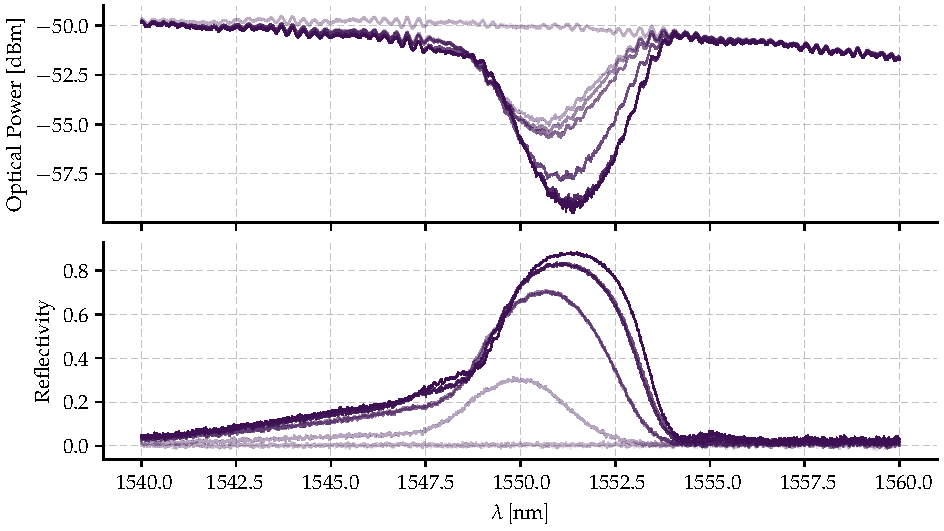
\includegraphics[width=\textwidth]{plot_time_elapsed_fbg_production_en.pdf}
	\caption{\hl{Data} %MDPI: Commas are only used for numbers with five or more digits. We removed them in four-digit numbers in the figure. Please confirm. same as other figures. Response: Confirmed. We agree with the removal of commas in four-digit numbers.
 acquired during the production of an \glsentryname{fbg} with transmission interrogation.\protect\label{fig:-34} The ripples observed in the Optical Power graphic are static spectral artifacts of the inscription setup. As shown in the Reflectivity graph, these artifacts are eliminated by the differential calculatin described in \cref{eq:-s104}.}
	
	
	
	
\end{figure}


The three resulting pairs of \glspl{fbg}, with slightly shifted reflectivity peaks to allow for differential measurement, are shown in \cref{fig:-61}. The spectral bandwidth of the fabricated \glspl{fbg} ($\approx$$\SI{3}{\nano\meter}$) was specifically selected to optimize the sensor's dynamic range. While narrower gratings would provide a steeper spectral slope (higher optical sensitivity), they would significantly restrict the linear measurement range, leading to early saturation. The chosen bandwidth ensures a monotonic response over the target range of $\pm \SI{20}{\gravity}$, with the trade-off in optical sensitivity being compensated by the gain of the electronic signal conditioning stage. Furthermore, the objective was to design the pairs so that, under zero acceleration, the crossing point between their spectra occurs in the region of steepest slope, corresponding to {50}\% of the maximum reflectivity. This configuration maximizes the effective full-scale range from an optical perspective, as will be discussed in \cref{subsection:-1}.






\subsection{Differential Optical Interrogation Circuit}

The operating principle of the accelerometer is based on the differential interrogation technique, implemented through a dual-reflection topology.
The complete optical circuit, illustrated in \cref{fig:unificada}, integrates the stabilized optical source with the three measurement channels, corresponding to the sensitive axes $x$, $y$, and $z$.
The optical source is composed of an \gls{sld} (DenseLight DL-CS5203A), whose stability is ensured by an optical isolator. The emitted light is sequentially divided: a 99:1 coupler splits a fraction of the power to a reference photodetector ($\text{PD}_{\text{ref}}$) in the $1\%$ channel to mitigate the effects of source fluctuations, while the main channel ($99\%$) is subsequently split by a 1:3 coupler, distributing the power to the three distinct outputs ($\mathbf{x}$, $\mathbf{y}$, and $\mathbf{z}$) which serve as sources for the interrogation circuits of each axis.
Each axis utilizes an identical differential interrogation circuit composed of a 50:50 coupler and a pair of \glspl{fbg} that act as differential sensors. This configuration physically implements the differential measurement method, whose conceptual basis assumes that the acceleration along an axis can be inferred directly from the strain difference between a pair of opposing \glspl{fbg}. The \gls{fbg} pairs are arranged in a ``push-pull'' configuration, where an acceleration along the sensitivity axis induces tension in one grating and simultaneous compression in the other, resulting in spectral shifts in opposite directions. The differential measurement of the separation between the Bragg peaks doubles the system's sensitivity compared to a single-grating sensor and promotes the rejection of common-mode disturbances, such as temperature fluctuations \citep{Cazo2008}. The \gls{fbg} labels in the graphics correspond to the respective \glspl{fiberSegment} illustrated in the accelerometer structure (\cref{fig:fig1}), where the term \gls{fbg} denotes the Bragg grating inscribed within the fiber core. For instance, $\text{\gls{fbg}}_1$ and $\text{\gls{fbg}}_4$ are aligned with the $x$-axis, $\text{\gls{fbg}}_8$ and $\text{\gls{fbg}}_5$ with the $y$-axis, and $\text{\gls{fbg}}_9$ and $\text{\gls{fbg}}_{12}$ with the $z$-axis, mapping directly to the specific fiber segments and connection points (e.g., $\text{\gls{fbg}}_1$ is between $\mathbf{b}_1$ and $\mathbf{m}_1$) shown in the three-dimensional diagram (\cref{fig:fig1}). All optical components used in the sensor, including \glspl{fo}, couplers, and the isolator, are of the \gls{sm} type.







\begin{figure}[H]
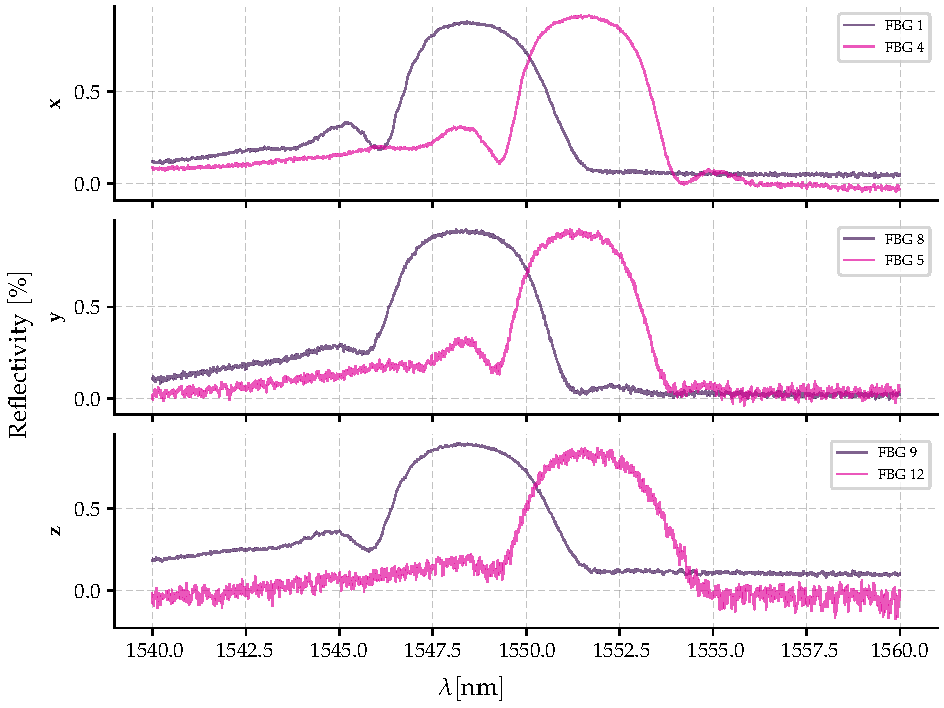
\includegraphics[width=\textwidth]{fbg_acc_4_en.pdf}
	\caption{\hl{The} %MDPI: 1. Figures should be put after their first citations, please confirm positions of all figures. Except for some in order to reduce too much space. 2. To reduce white space, we have not placed it where it is first mentioned, please confirm. Response: The figures are ok.
 \gls{fbg} labels in the graphics correspond to the respective \glspl{fiberSegment} illustrated in \cref{fig:fig1}. For instance, the curve designated \gls{fbg} 1 corresponds to the specific grating inscribed on the fiber segment $\text{\fiberSegment}_{1}$, which is defined by points $\mathbf{b}_1$ and $\mathbf{m}_1$.  \protect\label{fig:-61}}
	
	
	
\end{figure}





The reflectivity spectra of the utilized \glspl{fbg} have a bandwidth of approximately  \SI{3}{\nm}, whereas broadband sources like \glspl{sld} have spectra of approximately \SI{40}{\nm}. To analyze the interrogation equations, it is assumed that, in the operating region, the spectrum of the broadband source is approximately flat and can be modeled by:
\begin{align}
	\opticalSourceVector\left(\osaWavelength\right)= & \sldSourceAmplitude,
	\label{eq:-66}
\end{align}
where $\sldSourceAmplitude$ $\left[\text{\glsunit{sldSourceAmplitude}}\right]$ represents the amplitude of the broadband source spectrum. The optical power read by the photodetector in the dual-reflection interrogation, shown in \cref{fig:unificada}, is modeled by:
\begin{align}
	\photodetector\left(\osaWavelength\right) = & \frac{\sldSourceAmplitude}{16}\int\reflectivityVector_{2}\left(\osaWavelength\right)\reflectivityVector_{1}\left(\osaWavelength\right)\dd{\osaWavelength}.
	\label{eq:-242}
\end{align}
The terms $\reflectivityVector_{1}\left(\osaWavelength\right)$ and $\reflectivityVector_{2}\left(\osaWavelength\right)$ represent the reflectivity spectrum of the pairs for one axis as a function of wavelength $\osaWavelength$. The total power incident on the photodetector is obtained by integrating \cref{eq:-242} over the entire spectrum. The factor of 16 results from four passes of the light through the couplers.



\begin{figure}[H]
\includegraphics[page=37]{main_figure_file_en.pdf}
	\caption{Diagram of the differential optical circuit for the three accelerometer axes. The asterisk ($\boldsymbol{*}$) indicates that impedance matching was implemented to eliminate light return due to reflection at the fiber optic tip. The blue block represents a schematic cut-view of the seismic mass where the arrows indicate the connection points and sensing directions of the $\text{FBG}$ pairs. For example, on the $x$ axis, the $\text{FBG}_4$ connection is associated with the segment oriented in the $+\basex$ direction, and $\text{FBG}_1$ with the $-\basex$ direction.} \protect\label{fig:unificada}
	
	
\end{figure}



The choice of this differential intensity-based interrogation architecture, as opposed to standard \gls{wdm} approaches, is strictly driven by the requirements of embedded aerospace applications. While \gls{wdm} offers superior multiplexing density, it typically necessitates complex spectral analysis hardware—such as tunable lasers or high-resolution spectrometers—to track individual Bragg wavelengths. These devices are generally bulky, expensive, and power-intensive, making them less suitable for small-satellite or sounding rocket payloads with severe \gls{swap} constraints.

In contrast, the proposed topology converts the wavelength shift directly into an optical power variation through the spectral overlap of the FBG pairs. This allows the demodulation to be performed by a fully passive optical circuit coupled with simple photodetectors and standard operational amplifiers (as detailed in \cref{subsection:sinalConditining}). This architecture not only reduces the system's footprint and cost but also provides a high-bandwidth analog output suitable for real-time control loops, avoiding the sampling rate limitations often found in low-cost scanning interrogators.	Furthermore, this architecture offers the potential for future integration into a complete optical \gls{imu}, where the broadband light source could be shared with a \gls{ifog}, significantly optimizing the system's overall power budget and~footprint. 

\subsection{Full-Scale Range Analysis\label{subsection:-1}}

The determination of the accelerometer's full-scale range was carried out from two perspectives: the mechanical limit, related to the structural integrity of the fibers, and the optical limit, imposed by the nature of the interrogation system. The fiber segment is modeled as a linear spring with stiffness $\springStifness$, as described by \cite{Timoshenko1982}.
It is important to note that acrylate coating was mechanically stripped in the sensing region (the \gls{fiberSegment} between $\conexaoMassaSismica_{m}$ and $\conexaoBase_{m}$) prior assembly. This eliminates viscoelastic creep effects and ensures that the stiffness is governed solely by the silica cladding proprieties.
Assuming a Young's modulus for silica of $\moduloYoung=\SI{70}{\giga\pascal}$, an optical fiber diameter of $\opticalFiberDiameter=\SI{125}{\um}$, and an initial length of $\comprimentoInicialFibra=\SI{3}{\mm}$, the stiffness $\springStifness$ was calculated as:
\begin{equation}
	\springStifness=\frac{\moduloYoung\frac{\pi\opticalFiberDiameter^{2}}{4}}{\comprimentoInicialFibra}.
	\label{eq:-143}
\end{equation}
resulting in $\springStifness \approx \SI{286.3430804053197}{\kilo\newton\per\meter}$. From this value, the initial strain $\deformation_{a}$, due to the pre-tension $\preTensionAssembly$ of \SI{2}{\newton}, was determined as:
\begin{align}
	\deformation_{a}=\frac{\Delta\comprimentoInicialFibra}{\comprimentoInicialFibra} & =\frac{\preTensionAssembly}{\springStifness\comprimentoInicialFibra}=\num[round-precision=4]{0.002328209453230011}.
	\label{eq:-180}
\end{align}

For the estimation of the accelerometer's full-scale range, the linearized dynamics relationship was considered:
\begin{equation}
	\massaSismica\ddot{r}=4\springStifness\Delta\comprimentoInicialFibra.
	\label{eq:-115}
\end{equation}
in which $\massaSismica$ and $\ddot{r}$ represent the seismic mass and acceleration, respectively, and $\Delta\comprimentoInicialFibra$ is the change in length of the fiber segment. The factor $4\springStifness$ arises from the parallel combination of the fiber segments. By substituting \cref{eq:-143} into \cref{eq:-115}, the measured strain $\deformation_{m}$ can be expressed as a function of acceleration, yielding:
\begin{align}
	\deformation_{m} & =\frac{\massaSismica\ddot{r}}{\moduloYoung\pi\opticalFiberDiameter^{2}}.
	\label{eq:-178}
\end{align}

The two strain components, $\deformation_{a}$ and $\deformation_{m}$, which cause the spectral shifts, make up the total strain imposed on each fiber segment. Thus, the Bragg equation (\cref{eq:-81}) can be rewritten to provide the relationship between the change in Bragg wavelength $\Delta\wavelengthFBG$ and the strains $\deformation_{m}$ and $\deformation_{a}$:
\begin{equation}
	\frac{\Delta\wavelengthFBG}{\wavelengthFBG}=\left(1-\effectiveOpticalDeformation\right) \left(\deformation_{m}+\deformation_{a}\right) + \left(\thermalExpantionCoefficient+\thermalOpticalCoefficient\right)\Delta\temperature.
	\label{eq:-34-1}
\end{equation}
It is observed that the measured strain $\deformation_{m}$ can be positive or negative, depending on the position relative to the seismic mass and the direction of acceleration. The breaking strain of the PS1250/1500 optical fiber (without the protective jacket) is \num[round-precision=3]{0.006} \cite{Antunes2008}. Therefore, the accelerometer must operate within the strain range:
\begin{equation}
	0<\left|\deformation_{a}+\deformation_{m}\right|<\num[round-precision=3]{0.006}.
	\label{eq:-32-1}
\end{equation}
The inequality in \cref{eq:-32-1} {shows} that the total strain $\deformation_{a}+\deformation_{m}$ must remain below the \glspl{fo} breaking point and above zero strain to maintain structural integrity. In the case of  compression, {where }%EE: please check intended meaning has been retained.
$\deformation_{m}$ is negative, to avoid fiber slackness (loss of traction), it is necessary that $\deformation_{m}>-\deformation_{a}$; therefore, based on \cref{eq:-180}, $\deformation_{m}>-\num[round-precision=4]{0.002328209453230011}$. Conversely, under traction traction, the limit in \cref{eq:-32-1} dictates that $\deformation_{m}<\num[round-precision=4]{0.006}-\deformation_{a}$, resulting in $\deformation_{m}<\num[round-precision=4]{0.0037}$. Since the symmetric operational ranges  is constrained by tighter of these two limits, it is assumed $\left|\deformation_{m}\right|<\deformation_{a}$. Substituting this into to \cref{eq:-178}, the maximum allowable acceleration is:
\begin{equation}
	\left|\ddot{r}_{max}\right|<\frac{\deformation_{a}\moduloYoung\pi\opticalFiberDiameter^{2}}{\massaSismica}=\SI{672.0036772213246}{\meter\per\second\squared}\left(\SI{68.50190389615948}{\gravidade}\right).
	\label{eq:-33-1}
\end{equation}


Based on the sensor topology, where the seismic mass of $\massaSismica = \SI{16.3}{\gram}$ is suspended solely by the four optical fiber segments acting as elastic elements, the theoretical sensitivity, $\sensitivity$, can be estimated analytically. By substituting the stiffness and deformation definitions from \cref{eq:-82,eq:-115} into the Bragg relation \cref{eq:-81}, the sensitivity—defined as the ratio between the Bragg wavelength shift $\Delta \wavelengthFBG$ and the applied acceleration $\gravidade$—is given by:

\begin{equation}
	\sensitivity = \frac{\wavelengthFBG (1 - \effectiveOpticalDeformation) \massaSismica}{4 \springStifness \comprimentoInicialFibra}.
	\label{eq:-179}
\end{equation}

Considering the spring of a single fiber segment $\springStifness$ on \cref{eq:-143}, the photo-elastic coefficient of silica $\effectiveOpticalDeformation \approx 0.21$, the initial length of the \gls{fiberSegment} $\comprimentoInicialFibra=\SI{3}{\mm}$, and a center wavelength of \SI{1550}{\nano\meter}, the predicted spectral sensitivity for a single \gls{fbg} is approximately $\approx\SI{56}{\pico\meter\per\gravity}$. Due to the differential interrogation scheme employed, the effective sensitivity is doubled, resulting in a theoretical sensor sensitivity of $\approx$$\SI{112}{\pico\meter\per\gravity}$ for each axis.



Furthermore, the mechanical bandwidth is governed by the natural frequency of the mass-spring system, defined as $f_n = \frac{1}{2\pi}\sqrt{\nicefrac{4\springStifness}{\massaSismica}}$. For the implemented design parameters, the theoretical resonant frequency is approximately \SI{1.33}{\kilo\hertz}. Following standard inertial sensor design principles, the usable flat bandwidth is typically estimated as one-third of the resonant frequency to minimize amplitude distortion. Thus, the proposed sensor offers an estimated operational bandwidth of approximately \SI{440}{\hertz}, which comfortably covers the bandwidth required for tactical navigation (typically $< \SI{100}{\hertz}$). Although the dynamic response was not characterized in a vibration table due to mission integration constraints, this theoretical value aligns with the operational requirements of the interrogation system.


However, beyond the structural limits, the sensor's operating range is fundamentally restricted by the differential optical interrogation system. In this dual-reflection scheme, the detected optical power is governed by the spectral overlap between the reflections peaks of a pair of \glspl{fbg}. As shown in \cref{fig:-61}, the initial spectral separation between the peaks of the \glspl{fbg} pairs at rest is approximately $\Delta\wavelengthFBG[{}_{,sep}] \approx \SI{2.5}{\nano\meter}$.


Given the differential sensitivity of the sensor, estimated at $\approx$$\SI{112}{\pico\meter\per\gravity}$, the theoretical acceleration required to cause the spectral to crossing, leading to a loss of injectivity, can be calculated as:

\begin{equation}
	\ddot{r}_{limit} \approx \frac{\Delta\wavelengthFBG[{}_{,sep}]}{\sensitivity} \rightarrow \frac{\SI{2500}{\pico\meter}}{\SI{112}{\pico\meter\per\gravity}} \approx \SI{22.3}{\gravity}.
\end{equation}

Beyond  the range of $\approx \pm \SI{22}{g_E}$, the function relating acceleration to optical power becomes non-injective, as confirmed by the numerical simulation presented in \cref{fig:-60}. Consequently, to ensure a safe margin against measurement ambiguity and saturation, the effective full-scale range was defined as $\pm \SI{20}{g_E}$.


To evaluate the linearity performance within this theoretically defined range, a numerical simulation was performed using the experimental spectral profiles of the fabricated \glspl{fbg}, based on the theoretical model in \cref{eq:-242}. The results, presented in \cref{fig:-60}, illustrate the convolution response behavior. The greyed regions in the figure highlight the defined operational range of $\left[-\SI{20}{\gravity}, \SI{20}{\gravity}\right]$. Within this interval, the simulation confirms that the sensor maintains a monotonic and injective mapping, guaranteeing that each power measurement corresponds to a unique acceleration value. Outside this range (e.g., below approximately $-\SI{22}{\gravity}$), the relationship becomes non-injective due to the spectral crossing phenomena described above. Therefore, the simulation serves to validate the linearity of the response inside the limits imposed by the spectral separation.


\begin{figure}[H]
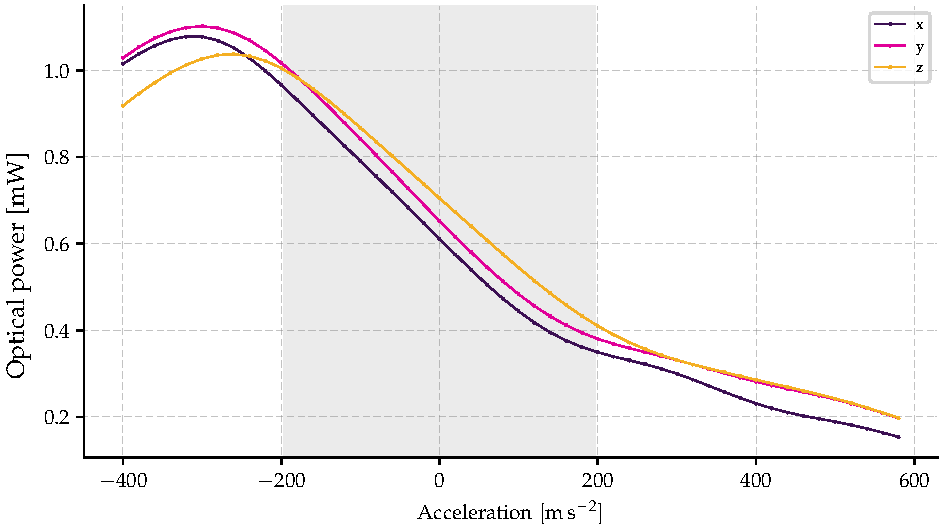
\includegraphics[width=\textwidth]{acc_4_power_vs_accel_en.pdf}
	\caption{Relationship between optical power and acceleration.\protect\label{fig:-60}}
	% \centering{}%
	\vspace{3pt}
	
\end{figure}

To quantify the adherence to a linear model, a non-linearity error analysis was performed over this full-scale range. For each axis, a linear regression was applied to the convolution results to determine the optimal slope and intercept coefficients. The non-linearity error $\epsilon_{nl}$ is defined as the maximum deviation between the simulated optical power and the linear fit, normalized by the full-scale (FS) output:

\begin{equation}
	\epsilon_{nl} = \frac{\max(|y_m - y_f|)}{\fullScale} \times 100,
	\label{eq:non_linearity}
\end{equation}
where $y_m$ represents the data points derived from the convolution and $y_f$ the corresponding values from the linear regression. This metric provides a standardized assessment of the sensor's proportional accuracy across its operating dynamic range.

\subsection{Signal Conditioning and Data Acquisition Electronics\label{subsection:sinalConditining}}

Due to the low optical power levels resulting from the differential interrogation (on the order of microwatts), a transimpedance amplifier circuit is used to convert the generated photocurrent into a measurable voltage signal. The circuit employs a low-noise \gls{ao} (OPA2727) and a photodetector with a responsivity of $\photodetectorResponsivity \approx \SI{0.9}{\ampere\per\watt}$. A first-order low-pass filter, formed by a capacitor in parallel with the feedback resistor, is implemented to limit the bandwidth and attenuate high-frequency noise.

Digital processing and data acquisition are performed by an ESP32 microcontroller, which integrates two 12-\si{\bit} \glspl{adc}. The raw \gls{adc} count values for each axis are normalized by the count from the power reference channel to compensate for source fluctuations, generating the normalized measurement vector $\overline{\measurementsStates[{}_{,i}]}$ for the $i$-th sample, according to:
\begin{equation}
	\overline{\measurementsStates[{}_{,i}]}=\frac{1}{\adcCounter[{_{\text{ref},i}}]}\left[\begin{array}{c}
			\adcCounter[{_{x,i}}] \\
			\adcCounter[{_{y,i}}] \\
			\adcCounter[{_{z,i}}]
		\end{array}\right],
	\label{eq:-14-1}
\end{equation}
where $\adcCounter[{_{\text{ref},i}}]$ is the count from the reference channel, and $\adcCounter[{_{x,i}}]$, $\adcCounter[{_{y,i}}]$, and $\adcCounter[{_{z,i}}]$ {are} the counts from each axis.

The value of the feedback resistor $\resistorTransimpedancia_{\imath}$ for the $\imath$-th axis can be sized to obtain an output voltage of $\transimpedanceTension=\SI{1.5}{\volt}$ for a given incident optical power level $\photodetector_{\imath}$, and is given by	$\resistorTransimpedancia[{_{\imath}}]=\photodetector_{\imath}\cdot\nicefrac{\transimpedanceTension}{\,\photodetectorResponsivity}$. Meanwhile, the capacitor is determined by $\capacitorFiltroPassaBaixa[{}_{ \imath}]=\left({2\pi\cdot\frequenciaCorteFiltroPassaBaixa\cdot\resistorTransimpedancia_{\imath}}\right)^{-1}.$

For the sensor's benchtop characterization, particularly the bias instability analysis via Allan Deviation, a data acquisition setup was implemented. This system combined an analog low-pass filter, with a cutoff frequency ($\frequenciaCorteFiltroPassaBaixa$) designed at $\approx\SI{1}{\hertz}$, and a digital sampling rate ($\frequenciaAmostragem$) of $\SI{100}{\hertz}$.

This configuration is ideal for static noise characterization. The analog filter serves as a robust anti-aliasing filter, maximizing the attenuation of high-frequency noise. This is particularly effective at rejecting specific disturbances common in a laboratory environment, such as low-frequency building microvibrations and thermal chamber compressor noise. Concurrently, the \SI{100}{\hertz} sampling rate provides significant oversampling of the signal band of interest ($\frequenciaAmostragem\gg2\frequenciaCorteFiltroPassaBaixa$).



This combination ensures the quasi-static signal is digitized with high fidelity. While this filtering attenuates high-frequency white noise, thereby improving the measured \gls{vrw} relative to a broader bandwidth dynamic application, it does not distort the bias instability measurement. Since the bias instability phenomenon dominates at long correlation times ($\tau \gg 1/f_{c}$), it remains unaffected by the \SI{1}{\hertz} low-pass cutoff, preserving the validity of this critical tactical-grade metric.

It must be emphasized, however, that this cutoff frequency is specific to the static testing protocol. For the final application in dynamic navigation, the filter must be redesigned for a higher cutoff frequency (e.g., $\SI{50}{\hertz}$). This is necessary to avoid introducing significant phase lag into the signals of interest (aircraft rigid-body modes), which would otherwise compromise the inertial integration process.

For the thermal compensation routine, the system temperature is monitored by a digital sensor (Model AHT10, Aosong Electronics), featuring an accuracy of $\pm\SI{0.3}{\celsius}$ and resolution of $\SI{0.01}{\celsius}$. This sensor is integrated into the acquisition electronics located inside the sealed sensor housing. Since the unit is factory-calibrated and used consistently for both the calibration procedure and operational flight, any absolute bias in the temperature reading is effectively absorbed by the polynomial model's bias coefficients,  $\calibratedBiasVectorT[{}_{(k)}]$ (detailed in \cref{sec:thermal_calib_model}). Furthermore, the sensor PCB is mechanically anchored to the accelerometer's aluminum structure. This arrangement ensures that the measured temperature is representative of the optomechanical assembly's thermal equilibrium, thereby minimizing the thermal lag between the structural expansion and the compensation variable.


The development of this custom interrogation system, as opposed to using commercial off-the-shelf (COTS) interrogators, is justified by the specific requirements of the intended aerospace application. First, commercial \gls{wdm} interrogators based on spectral scanning often exhibit limited sampling rates (typically $<\SI{1}{\kilo\hertz}$ for compact units). In the vibration-rich environment of a launch vehicle, this limitation precludes the detection of high-frequency structural modes and makes the navigation data susceptible to aliasing. In contrast, the proposed custom electronics provide a continuous high-bandwidth analog output, allowing for effective anti-aliasing filtering and dynamic analysis limited only by the cutoff frequency of the transimpedance amplifier.

Furthermore, the system is designed as a fully integrated optoelectronic architecture rather than a generic sensor-reader pair. The ``interrogator'' functionality is intrinsic to the optical domain, relying on the specific spectral overlap between the sensor and reference \glspl{fbg} to perform the signal demodulation. This dedicated design philosophy allows for a drastic reduction in \gls{swap} and cost compared to general-purpose spectral analyzers, making the sensor suitable for embedding in sounding rockets and microsatellite platforms where volume and energy budget are critical constraints.

\subsection{Characterization Procedures and Calibration Model}\label{sec:calibration}

The characterization of the accelerometer involved multiple procedures to evaluate its static, dynamic, and thermal performance. Static calibration was performed using the reference field method. The sensor was mounted on a two-degree-of-freedom rotation table, allowing it to be positioned in various known orientations relative to the Earth's gravitational field. From the normalized sensor readings and the reference acceleration vectors, the 12 parameters of a linear calibration model (compensation matrix $\compensationMatrixX$ and bias vector $\calibratedBiasVector$), according to \cref{eq:-15-1}, were estimated via \gls{mmq}.
\begin{equation}
	\compensatedMeasurements[{}_{,i}]=\compensationMatrixX\overline{\measurementsStates[{}_{,i}]}+\calibratedBiasVector.
	\label{eq:-15-1}
\end{equation}

This calibration method is described in detail in the works of \cite{Silva2021,Kuncar2017}. With the parameters obtained in this step, while maintaining a constant temperature, it was possible to perform the bias instability test, presented in the next section. In \cref{sec:thermal_calib_model}, a modification of this method is presented to include thermal compensation.

\subsubsection{{Bias} Instability and Velocity Random Walk\protect\label{sec:bias_stability}}

The inherent noise in an accelerometer's measurements, when integrated to obtain velocity, results in an error that grows over time. This characteristic is quantified by the \gls{vrw} parameter, denoted as $\biasVRW$. Another crucial parameter for characterizing the long-term performance of the sensor is the {bias} instability ($\biasInstability$), which describes the slow fluctuations or drift of the mean {bias} value over time. To quantitatively estimate the $\biasVRW$ and $\biasInstability$ parameters, the \gls{avarAcrony} method was adopted.

The value of $\biasVRW$ is obtained from the Allan Deviation ($\adev$, which is the square root of the Allan Variance, computed using the \texttt{AllanTools} Python library~\citep{allantools}) for a correlation time $\tau$ of \SI{1}{\second}, given by:
\begin{align}
	\biasVRW= & 60\cdot\adev\left(\tau=\SI{1}{\s}\right)\left[\si{\m\per\s\per\sqrt{\hour}}\right].
	\label{eq:-18-1-new}
\end{align}
while the $\biasInstability$ is associated with the minimum value of the Allan Deviation curve~\citep{Li2013a}.
\begin{equation}
	\biasInstability=\frac{\left.\adev\right|_{\frac{\partial\sigma}{\partial\tau}=0}\times{10}^{3}}{\num{0.66428}\times\num{9.81}}\left[\si{\milli\gravity}\right].
	\label{eq:-19-1-new}
\end{equation}

For the bias instability assessment, the sensor was kept at rest inside a thermal chamber (\cref{fig:camaraTermica}) at a controlled temperature of $\SI{23.4}{\celsius}$. The data were transmitted via {Bluetooth} and stored on a computer for post-processing. For the Allan variance analysis, the last six hours of acquisition were considered to ensure the sensor was in thermal equilibrium.

\begin{figure}[H]
\includegraphics[page=3, width=0.45\textwidth]{ipe_images_english.pdf}
	\caption{Accelerometer inside a thermal chamber for a static temperature test without attitude variation.\label{fig:camaraTermica}}
	
	
\end{figure}

\subsubsection{Calibration Model with Thermal Compensation}\label{sec:thermal_calib_model}

The linear model (\cref{eq:-15-1}), although straightforward to implement, does not account for temperature effects. Although the differential topology has the potential to mitigate common-mode thermal disturbances in the sensing element, the overall system performance remains susceptible to temperature variations in peripheral optical components. The response of passive components, such as optical couplers, exhibits thermal dependence, with variations in insertion loss and coupling ratio \citep{Chovan2011, Bednarek2016}. Additionally, optical sources like the \gls{sld} show power and wavelength variations with temperature \citep{Agrawal2002}. These systemic instabilities can manifest as {bias} and scale factor errors, reinforcing the need for a calibration model that actively compensates for the thermal dependence of the entire measurement chain.

To compensate for these errors, a polynomial calibration model with degree $n$ is proposed, which extends the linear model by incorporating temperature-dependent terms. The relationship between the reference measurement ($\compensatedMeasurements$) and the normalized raw measurement ($\overline{\measurementsStates}$) is modeled as:
\begin{equation}
	\compensatedMeasurements = \sum_{k=0}^{n} \left( \compensationMatrixXT[{}_{(k)}] \temperature^k \right) \overline{\measurementsStates} + \sum_{k=0}^{n} \left( \calibratedBiasVectorT[{}_{(k)}] \temperature^k \right).
	\label{eq:thermal_calib_model_poly}
\end{equation}

The choice of a polynomial structure of order $n$ (where $n > 1$) is physically justified by the aggregate behavior of the optoelectronic chain. While the thermal response of the \gls{fbg} sensor itself is dominated by the linear thermo-optic coefficient of silica $\thermalExpantionCoefficient$ ($\approx$$8.6 \times 10^{-6} / ^\circ $C) over the tested range, the interrogation system introduces significant non-linear dependencies. Specifically, the broadband \gls{sld} source exhibits a temperature-dependent wavelength drift and spectral shape variation (typically Gaussian). Since the measurement principle relies on the convolution of this source spectrum with the \gls{fbg} reflection profiles (as detailed in \cref{eq:-242}), a linear shift in temperature results in a non-linear variation in the integrated optical power. Furthermore, the splitting ratio of the optical couplers and the responsivity of the photodetectors also exhibit thermal sensitivities. Consequently, the polynomial coefficients $\compensationMatrixXT[{}_{(k)}] \temperature^k $ and $\calibratedBiasVectorT[{}_{(k)}] \temperature^k$ for $k \ge 2$ in \cref{eq:thermal_calib_model_poly}  act as lumped parameters to compensate for these combined systemic non-linearities, which cannot be corrected by a simple bias and scale factor adjustment.

The fundamental difference between the calibration model defined in \cref{eq:thermal_calib_model_poly} and the linear approach of \cref{eq:-15-1} lies in the explicit inclusion of thermal effects. Temperature dependence is incorporated into the scale factor matrix through the term $\compensationMatrixXT[{}_{(k)}] \temperature^k$, as well as into the bias vector via $\calibratedBiasVectorT[{}_{(k)}] \temperature^k$.

The model has a total of $N_p = 12(n+1)$ scalar parameters to be estimated. For this, \cref{eq:thermal_calib_model_poly} is rewritten as a linear matrix system in the form $\mathbf{G} = \mathbf{A}\mathbf{X}$. For a set of $m$ measurements collected at different orientations and temperatures, the matrices are defined as follows:
\begin{itemize}
	\item $\mathbf{G} \in \conjuntoReais^{3 \times m}$ is the matrix of reference accelerations, where each column corresponds to the vector $\mathbf{g}_i$ for measurement $i$.
	\item $\mathbf{A} \in \conjuntoReais^{3 \times 4(n+1)}$ is the parameter matrix to be estimated, containing the coefficients $\compensationMatrixXT[{}_{(k)}]$ and $\calibratedBiasVectorT[{}_{(k)}]$.
	\item $\mathbf{X} \in \conjuntoReais^{4(n+1) \times m}$ is the regressor matrix. Each column $\mathbf{X}_i$ is constructed from the raw measurement $\overline{\measurementsStates[{}_{,i}]}$ and the temperature $\temperature_i$, with the following structure:
	      \begin{equation}
		      \mathbf{X}_i = \left[
			      \overline{\measurementsStates[{}_{,i}]}^{\transpose}, \,
			      (\overline{\measurementsStates[{}_{,i}]} T_i)^{\transpose}, \,
			      \dots, \,
			      (\overline{\measurementsStates[{}_{,i}]} T_i^n)^{\transpose}, \,
			      1, \,
			      T_i, \,
			      \dots, \,
			      T_i^n
			      \right]^{\transpose}.
	      \end{equation}
\end{itemize}
\vspace{-6pt}

The parameter matrix $\mathbf{A}$ that minimizes the quadratic error, $||\mathbf{G} - \mathbf{A}\mathbf{X}||_F^2$, is found by the \gls{mmq} solution, given by:


\noindent
\begin{equation}
	\hat{\mathbf{A}} = \mathbf{G} \mathbf{X}^{\transpose} (\mathbf{X} \mathbf{X}^{\transpose})^{-1}.
	\label{eq:mmq_solution_poly_revised}
\end{equation}

The expression $||\mathbf{G} - \mathbf{A}\mathbf{X}||_F^2$ represents the squared Frobenius norm of the residual error matrix. The resulting difference matrix, $\mathbf{E}= \mathbf{G}-\mathbf{A} \mathbf{X}$, aggregates the estimation errors for all $m$ measurements and for the three axes. The Frobenius norm is defined as the square root of the sum of the squares of all matrix elements, analogous to the Euclidean norm for vectors. Therefore, minimizing the square of this norm is precisely the objective of \gls{mmq}: to find the parameter matrix $\hat{\mathbf{A}}$ that minimizes the total sum of squared errors across the entire dataset.

Conceptually, this estimation problem is equivalent to finding the affine transformation that maps the distorted ellipsoid, formed by the raw measurements at different orientations, back to the ideal sphere with a radius of $\SI{1}{\gravity}$, since gravity is used as the reference in this case. The scale factor matrix corrects the ellipsoid's distortion, and the bias ensures that the ellipsoid is centered at the origin.

Although geometric fitting methods exist \citep{Markovsky2004}, the algebraic \gls{mmq} approach was adopted here for two strategic reasons. First, its computational simplicity allows for an efficient implementation on embedded hardware \citep{Silva2021}. Second, the algebraic formalism permits a direct extension of the model to incorporate thermal dependencies, providing the foundation for the proposed comprehensive calibration model. The choice of the polynomial degree, $n$, represents a trade-off between model fidelity and the risk of overfitting.

For the thermal characterization, the calibration procedure was repeated at different controlled temperatures (\SI{16}{\celsius}, \SI{24}{\celsius}, and \SI{45}{\celsius}) using a testbed with temperature control and three-degree-of-freedom rotation. \cref{fig:dados_adquiridos_ensaio_temperatura} presents the data acquired for calibration, already normalized by the reference measurement. The test is performed by pointing one axis at a time vertically downwards and upwards. The first axis was the $\mathbf{z}$-axis, with a \SI{180}{\degree} rotation around the $\mathbf{y}$-axis. Then, the $\mathbf{x}$-axis was subjected to the same procedure, followed by the $\mathbf{y}$-axis.
\begin{figure}[H]
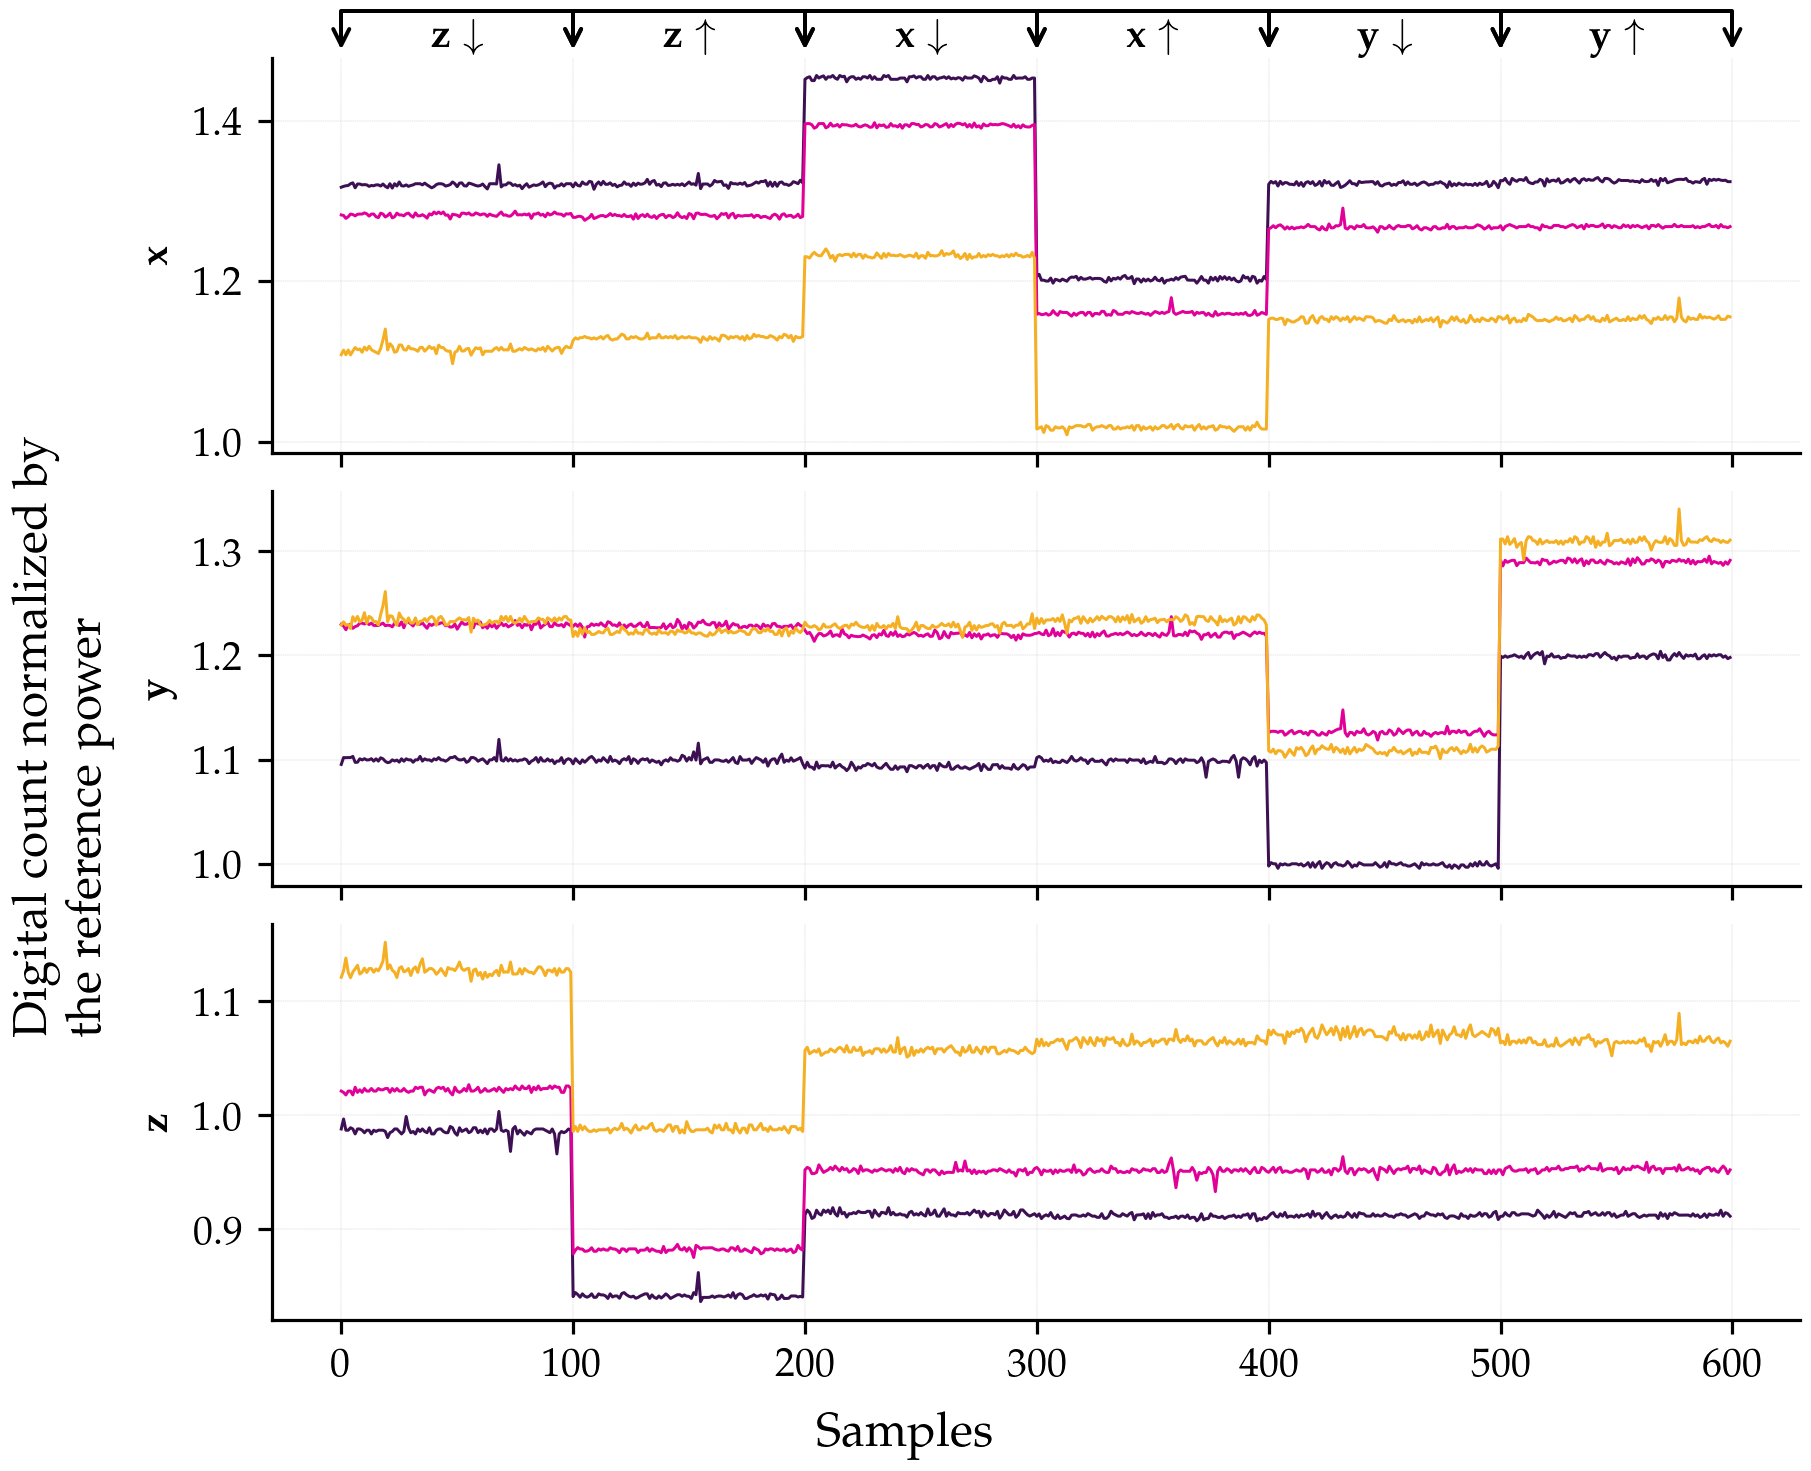
\includegraphics[width=0.9\columnwidth]{uncalibrated_data_en.png}
	\caption{\hl{Data} %MDPI: Please confirm whether an explanation of the colors needs to be added to the figure caption. Response: We add a explanation on figure label.
 acquired for calibration under controlled temperature conditions. \textcolor{blue}{The colors purple, magenta, and yellow represent \SI{16}{\celsius}, \SI{24}{\celsius}, and \SI{45}{\celsius}, respectively}. At the top of the graph, the axis that is parallel to the gravity vector is indicated, where the notation $\mathbf{z}\downarrow$ signifies that  the{ respective axis ($\mathbf{z}$) is oriented downward. In this setup, the other two axes are orthogonal to gravity and, ideally, should exhibit zero measurement. However, the acquired data reveals significant cross-axis coupling effects. The subsequent section {presenting the} results demonstrates the capability of the proposed calibration method to effectively correct these parasitic effects.}}	\label{fig:dados_adquiridos_ensaio_temperatura}
\end{figure}

\vspace{12pt}






It is worth noting that, to ensure the metrological reliability required for such high-performance applications, the characterization of modern accelerometers increasingly follows standardized guidelines, such as the IEEE Std 1293-2018 \cite{IEEE1998}. However, while the aforementioned studies focus primarily on optimizing sensitivity and frequency response, a critical and often overlooked aspect is the rigorous characterization of thermal bias stability under standardized protocols. This focus is justified because the bias stability is the governing parameter during the initial alignment and `warm-up' phases of inertial navigation systems, determining the accuracy of the attitude estimation while the vehicle is stationary.

\section{Results and Discussions}\label{sec:resultados}

This section presents the experimental results of the accelerometer characterization, including the validation of the conditioning circuit, static calibration, instability analysis, and the evaluation of the thermal compensation model.


\subsection{Conditioning Circuit Characterization}

The first experimental stage consisted of validating the signal conditioning circuit. \cref{tab:-2} presents the optical power levels measured in each channel under zero acceleration conditions. Based on these values and the responsiveness of the photodetector, the resistors (\resistorTransimpedancia) and capacitors (\capacitorFiltroPassaBaixa) of the transimpedance amplifier were sized, as discussed in \cref{subsection:sinalConditining}. The commercial values used and the resulting cutoff frequency are also presented, demonstrating the circuit's compliance with the design parameters.

\begin{table}[H]
\setlength{\tabcolsep}{2.8mm}
	\caption{\hl{Measured} %MDPI: we added a line in the table. Please confirm.  Response: Confirmed.
 power values at rest and conditioning circuit components for each channel.\protect\label{tab:-2}}

	\centering{}%
	\begin{tabular}{cccccc}
		\toprule
		                    & \multirow{2}{*}{\textbf{Optical Power}\vspace{-6pt}} & \multicolumn{2}{c}{\boldmath{$\resistorTransimpedancia$} }& \multicolumn{2}{c}{\boldmath{$\capacitorFiltroPassaBaixa$}}                                                                                                       \\
		\cmidrule{3-6}
		                    &                                & \textbf{Calculated}                                     & \textbf{Used}                                             & \textbf{Calculated}                                   & \textbf{Used} \boldmath{$\left(\frequenciaCorteFiltroPassaBaixa\right)$ }\\
		\cmidrule{1-6}
		{99}{\%} & $\SI{11}{\mW}$                 &                                                &                                                  &                                              &                                                      \\
		{1}{\%}  & $\SI{101}{\uW}$                & $\SI{17,5}{\kohm}$                             & $\SI{16}{\kohm}$                                 & $\SI{7,8}{\uF}$                              & $\SI{10}{\uF}\;\left(\SI{1}{\hertz}\right)$            \\
		$\basex$            & $\SI{730}{\nano\watt}$         & \multicolumn{2}{c}{$\SI{2,4}{\Mohm}$}          & $\SI{52,4}{\nF}$                                 & $\SI{47}{\nF}\;\left(\SI{1.7}{\hertz}\right)$                                                         \\
		$\basey$            & $\SI{1,4}{\uW}$                & \multicolumn{2}{c}{$\SI{1,2}{\Mohm}$}          & $\SI{104,7}{\nF}$                                & $\SI{100}{\nF}\;\left(\SI{1.3}{\hertz}\right)$                                                        \\
		$\basez$            & $\SI{2}{\uW}$                  & $\SI{886}{\kohm}$                              & $\SI{820}{\kohm}$                                & $\SI{153,2}{\nF}$                            & \hl{$100+\SI{47}{\nF}\;\left(\SI{1.3}{\hertz}\right)$} %MDPI: Please confirm if  keep no space before. Response: Space added.
      \\
		\bottomrule
	\end{tabular}

\end{table}


\subsection{Linearity Analysis via Spectral Convolution}\label{sec:linerityAnalysisViaSpectralConvolution}

The linearity performance of the triaxial accelerometer was evaluated for the $\mathbf{x}$, $\mathbf{y}$, and $\mathbf{z}$ axes by analyzing the convolution of the \glspl{fbg} spectra, as illustrated in \cref{fig:linearity_graphic}. This analysis, based on the relationship between optical power and acceleration shown in \cref{fig:-60}, indicates that the non-linearity error remains below \SI{6.7}{\percent} of the FS for all axes within the range up to \SI{180}{\metre\per\second\squared}.


In this characterization, the $\mathbf{x}$ and $\mathbf{y}$ axes exhibited the highest deviation, reaching approximately {6.6}{\%} and {6.3}{\%} at the upper limit of the scale, respectively. Conversely, the $z$-axis demonstrated superior linear stability, presenting the lowest non-linearity error. This behavior is attributed to the inherent spectral profiles of the inscribed gratings. As observed in \cref{fig:-61}, the spectra of the six \gls{fbg} segments are not identical; variations in bandwidth, reflectivity, and side-lobe suppression ratio (SLSR) result in distinct convolution integrals for each segment. Consequently, as the acceleration increases and shifts the Bragg wavelengths, the non-uniformity of the spectral shapes introduces slight non-linearities in the power-to-acceleration mapping. Despite these variations, the results remain predictable and suitable for compensation through the calibration model described in \cref{sec:calibration}.




\begin{figure}[H]
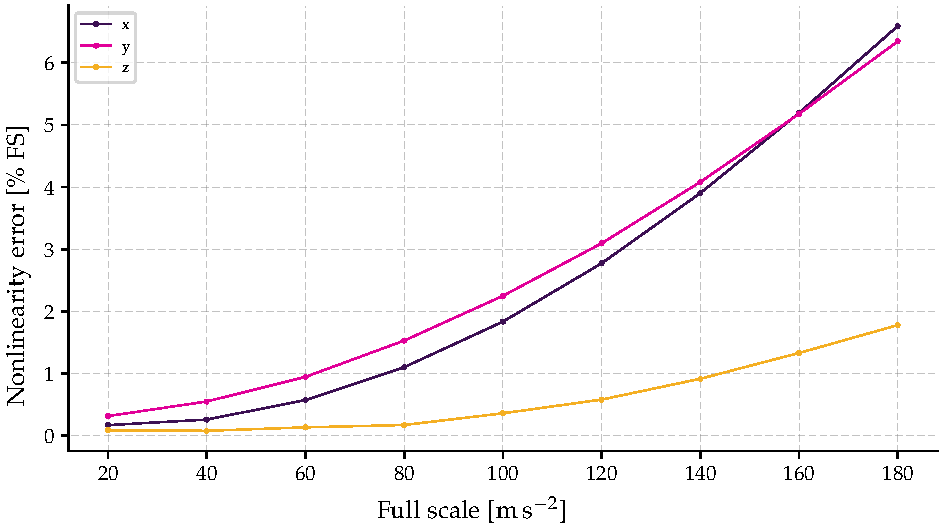
\includegraphics[width=\textwidth]{linearity_graphic_acc4_en.pdf}
	\caption{Non-linearity error as a function of the full-scale acceleration for the three orthogonal axes.\protect{\label{fig:linearity_graphic}}}
	
	 
\end{figure}






\subsection{Static Calibration at Constant Temperature}

The static calibration was performed at a temperature of \SI{23.4}{\celsius}. \Cref{fig:-64} illustrates the acquired raw dataset, the reference power, and the orientation to which the sensor was subjected. The test was conducted by rotating the sensor around the $\psiEuler$ axis and incrementing the $\thetaEuler$ angle after each full turn. In both cases, the increments were \SI{30}{\degree}. With these angles, the local gravity vector was transformed into accelerations in the sensor's fixed frame and stored in the reference measurement matrix.

The application of the reference-field calibration method to the input data and reference acceleration vectors resulted in the compensation matrix ($\compensationMatrixX$) and the bias vector ($\calibratedBiasVector$), whose values are presented in \cref{eq:-181,eq:-182}. The effectiveness of the calibration is evidenced in \cref{fig:-63}, which displays the data after applying the model. It is observed that the compensated measurements of the three axes follow the gravitational field reference, validating the linear model for a fixed operating temperature.

It is worth noting that the measurements for each axis must be normalized by the reference measurement. Thus, the elements of the $\compensationMatrixX$ matrix are dimensionless, while the terms of the $\calibratedBiasVector$ vector are in units of acceleration, $\si{\meter\per\second\squared}$.

\vspace{-6pt}
\begin{subequations}
	\label{eq:-38-1}
	\begin{align}
		\compensationMatrixX  & =\left[\begin{matrix}\num{-81.59921164779682}   & \num{2.8939750853251693} & \num{-0.7138201094423227} \\
              \num{1.5913659744157882}   & \num{77.66472852431315}  & \num{3.7542103398903106}  \\
              \num{-0.24362208758554327} & \num{1.232075406321603}  & \num{-107.65630555847483}
			                               \end{matrix}\right],\label{eq:-181}                                            \\
		\calibratedBiasVector & =\left[\begin{matrix}\num{101.0805147932936} & \num{-153.5850893944647} & \num{137.1589924872984}\end{matrix}\right]^{\transpose}.\label{eq:-182}
	\end{align}
\end{subequations}



\subsection{Bias Instability Analysis}

To quantify the sensor's long-term instability, a test was conducted with the accelerometer at rest inside a climatic chamber. \Cref{fig:-62} shows the temporal evolution of the calibrated measurements. The chamber was initially set at a temperature of $\SI{40}{\celsius}$. The internal temperature of the sensor, which started at $\SI{45}{\celsius}$, and the chamber set point were subsequently adjusted to $\SI{20}{\celsius}$. The sensor stabilized at a temperature of $\SI{23.4}{\celsius}$ after approximately $\num{7}$ h, highlighting the significant thermal inertia of the assembly. This initial high-temperature transient clearly demonstrates the sensor's temperature dependence and the limitation of the differential interrogation topology in fully compensating for temperature effects across the entire sensor structure.




\begin{figure}[H]
	 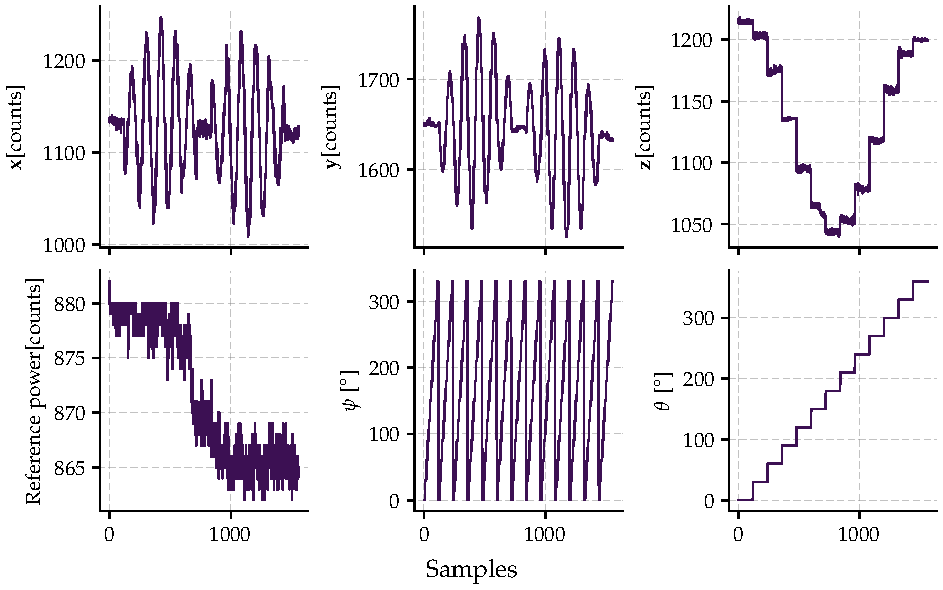
\includegraphics[width=0.95\textwidth]{collected_data_acc4_calibration_test_7_20240806_en.pdf}
	\caption{\hl{Raw} %MDPI: To reduce white space, we have not placed it where it is first mentioned, please confirm. Response: Confirmed. We agree with the new placement.
 data dataset acquired during the static calibration procedure performed at a constant temperature of $\approx$$\SI{23.4}{\celsius}$. The top row displays the uncalibrated response (in digital counts) for the $\basex$, $\basey$, and $\basez$ axes as the sensor undergoes discrete rotations. The bottom row presents the auxiliary variables: the optical reference power (used for normalization), the rotation angle $\psiEuler$ (continuous rotation around the table axis), and the inclination angle $\thetaEuler$ (discrete steps relative to gravity).\protect\label{fig:-64}}
	

\end{figure}


\vspace{-6pt}
\begin{figure}[H]
 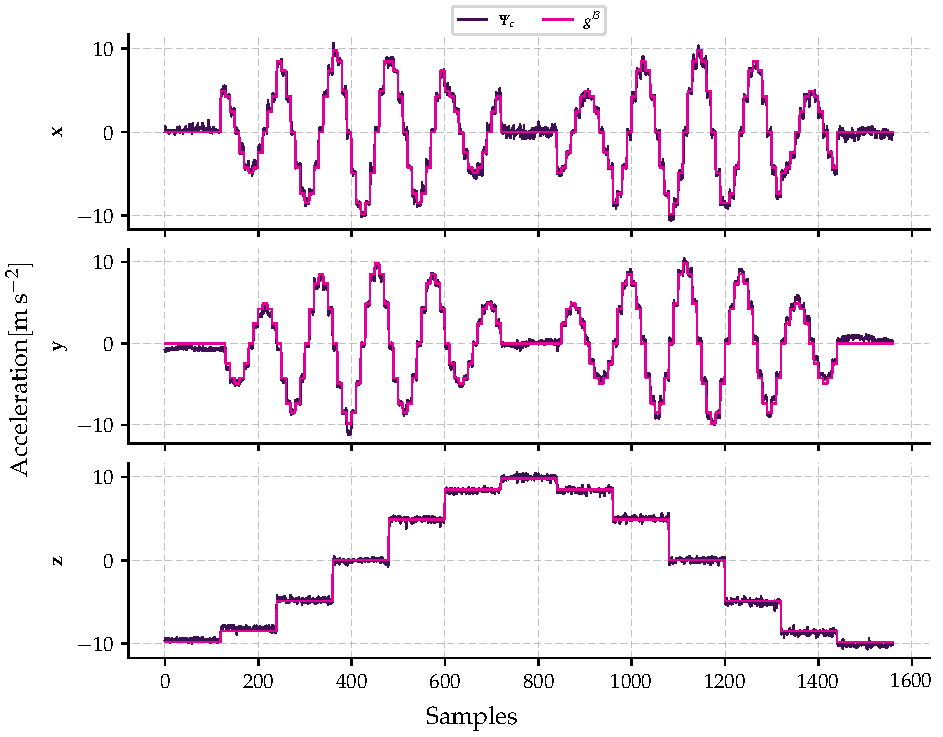
\includegraphics[width=0.95\textwidth]{calibrated_data_acc_4_calibration_test_7_20240806_en.pdf}
	\caption{\hl{Validation} %MDPI: To reduce white space, we have not placed it where it is first mentioned, please confirm. Response: Confirmed. We agree with the new placement.
 of the static calibration at $\SI{23.4}{\celsius}$. The plots compare the calibrated sensor acceleration ($\compensatedMeasurements$, purple line) against the gravitational reference field ($\vetGravidade^{\sistemaBaseSensor}$, magenta line) for the three{ orthogonal axes. The precise overlap between the measured and reference curves demonstrates the effectiveness of the estimated compensation matrix $\compensationMatrixX$ and bias vector $\calibratedBiasVector$ in correcting scale factor and misalignment errors.}}\label{fig:-63}
\end{figure}
\vspace{12pt}





The Allan Variance analysis was applied to the last six hours of data, corresponding to the period during which the sensor achieved thermal equilibrium. The \gls{adevAcrony} plot for each axis is presented in \cref{fig:-65}. From these curves, the \gls{vrw} and bias instability parameters were extracted, and their values are summarized in \cref{tab:-4}. The observed disparity in the results among the axes is likely attributable to differences in the sensitivity or the positioning of each coupler and optical component. The results, with a bias instability of less than $\SI{2}{mg}$ (milligravities), classify the sensor as tactical grade, according to the reference \cite{Lefevre2022}.




\begin{figure}[H]
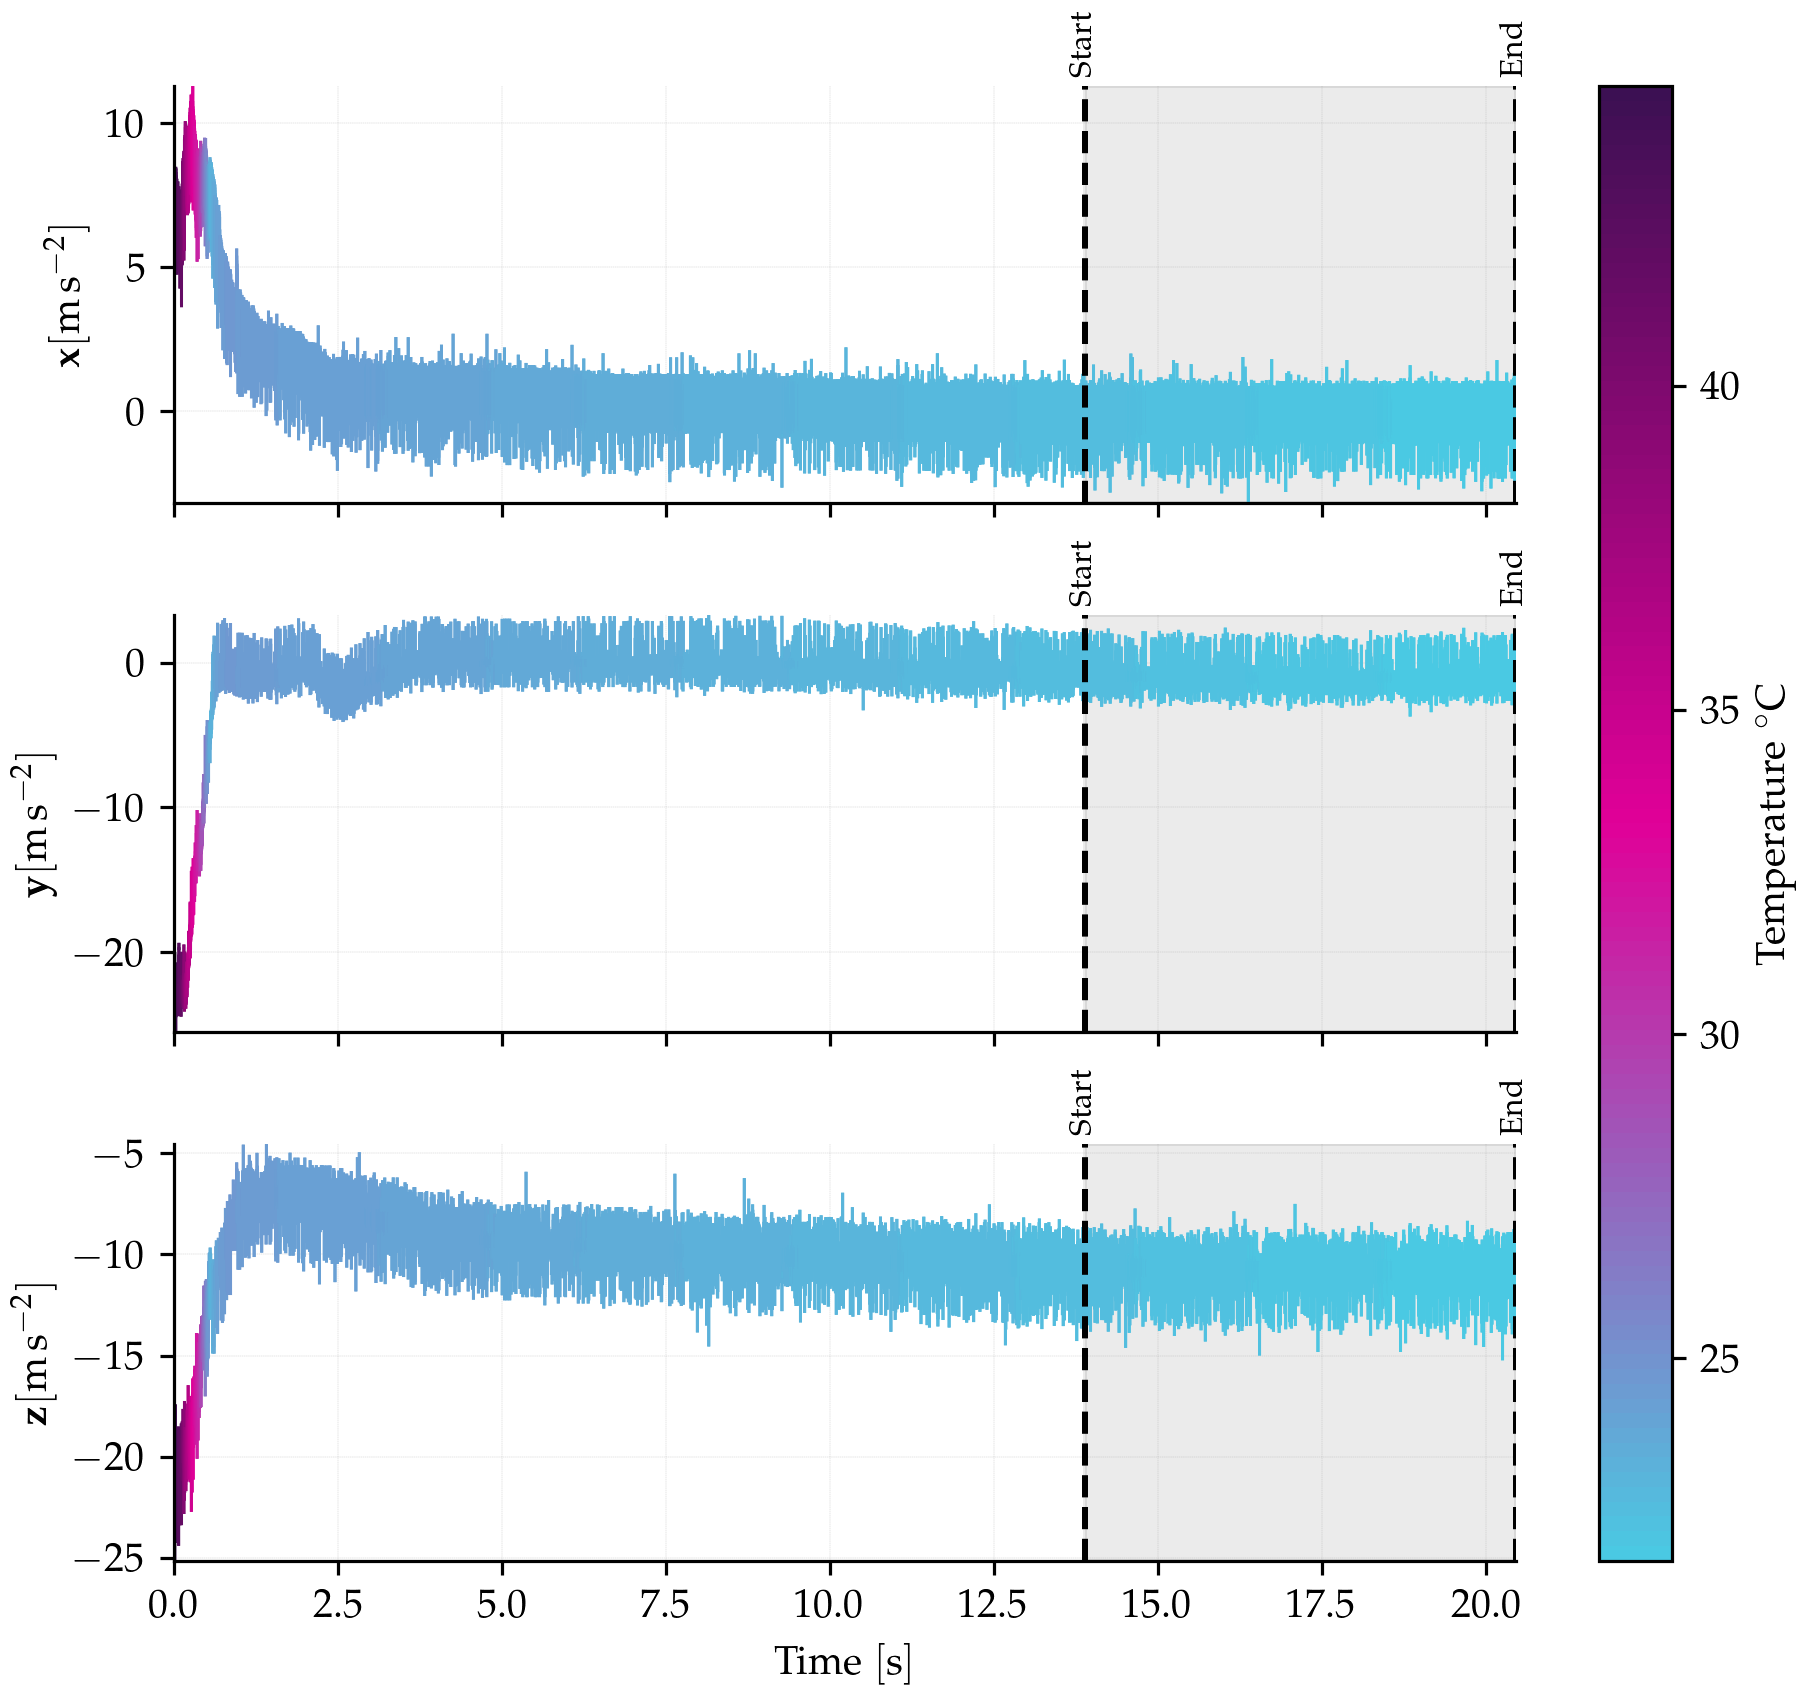
\includegraphics[width=\textwidth]{data_allan_deviation_acc_4_20240814_en.png}
	\caption{Temporal evolution of the calibrated acceleration signals during the bias instability test inside the climatic chamber. The color gradient represents the sensor's internal temperature, capturing the initial warm-up transient (from $\approx$$\SI{45}{\celsius}$ down to $\SI{23.4}{\celsius}$) and the subsequent thermal stabilization. The gray shaded region, delimited by the dashed lines 'Start' and 'End', indicates the steady-state period (thermal equilibrium) selected for the Allan Variance analysis shown in \cref{fig:-65}.\protect\label{fig:-62}}
	
		
\end{figure}




The observed disparity in the results among the axes is likely attributable to minor differences in the coupling ratios and the mounting stress of the specific fiber segments. To contextualize these results within the spectrum of inertial sensor grades, \cref{tab:grades} presents a comparisom of the accelerometer's performance with standard industry classifications \cite{Groves2007}.















\begin{figure}[H]
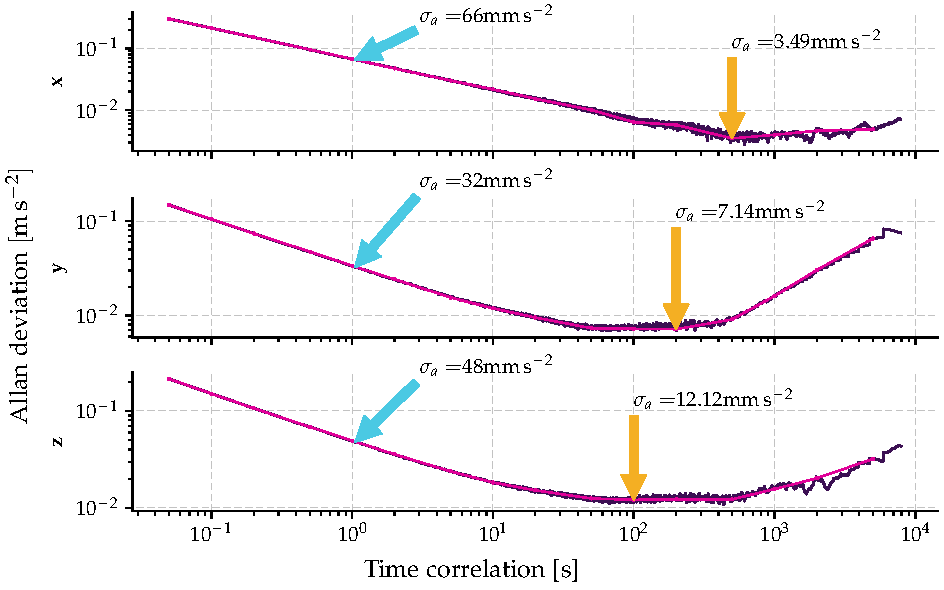
\includegraphics[width=\textwidth]{allan_deviation_acc_4_20240814_en.pdf}
	\caption{Allan Deviation (ADEV) curves computed for each axis using the steady-state data highlighted in \cref{fig:-62}. The plots identify the key stochastic noise parameters: the cyan arrows indicate the value at $\tau=\SI{1}{\second}$ (used to determine $\biasVRW$), while the orange arrows identify the curve's minimum point, corresponding to the Bias Instability ($\biasInstability$) of the sensor.\protect\label{fig:-65}}
	
		
\end{figure}
\vspace{-6pt}
\begin{table}[H]
\setlength{\tabcolsep}{11.8mm}
	\caption{\hl{Accelerometer} %MDPI: 1. Please confirm if keep bold and italic in the table. 2. please bold header in the table. Response: The bold and italic formatting has been removed as requested. The header has become bold.
 instability performance parameters.\protect\label{tab:-4}}
	\centering{}%
	\begin{tabular}{ccc}
		\toprule
		\textbf{Axis}         & \textbf{VRW} {${\left[\si{\meter\per\second\per\sqrt{{\hour}}}\right]}$} & \textbf{Bias Instability} {{$\left[\si{\milli\gravity}\right]$}} \\\midrule
		$\mathbf{x}$ & $\num{3.9594}$                                                    & $\num{0.5383}$                                 \\
		$\mathbf{y}$ & $\num{1.9444}$                                                    & $\num{1.1031}$                                 \\
		$\mathbf{z}$ & $\num{2.8702}$                                                    & $\num{1.8719}$                                 \\
		\bottomrule
	\end{tabular}
\end{table}


\vspace{-6pt}

\begin{table}[H]
\setlength{\tabcolsep}{7.1mm}

\caption{\hl{Comparison} %MDPI: Please confirm if the bold formatting in the table is necessary; if not, please remove it. Response: The bold and italic formatting has been removed as requested.
 of the developed sensor's bias instability with standard inertial navigation performance grades \cite{Groves2007}.}
\label{tab:grades}
\begin{tabular}{@{}l c c@{}}
\toprule
\textbf{Performance Grade} & \textbf{Bias Instability} & \textbf{Typical Application} \\ \midrule
Marine/Navigation & $<$$\SI{0.025}{\milli\gravity}$ & Submarines, Long-haul Aircraft \\
{Tactical} & {\SI{0.1}{}--\SI{10.0}{\milli\gravity}} & {UAVs, Short-range Missiles} \\
Automotive/Industrial & $>$$\SI{10.0}{\milli\gravity}$ & Airbags, Suspension Control \\ \midrule
{This Work} & {$<$$\SI{1.9}{\milli\gravity}$} & {Sounding Rockets/Low-LEO} \\ \bottomrule
\end{tabular}
\end{table}

As evidenced in Table \ref{tab:grades}, the achieved bias instability (ranging from \SI{0.54}{} to \SI{1.87}{\milli\gravity}) places the developed sensor within the tactical grade category. This performance level is sufficient for short-duration missions, such as sounding rockets or orbital injection phases, where GNSS denial is temporary and the integration time is limited.




\subsection{Performance of the Thermal Calibration Model}

To evaluate the sensor's performance over an operating temperature range, the calibration procedure was repeated at three temperature levels. The data in \cref{fig:dados_adquiridos_ensaio_temperatura} are concatenated in a single dataset where the first 600 points represent the data collected at $\approx$$\SI{16}{\degreeCelsius}$, the next 600 points represent the data collected in $\approx$$\SI{24}{\degreeCelsius}$, and the last 600 points represent the data collected in $\approx$$\SI{45}{\degreeCelsius}$. This new dataset is used to estimate the parameters of the polynomial model proposed in \cref{eq:thermal_calib_model_poly}. \Cref{fig:calibrated_data_with_temperature_dependency} displays the data calibrated with the thermal model. The legend indicates the polynomial degree used to model the thermal dependence of the sensor, i.e., represent the term $n$ on \cref{eq:mmq_solution_poly_revised}. It is noteworthy that, regardless of the operating temperature (indicated by distinct colors), the sensor outputs converge to the reference values, validating the effectiveness of the compensation method.

The residual nonlinearity of the sensor was quantified by analyzing the model errors for different polynomial degrees. \Cref{fig:linearity_with_respect_to_full_scale_en} shows the errors normalized by the full-scale range (\SI{20}{\gravity}). \Cref{tab:erros_residuais} presents the \gls{rmse} value of these errors. A drastic reduction in error is observed when moving from the linear model (degree 1) to the quadratic model (degree 2), especially on the $\mathbf{y}$-axis. The third-degree model offers an additional improvement, while higher degrees (4 to 6) do not show significant gains, indicating that the degree-3 model is the most efficient for describing the sensor's thermal behavior.
\begin{figure}[H]
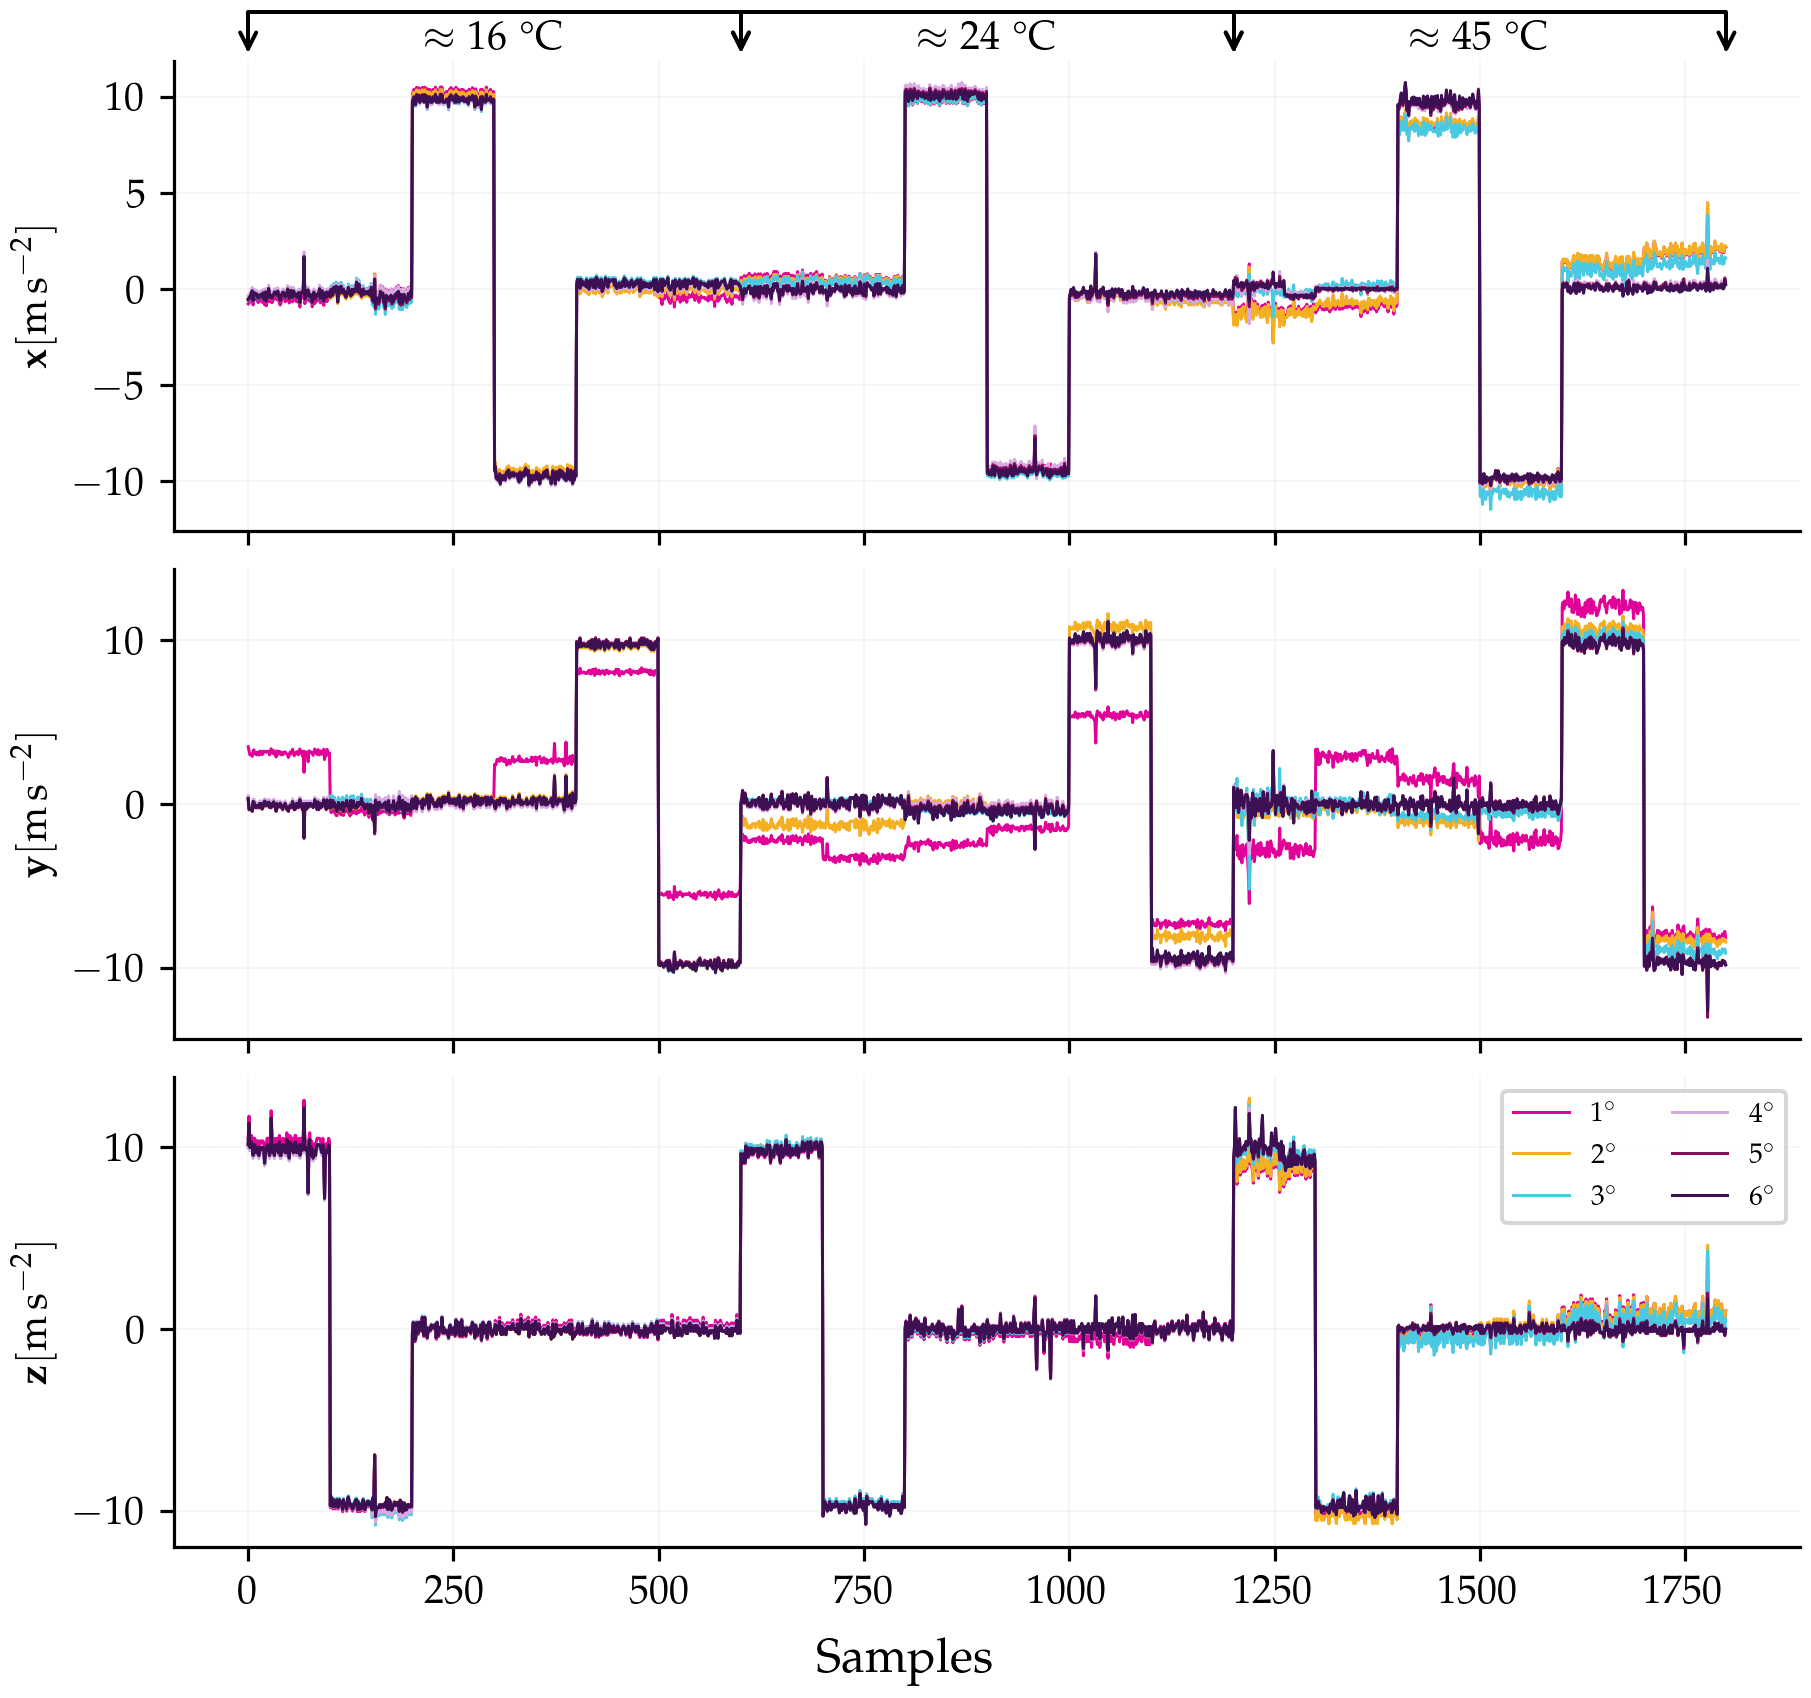
\includegraphics[width=\textwidth]{calibration_with_temperature_dependency_en.png}
	\caption{Calibrated measurements with the 3rd-degree polynomial thermal compensation model.\label{fig:calibrated_data_with_temperature_dependency}}
	
		

\end{figure}

The nonlinearity of a sensor quantifies the deviation of the provided measurement from an ideal reference model. To characterize and correct this behavior, the residual errors of the polynomial models are used to quantify the unmodeled nonlinearity. \Cref{fig:linearity_with_respect_to_full_scale_en} presents these residuals normalized by the full-scale range for models of degree 1 to 6 using \cref{eq:residuals}.

\begin{equation}
	\mathbf{e}=\frac{\left|\boldsymbol{\varPsi}_{c}-\boldsymbol{\varPsi}_{\text{ref}}\right|}{20g}.
	\label{eq:residuals}
\end{equation}

The extraction of a single value to represent the nonlinearity from this noisy data is performed by calculating a robust statistical metric, such as the \gls{rmse}, on the residuals of the lowest-degree model that effectively removes systematic trends (in this case, the  polynomial of degree 2 or 3). This \gls{rmse} value then represents the magnitude of the system's residual nonlinearity, overcoming the limitation of using the maximum absolute deviation, which would be susceptible to noise outliers.
	

		
		As discussed in \cref{sec:thermal_calib_model}, the necessity for a model of order higher than one (linear) is justified by the aggregate behavior of the optoelectronic chain. While the thermal response of the \gls{fbg} sensor itself is dominated by the linear thermo-optic coefficient of silica over this range, the interrogation system introduces non-linear dependencies.

		Specifically, the \gls{sld} exhibits a temperature-dependent wavelength drift and spectral shape variation. Since the measurement principle relies on the convolution of the source spectrum with the \gls{fbg} reflection profiles, any relative spectral shift creates a non-linear variation in the integrated optical power. Furthermore, the splitting ratio of the optical couplers and the responsivity of the photodetectors also exhibit thermal sensitivities. The second and third-order terms in \cref{eq:thermal_calib_model_poly} therefore act as lumped parameters to compensate for these combined systemic non-linearities, which cannot be corrected by a simple bias and scale factor adjustment.
		
		
		
		\begin{figure}[H]
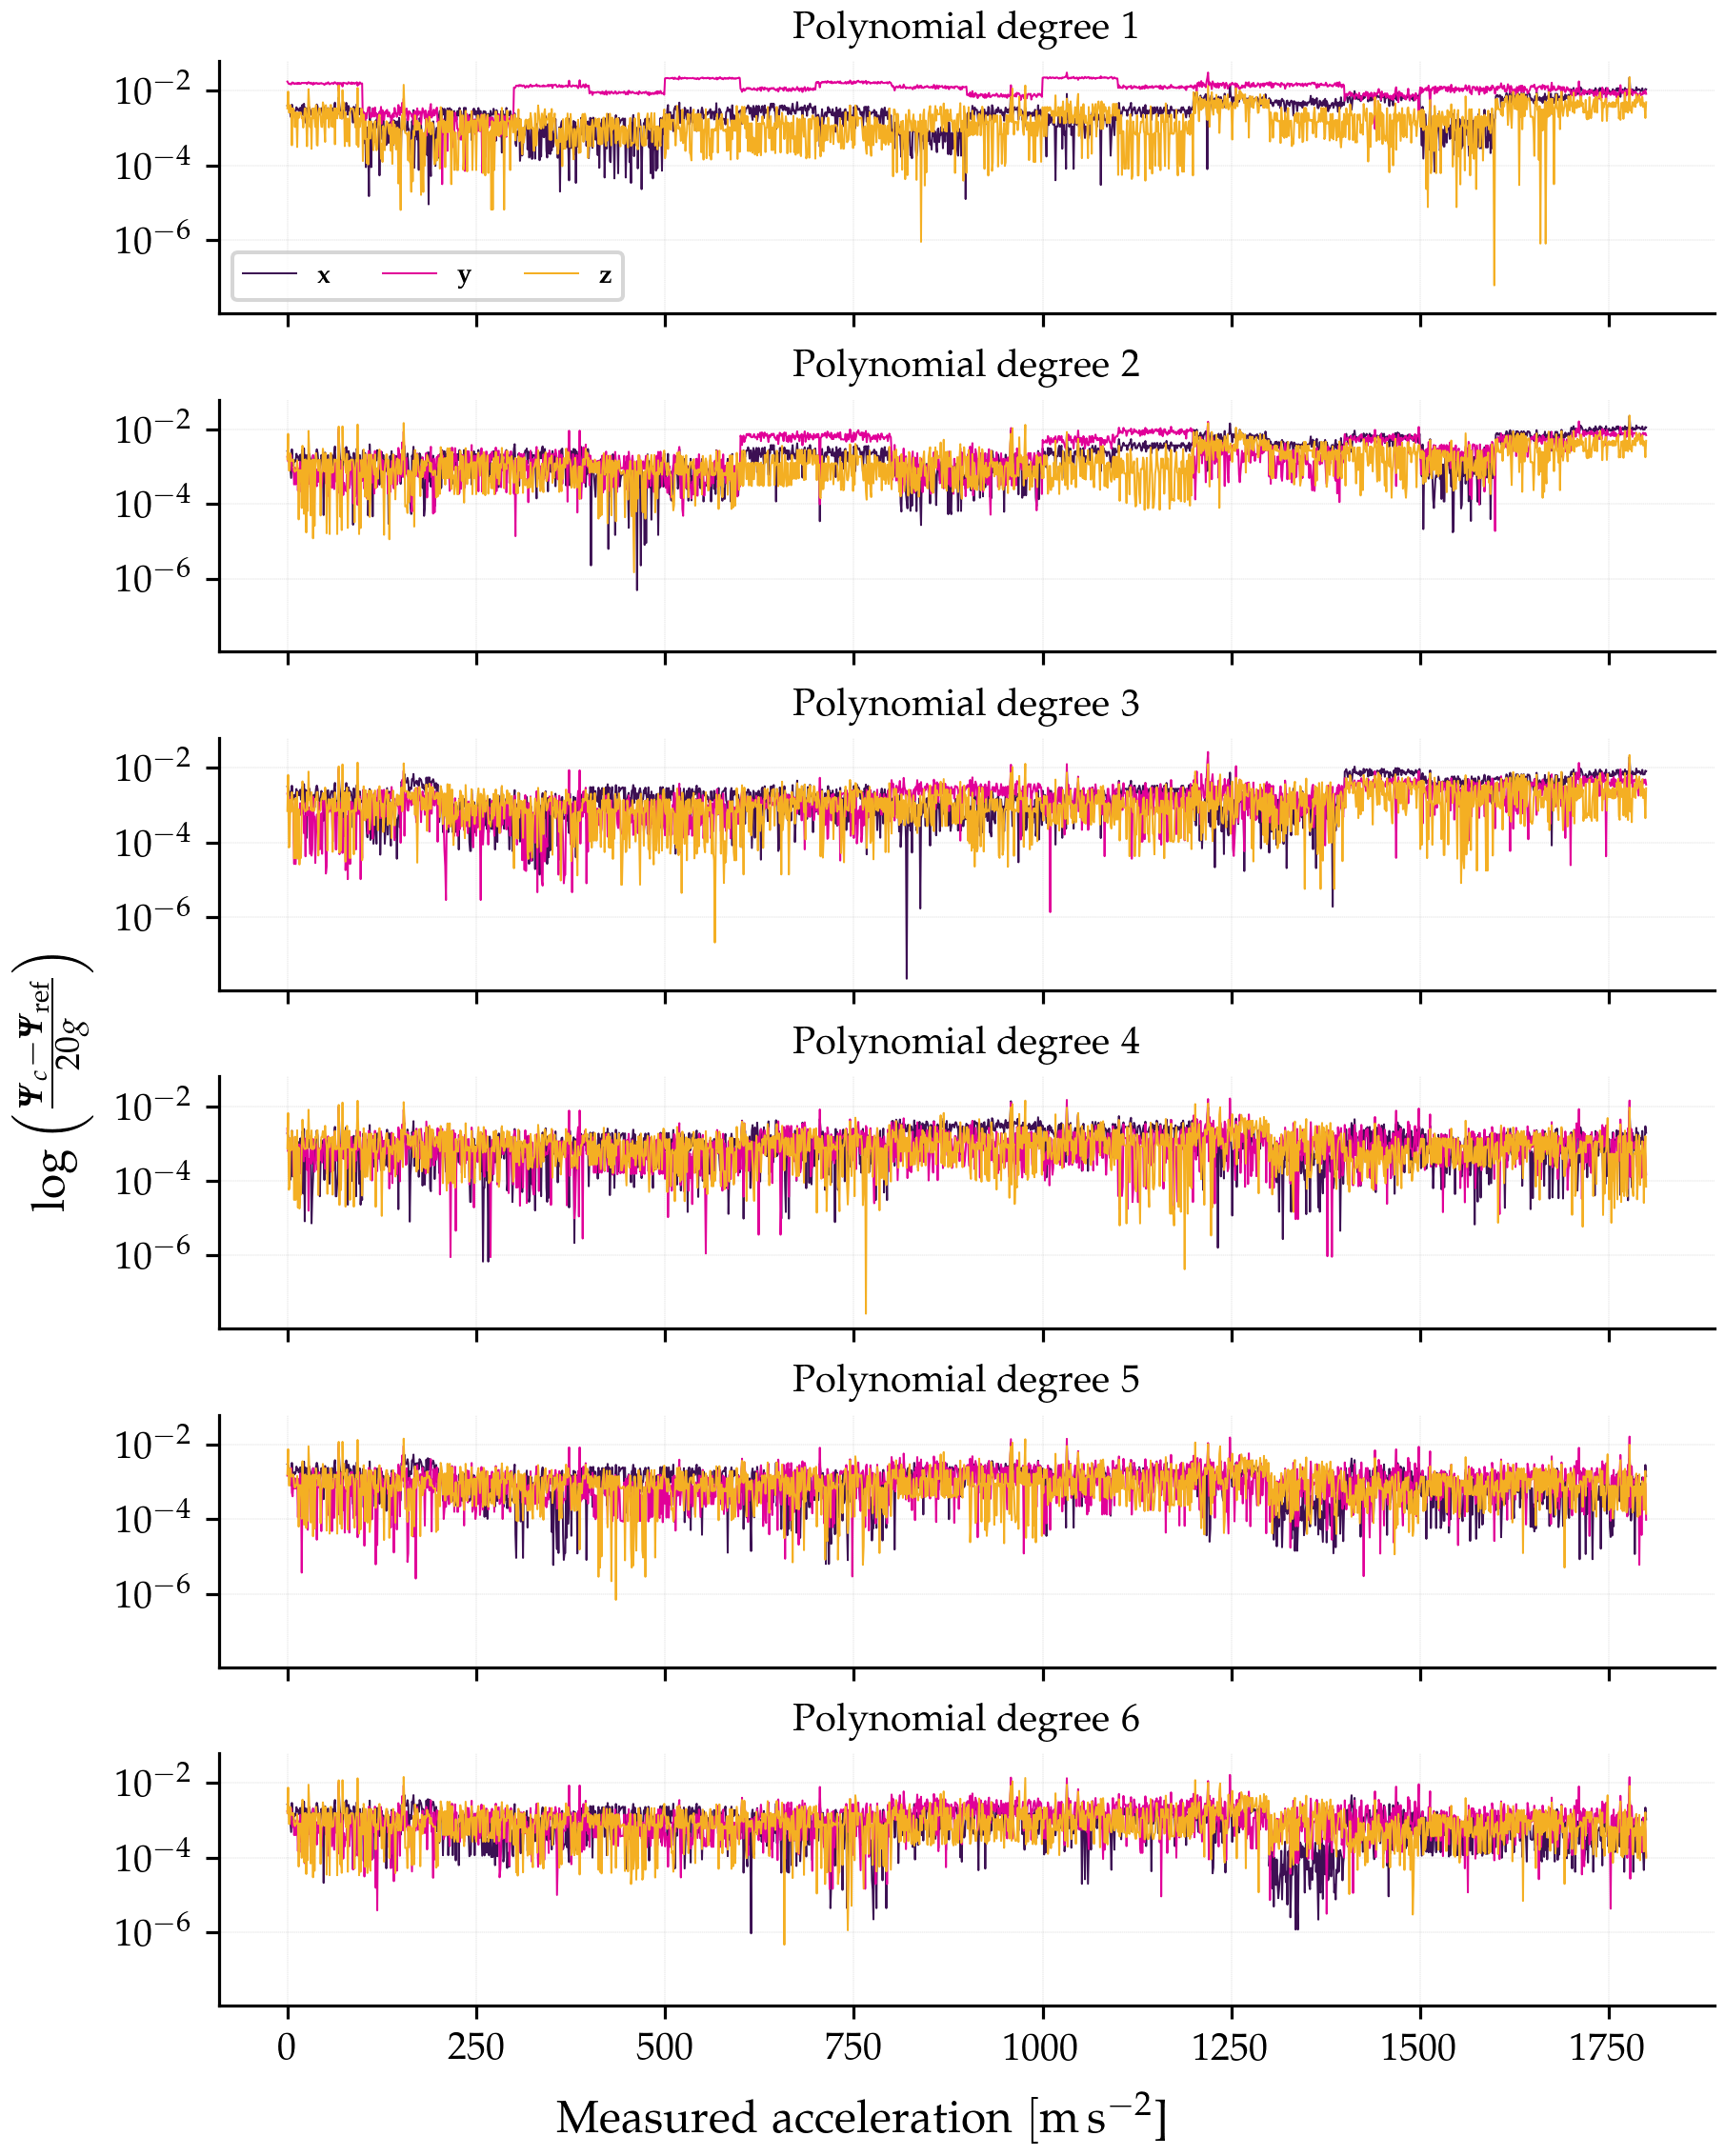
\includegraphics[width=0.82\textwidth]{linearity_with_respect_to_full_scale_en.png}
	\caption{Normalized residual errors as a function of the measured acceleration for different degrees of the polynomial thermal compensation model.\label{fig:linearity_with_respect_to_full_scale_en}}
	
	
\end{figure}
		
		
		
		
		
		
	
\begin{table}[H]
	\setlength{\tabcolsep}{9.3mm}
		\begingroup
		\sisetup{
			scientific-notation = true,
			retain-zero-exponent = false,
			round-mode = figures,
			round-precision = 1
		}
		\caption{Normalized \glsentryname{rmse} with respect {to} the degree of the polynomial model to thermal compensation.\label{tab:erros_residuais}}

		\begin{tabular}{cccc}
			\toprule
			\textbf{Degree of Poly} & $\mathbf{x}$                 & $\mathbf{y}$                & $\mathbf{z}$                \\
			\midrule
			1              & \num{0.003533759085626547  } & \num{0.03425933574279611  } & \num{0.0015855702264330274} \\
			2              & \num{0.0033627685764080458 } & \num{0.0038520831304248806} & \num{0.0013595226091497163} \\
			3              & \num{0.0022057254785727088 } & \num{0.0012661052821847072} & \num{0.000974950654430397}  \\
			4              & \num{0.0006117989085513983 } & \num{0.000551443923541311 } & \num{0.0005866014731708948} \\
			5              & \num{0.0004864567090630891 } & \num{0.000676101481339818 } & \num{0.0005882469705682579} \\
			6              & \num{0.000356307113342235  } & \num{0.0007103016927792055} & \num{0.0005679183829624561} \\
			\bottomrule
		\end{tabular}

		\endgroup
	
\end{table}


\vspace{-6pt}
\textcolor{blue}{Finally, Table \ref{tab:comparison} presents a comparison between the proposed accelerometer and state-of-the-art \gls{fbg}-based sensors reported in recent literature. While the referenced works achieve high sensitivities---often exceeding \SI{1000}{\pico\meter\per\gravity}---they are predominantly designed for seismic and structural monitoring, operating in AC frequency ranges (\SI{>0}{\hertz}) and relying on commercial spectral interrogators. In contrast, the sensor developed in this work focuses on tactical navigation requirements. It employs an embedded differential intensity interrogation system that extends the frequency response down to DC (\SI{0}{\hertz}). Furthermore, as highlighted in the table, the primary performance differentiator of the proposed architecture is the bias stability (below \SI{2}{\milli\gravity}), demonstrating its suitability for inertial navigation systems where long-term stability and \gls{swap} optimization are more critical than absolute sensitivity.}
\begin{table}[H]

\caption{\hl{Comparison} %MDPI: Please cite this table in the text and ensure that the first citation of each table appears in numerical order. Response: We have added a new paragraph citing Table 5 in the text (highlighted in blue). We also corrected a typo in the table's title ("Comparison").
 of the proposed accelerometer performance with state-of-the-art FBG-based sensors reported in recent literature.}
\label{tab:comparison}
\resizebox{\textwidth}{!}{%
\begin{tabular}{@{}l l l l l l@{}}
\toprule
\textbf{Reference} & \textbf{Topology} & \textbf{Interrogation} & \textbf{Sensitivity} & \textbf{Freq. Range} & \textbf{Key Feature/Focus} \\ \midrule
\citet{Zhou2021} & Multi-core Fiber & Micron Optics, SM130 & \SI{355}{\pm\per\gravity} & \SIrange{10}{220}{\hertz} & 3D vibration reconstruction \\
\citet{Chen2021} & Thin-cladding Cantilever & Micron Optics, SM130 & $\approx$\SI{2150}{\pm\per\gravity} & \SIrange{0.5}{30}{\hertz} & High sensitivity (Seismic) \\
\citet{Qiu2023} & Dual-Mass &  Beijing Weiyun, MWYFBG-CS800 & \SI{1194}{\pm\per\gravity} & \SIrange{1}{40}{\hertz} & Infrastructure monitoring \\
\citet{Reghuprasad2023} & Cantilever beam  & Micron Optics, SI155& \SI{433.7}{\pm\per\gravity} & \SIrange{5}{55}{\hertz} & Seismic monitoring \\
\citet{Zhang2024} & Cross-Diaphragm & \gls{fo} demodulator & \SI{590}{\pm\per\gravity} & \SIrange{0.1}{50}{\hertz} & Seismic monitoring \\
\citet{Wang2024} & Cantilever beam & \gls{fo} FBG Demodulator & \SI{1613.3}{\pm\per\gravity} & \SI{43}{\hertz} (ressonace) & Cable
force monitoring \\
\citet{Qiu2025} & Multi-flexible beam & \gls{fo} demodulator & \SI{590}{\pm\per\gravity} & \SIrange{0.05}{80}{\hertz} & Seismic monitoring \\
\citet{Liu2025} & Integrated Single-Mass  & Micron Optics, SI155& \SI{1025}{\pm\per\gravity} & \SIrange{20}{205}{\hertz} & Low cross-axis error \\
\citet{cao2025} & Integrated Single-Mass  & Ibsen, IMON 512& \SI{56.5}{\pm\per\gravity} & \SIrange{30}{80}{\hertz} & Structural health monitoring \\
\citet{VelazquezCarreon2026} & Integrated Single-Mass  & FBG demodulator (unspecified)& \SI{1730}{\pm\per\gravity} & \SIrange{1}{20}{\hertz} & Low-frequency \\ \midrule
{\hl{This Work} %MDPI: Please confirm if the bold formatting in the table is necessary; if not, please remove it. Response: The bold and italic formatting has been removed as requested.
} & {Single Seismic Mass} & {Diff. Intensity (embedded)} & {112 \si{\pico\meter\per\gravity}} (differential) & {DC---440 \si{\hertz}} & {Thermal Bias Stability (\textless 2 \si{\milli\gravity})} \\ \bottomrule
\end{tabular}%
}
\noindent{\footnotesize{{\hl{Note:} %MDPI: Please confirm if the italics are necessary; if not, please remove them. Response: The bold and italic formatting has been removed as requested.
} The sensitivity units differ due to interrogation methods (wavelength shift vs. intensity voltage output), but the key performance differentiator for navigation is the bias stability.}}

\end{table}

\section{Conclusions}\label{sec:conclusao}

This work presented the design, calibration, and performance characterization of a triaxial accelerometer based on \glspl{fbg} with differential interrogation. A comprehensive calibration methodology, which includes a polynomial model for compensating thermal effects, was proposed and experimentally validated.

The results demonstrate that the sensor has tactical-grade performance, with a bias instability of less than $\SI{1.9}{\milli\gravity}$ for all axes, validating the optomechanical architecture and the low-noise conditioning circuit. The main contribution of this work is the implementation and validation of a calibration model that efficiently corrects bias and scale factor errors induced by temperature variations. It was demonstrated that a third-order polynomial model is sufficient to reduce residual errors to a level dominated by the sensor's intrinsic noise, ensuring the accelerometer's accuracy over a wide range of operating temperatures. The obtained results qualify the sensor for applications in inertial navigation systems under different thermal conditions.

The linearity analysis, conducted via spectral convolution, revealed that the sensor maintains a predictable response within the tested range of \SI{180}{\metre\per\second\squared}, with a maximum non-linearity error of approximately {6.7}{\%} FS for the $x$-axis. It was observed that the $z$-axis presented superior linear stability compared to the others. This behavior is primarily attributed to the non-identical spectral profiles (bandwidth, reflectivity, and SLSR) of the six inscribed \glspl{fbg}, which result in distinct convolution integrals for each sensing segment. Furthermore, the triaxial sensor has potential for mechanical integrity, as the structural operating limit exceeds the current optical interrogation range.

As future work, the following are suggested: the miniaturization of the optical and electronic system; the integration of a dedicated higher-resolution \gls{adc}; and the performance of dynamic tests to characterize the device's frequency response.
%%%%%%%%%%%%%%%%%%%%%%%%%%%%%%%%%%%%%%%%%%
% \section{Materials and Methods}

% Materials and Methods should be described with sufficient details to allow others to replicate and build on published results. Please note that publication of your manuscript implicates that you must make all materials, data, computer code, and protocols associated with the publication available to readers. Please disclose at the submission stage any restrictions on the availability of materials or information. New methods and protocols should be described in detail while well-established methods can be briefly described and appropriately cited.

% Research manuscripts reporting large datasets that are deposited in a publicly avail-able database should specify where the data have been deposited and provide the relevant accession numbers. If the accession numbers have not yet been obtained at the time of submission, please state that they will be provided during review. They must be provided prior to publication.

% Interventionary studies involving animals or humans, and other studies require ethical approval must list the authority that provided approval and the corresponding ethical approval code.
% \begin{quote}
% This is an example of a quote.
% \end{quote}

% %%%%%%%%%%%%%%%%%%%%%%%%%%%%%%%%%%%%%%%%%%
% \section{Results}

% This section may be divided by subheadings. It should provide a concise and precise description of the experimental results, their interpretation as well as the experimental conclusions that can be drawn.
% \subsection{Subsection}
% \subsubsection{Subsubsection}

% Bulleted lists look like this:
% \begin{itemize}
% \item	First bullet;
% \item	Second bullet;
% \item	Third bullet.
% \end{itemize}

% Numbered lists can be added as follows:
% \begin{enumerate}
% \item	First item; 
% \item	Second item;
% \item	Third item.
% \end{enumerate}

% The text continues here.

% \subsection{Figures, Tables and Schemes}

% All figures and tables should be cited in the main text as Figure~\ref{fig1}, Table~\ref{tab1}, etc.

% \begin{figure}[H]
% %\isPreprints{\centering}{} % Only used for preprints
% 
\includegraphics[width=7 cm]{Definitions/logo-mdpi}
% \caption{This is a figure. Schemes follow the same formatting.\label{fig1}}
% \end{figure}   
% \unskip

% \begin{table}[H] 
% %\tablesize{\small}
% \caption{This is a table caption. Tables should be placed in the main text near to the first time they are~cited.\label{tab1}}
% %\isPreprints{\centering}{} % Only used for preprints
% \begin{tabularx}{\textwidth}{CCC}
% \toprule
% \textbf{Title 1}	& \textbf{Title 2}	& \textbf{Title 3}\\
% \midrule
% Entry 1		& Data			& Data\\
% Entry 2		& Data			& Data \textsuperscript{1}\\
% \bottomrule
% \end{tabularx}

% \noindent{\footnotesize{\textsuperscript{1} Tables may have a footer.}}
% \end{table}

% The text continues here (Figure~\ref{fig2} and Table~\ref{tab2}).

% % Example of a figure that spans the whole page width and with subfigures. The same concept works for tables, too.
% \begin{figure}[H]
% \centering
% %\isPreprints{}{% This command is only used for ``preprints''.
% \begin{adjustwidth}{-\extralength}{0cm}
% %} % If the paper is ``preprints'', please uncomment this parenthesis.
% \subfloat[\centering]{
\includegraphics[width=7.7cm]{Definitions/logo-mdpi}}
% \hfill
% \subfloat[\centering]{
\includegraphics[width=7.7cm]{Definitions/logo-mdpi}}\\
% \subfloat[\centering]{
\includegraphics[width=7.7cm]{Definitions/logo-mdpi}}
% \hfill
% \subfloat[\centering]{
\includegraphics[width=7.7cm]{Definitions/logo-mdpi}}
% %\isPreprints{}{% This command is only used for ``preprints''.
% \end{adjustwidth}
% %} % If the paper is ``preprints'', please uncomment this parenthesis.
% \caption{This is a wide figure. Schemes follow the same formatting. If there are multiple panels, they should be listed as: (\textbf{a}) Description of what is contained in the first panel. (\textbf{b}) Description of what is contained in the second panel. (\textbf{c}) Description of what is contained in the third panel. (\textbf{d}) Description of what is contained in the fourth panel. Figures should be placed in the main text near to the first time they are cited. A caption on a single line should be centered.\label{fig2}}
% \end{figure} 

% \begin{table}[H]
% \caption{This is a wide table.\label{tab2}}
% %\isPreprints{\centering}{% This command is only used for ``preprints''.
% 	\begin{adjustwidth}{-\extralength}{0cm}
% %} % If the paper is ``preprints'', please uncomment this parenthesis.
% %\isPreprints{\begin{tabularx}{\textwidth}{CCCC}}{% This command is only used for ``preprints''.
% 		\begin{tabularx}{\fulllength}{CCCC}
% %} % If the paper is ``preprints'', please uncomment this parenthesis.
% 			\toprule
% 			\textbf{Title 1}	& \textbf{Title 2}	& \textbf{Title 3}     & \textbf{Title 4}\\
% 			\midrule
% \multirow[m]{3}{*}{Entry 1 *}	& Data			& Data			& Data\\
% 			  	                   & Data			& Data			& Data\\
% 			             	      & Data			& Data			& Data\\
%                    \midrule
% \multirow[m]{3}{*}{Entry 2}    & Data			& Data			& Data\\
% 			  	                  & Data			& Data			& Data\\
% 			             	     & Data			& Data			& Data\\
% 			\bottomrule
% 		\end{tabularx}
% %		\isPreprints{}{% This command is only used for ``preprints''.
% 	\end{adjustwidth}
% %} % If the paper is ``preprints'', please uncomment this parenthesis.
% 	\noindent{\footnotesize{* Tables may have a footer.}}
% \end{table}

% %\begin{listing}[H]
% %\caption{Title of the listing}
% %\rule{\columnwidth}{1pt}
% %\raggedright Text of the listing. In font size footnotesize, small, or normalsize. Preferred format: left aligned and single spaced. Preferred border format: top border line and bottom border line.
% %\rule{\columnwidth}{1pt}
% %\end{listing}

% Text.

% Text.

% \subsection{Formatting of Mathematical Components}

% This is the example 1 of equation:
% \begin{linenomath}
% \begin{equation}
% a = 1,
% \end{equation}
% \end{linenomath}
% the text following an equation need not be a new paragraph. Please punctuate equations as regular text.
% %% If the documentclass option "submit" is chosen, please insert a blank line before and after any math environment (equation and eqnarray environments). This ensures correct linenumbering. The blank line should be removed when the documentclass option is changed to "accept" because the text following an equation should not be a new paragraph.

% This is the example 2 of equation:
% %\isPreprints{}{% This command is only used for ``preprints''.
% \begin{adjustwidth}{-\extralength}{0cm}
% %} % If the paper is ``preprints'', please uncomment this parenthesis.
% \begin{equation}
% a = b + c + d + e + f + g + h + i + j + k + l + m + n + o + p + q + r + s + t + u + v + w + x + y + z
% \end{equation}
% %\isPreprints{}{% This command is only used for ``preprints''.
% \end{adjustwidth}
% %} % If the paper is ``preprints'', please uncomment this parenthesis.

% %% Example of a page in landscape format (with table and table footnote).
% %\startlandscape
% %\begin{table}[H] %% Table in wide page
% %%\isPreprints{\centering}{} % This command is only used for ``preprints''.
% %\caption{This is a very wide table.\label{tab3}}
% %	\begin{tabularx}{\textwidth}{CCCC}
% %		\toprule
% %		\textbf{Title 1}	& \textbf{Title 2}	& \textbf{Title 3}	& \textbf{Title 4}\\
% %		\midrule
% %		Entry 1		& Data			& Data			& This cell has some longer content that runs over two lines.\\
% %		Entry 2		& Data			& Data			& Data\textsuperscript{1}\\
% %		\bottomrule
% %	\end{tabularx}
% %%\isPreprints{}{% This command is only used for ``preprints''.
% %	\begin{adjustwidth}{+\extralength}{0cm}
% %%} % If the paper is ``preprints'', please uncomment this parenthesis.
% %		\noindent\footnotesize{\textsuperscript{1} This is a table footnote.}
% %%\isPreprints{}{% This command is only used for ``preprints''.
% %	\end{adjustwidth}
% %%} % If the paper is ``preprints'', please uncomment this parenthesis.
% %\end{table}
% %\finishlandscape


% Please punctuate equations as regular text. Theorem-type environments (including propositions, lemmas, corollaries etc.) can be formatted as follows:
% %% Example of a theorem:
% \begin{Theorem}
% Example text of a theorem.
% \end{Theorem}

% The text continues here. Proofs must be formatted as follows:

% %% Example of a proof:
% \begin{proof}[Proof of Theorem 1]
% Text of the proof. Note that the phrase ``of Theorem 1'' is optional if it is clear which theorem is being referred to.
% \end{proof}
% The text continues here.

% %%%%%%%%%%%%%%%%%%%%%%%%%%%%%%%%%%%%%%%%%%
% \section{Discussion}

% Authors should discuss the results and how they can be interpreted from the perspective of previous studies and of the working hypotheses. The findings and their implications should be discussed in the broadest context possible. Future research directions may also be highlighted.

% %%%%%%%%%%%%%%%%%%%%%%%%%%%%%%%%%%%%%%%%%%
% \section{Conclusions}

% This section is not mandatory, but can be added to the manuscript if the discussion is unusually long or complex.

% %%%%%%%%%%%%%%%%%%%%%%%%%%%%%%%%%%%%%%%%%%
% \section{Patents}

% This section is not mandatory, but may be added if there are patents resulting from the work reported in this manuscript.

%%%%%%%%%%%%%%%%%%%%%%%%%%%%%%%%%%%%%%%%%%
\vspace{6pt}

%%%%%%%%%%%%%%%%%%%%%%%%%%%%%%%%%%%%%%%%%%
%% optional
%\supplementary{The following supporting information can be downloaded at:  \linksupplementary{s1}, Figure S1: title; Table S1: title; Video S1: title.}

% Only for journal Methods and Protocols:
% If you wish to submit a video article, please do so with any other supplementary material.
% \supplementary{The following supporting information can be downloaded at: \linksupplementary{s1}, Figure S1: title; Table S1: title; Video S1: title. A supporting video article is available at doi: link.}

% Only used for preprtints:
% \supplementary{The following supporting information can be downloaded at the website of this paper posted on \href{https://www.preprints.org/}{Preprints.org}.}

% Only for journal Hardware:
% If you wish to submit a video article, please do so with any other supplementary material.
% \supplementary{The following supporting information can be downloaded at: \linksupplementary{s1}, Figure S1: title; Table S1: title; Video S1: title.\vspace{6pt}\\
%\begin{tabularx}{\textwidth}{lll}
%\toprule
%\textbf{Name} & \textbf{Type} & \textbf{Description} \\
%\midrule
%S1 & Python script (.py) & Script of python source code used in XX \\
%S2 & Text (.txt) & Script of modelling code used to make Figure X \\
%S3 & Text (.txt) & Raw data from experiment X \\
%S4 & Video (.mp4) & Video demonstrating the hardware in use \\
%... & ... & ... \\
%\bottomrule
%\end{tabularx}
%}
\newcommand{\roney}{R.D.S.}%
\newcommand{\sakamoto}{J.M.S.S.}%
%%%%%%%%%%%%%%%%%%%%%%%%%%%%%%%%%%%%%%%%%%
\authorcontributions{Conceptualization, R.D.d.S. and \sakamoto; methodology, R.D.d.S. and \sakamoto; software, R.D.d.S.; validation, R.D.d.S. and \sakamoto; formal analysis, R.D.d.S.; investigation, R.D.d.S.; resources, \sakamoto; data curation, R.D.d.S.; writing---original draft preparation, R.D.d.S.; writing---review and editing, \sakamoto; visualization, R.D.d.S.; supervision, \sakamoto; project administration, \sakamoto; funding acquisition, \sakamoto~All authors have read and agreed to the published version of the manuscript.}%lease turn to the  \href{http://img.mdpi.org/data/contributor-role-instruction.pdf}{CRediT taxonomy} for the term explanation. Authorship must be limited to those who have contributed substantially to the work~reported.}

\funding{This study was financed by the Brazilian agency Financiadora de Estudos e Projetos (FINEP) under agreement 01.20.0207.00 and in part by the Coordenação de Aperfeiçoamento de Pessoal de Nível Superior-Brasil (CAPES)-Finance Code 001.}
%Please add: ``This research received no external funding'' or ``This research was funded by NAME OF FUNDER grant number XXX.'' and  and ``The APC was funded by XXX''. Check carefully that the details given are accurate and use the standard spelling of funding agency names at \url{https://search.crossref.org/funding}, any errors may affect your future funding.}

\institutionalreview{Not applicable.}
%In this section, you should add the Institutional Review Board Statement and approval number, if relevant to your study. You might choose to exclude this statement if the study did not require ethical approval. Please note that the Editorial Office might ask you for further information. Please add “The study was conducted in accordance with the Declaration of Helsinki, and approved by the Institutional Review Board (or Ethics Committee) of NAME OF INSTITUTE (protocol code XXX and date of approval).” for studies involving humans. OR “The animal study protocol was approved by the Institutional Review Board (or Ethics Committee) of NAME OF INSTITUTE (protocol code XXX and date of approval).” for studies involving animals. OR “Ethical review and approval were waived for this study due to REASON (please provide a detailed justification).” OR “Not applicable” for studies not involving humans or animals.}

\informedconsent{Not applicable.}%{Any research article describing a study involving humans should contain this statement. Please add ``Informed consent was obtained from all subjects involved in the study.'' OR ``Patient consent was waived due to REASON (please provide a detailed justification).'' OR ``Not applicable'' for studies not involving humans. You might also choose to exclude this statement if the study did not involve humans.

% Written informed consent for publication must be obtained from participating patients who can be identified (including by the patients themselves). Please state ``Written informed consent has been obtained from the patient(s) to publish this paper'' if applicable.}

\dataavailability{\hl{~}\textcolor{blue}{The data are available on \url{https://doi.org/10.5281/zenodo.18825983}, accessed on 1 March 2026.}} %MDPI: We encourage all authors of articles published in MDPI journals to share their research data. In this section, please provide details regarding where data supporting reported results can be found, including links to publicly archived datasets analyzed or generated during the study. Where no new data were created, or where data is unavailable due to privacy or ethical restrictions, a statement is still required. Suggested Data Availability Statements are available in section ``MDPI Research Data Policies'' at \url{https://www.mdpi.com/ethics}.} Response: We have updated the Data Availability Statement to include the Zenodo repository link containing all the datasets supporting this work.



% Only for journal Drones
%\durcstatement{Current research is limited to the [please insert a specific academic field, e.g., XXX], which is beneficial [share benefits and/or primary use] and does not pose a threat to public health or national security. Authors acknowledge the dual-use potential of the research involving xxx and confirm that all necessary precautions have been taken to prevent potential misuse. As an ethical responsibility, authors strictly adhere to relevant national and international laws about DURC. Authors advocate for responsible deployment, ethical considerations, regulatory compliance, and transparent reporting to mitigate misuse risks and foster beneficial outcomes.}

% Only for journal Nursing Reports
%\publicinvolvement{Please describe how the public (patients, consumers, carers) were involved in the research. Consider reporting against the GRIPP2 (Guidance for Reporting Involvement of Patients and the Public) checklist. If the public were not involved in any aspect of the research add: ``No public involvement in any aspect of this research''.}
%
%% Only for journal Nursing Reports
%\guidelinesstandards{Please add a statement indicating which reporting guideline was used when drafting the report. For example, ``This manuscript was drafted against the XXX (the full name of reporting guidelines and citation) for XXX (type of research) research''. A complete list of reporting guidelines can be accessed via the equator network: \url{https://www.equator-network.org/}.}
%
%% Only for journal Nursing Reports
%\useofartificialintelligence{Please describe in detail any and all uses of artificial intelligence (AI) or AI-assisted tools used in the preparation of the manuscript. This may include, but is not limited to, language translation, language editing and grammar, or generating text. Alternatively, please state that “AI or AI-assisted tools were not used in drafting any aspect of this manuscript”.}

\acknowledgments{During the preparation of this work, the authors used Gemini (Google) in order to improve grammatical accuracy. The authors have reviewed and edited the output and take full responsibility for the content of this publication.}


\conflictsofinterest{The authors declare no conflicts of interest. % Declare conflicts of interest or state ``The authors declare no conflicts of interest.'' Authors must identify and declare any personal circumstances or interest that may be perceived as inappropriately influencing the representation or interpretation of reported research results. Any role of the funders in the design of the study; in the collection, analyses or interpretation of data; in the writing of the manuscript; or in the decision to publish the results must be declared in this section. If there is no role, please state ``The funders had no role in the design of the study; in the collection, analyses, or interpretation of data; in the writing of the manuscript; or in the decision to publish the results''.}
}
%%%%%%%%%%%%%%%%%%%%%%%%%%%%%%%%%%%%%%%%%%
%% Optional

%% Only for journal Encyclopedia
%\entrylink{The Link to this entry published on the encyclopedia platform.}

% \abbreviations{Abbreviations}{
% The following abbreviations are used in this manuscript:\\

% \noindent 
% \begin{tabular}{@{}ll}
% MDPI & Multidisciplinary Digital Publishing Institute\\
% DOAJ & Directory of open access journals\\
% TLA & Three letter acronym\\
% LD & Linear dichroism
% \end{tabular}
% }


%%%%%%%%%%%%%%%%%%%%%%%%%%%%%%%%%%%%%%%%%%
%% Optional
\appendixtitles{no} % Leave argument "no" if all appendix headings stay EMPTY (then no dot is printed after "Appendix A"). If the appendix sections contain a heading then change the argument to "yes".
\appendixstart
\appendix
% \section[\appendixname~\thesection]{}
% \subsection[\appendixname~\thesubsection]{}
% The appendix is an optional section that can contain details and data supplemental to the main text---for example, explanations of experimental details that would disrupt the flow of the main text but nonetheless remain crucial to understanding and reproducing the research shown; figures of replicates for experiments of which representative data are shown in the main text can be added here if brief, or as Supplementary Data. Mathematical proofs of results not central to the paper can be added as an appendix.

% \begin{table}[H] 
% \caption{This is a table caption.\label{tab5}}
% %\newcolumntype{C}{>{\centering\arraybackslash}X}
% \begin{tabularx}{\textwidth}{CCC}
% \toprule
% \textbf{Title 1}	& \textbf{Title 2}	& \textbf{Title 3}\\
% \midrule
% Entry 1		& Data			& Data\\
% Entry 2		& Data			& Data\\
% \bottomrule
% \end{tabularx}
% \end{table}

% \section[\appendixname~\thesection]{}
% All appendix sections must be cited in the main text. In the appendices, Figures, Tables, etc. should be labeled, starting with ``A''---e.g., Figure A1, Figure A2, etc.

%%%%%%%%%%%%%%%%%%%%%%%%%%%%%%%%%%%%%%%%%%
%\isPreprints{}{% This command is only used for ``preprints''.
\begin{adjustwidth}{-\extralength}{0cm}
	%} % If the paper is ``preprints'', please uncomment this parenthesis.
	%\printendnotes[custom] % Un-comment to print a list of endnotes

	\reftitle{References}

	% Please provide either the correct journal abbreviation (e.g. according to the “List of Title Word Abbreviations” http://www.issn.org/services/online-services/access-to-the-ltwa/) or the full name of the journal.
	% Citations and References in Supplementary files are permitted provided that they also appear in the reference list here. 

	%=====================================
	% References, variant A: external bibliography
	%=====================================
	% \bibliography{your_external_BibTeX_file}
\begin{thebibliography}{999}

\bibitem[El-Sheimy and Youssef(2020)]{elsheimy2020}
El-Sheimy, N.; Youssef, A.
\newblock Inertial sensors technologies for navigation applications: State of the art and future trends.
\newblock {\em Satell. Navig.} {\bf 2020}, {\em 1},~2.

\bibitem[Borodacz and Szczepa{\'n}ski(2024)]{borodacz2024}
Borodacz, K.; Szczepa{\'n}ski, C.
\newblock GNSS denied navigation system for the manoeuvring flying objects.
\newblock {\em Aircr. Eng. Aerosp. Technol.} {\bf 2024}, {\em 96},~63--72.

\bibitem[Alghamdi et~al.(2025)Alghamdi, Alahmari, Yonbawi, Alsaleem, Ateeq, and Almushir]{alghamdi2025}
Alghamdi, S.; Alahmari, S.; Yonbawi, S.; Alsaleem, K.; Ateeq, F.; Almushir, F.
\newblock Autonomous Navigation Systems in GPS-Denied Environments: A Review of Techniques and Applications.
\newblock In \emph{Proceedings of the 2025 11th International Conference on Automation, Robotics, and Applications (ICARA)}; IEEE: \hl{Piscataway, NJ, USA,} %MDPI: Newly added information. Please confirm. Same as below. Response: Confirmed.
  2025; pp. 290--299.

\bibitem[Sanjuan et~al.(2023)Sanjuan, Sinyukov, Warrayat, and Guzman]{sanjuan2023}
Sanjuan, J.; Sinyukov, A.; Warrayat, M.F.; Guzman, F.
\newblock Gyro-free inertial navigation systems based on linear opto-mechanical accelerometers.
\newblock {\em Sensors} {\bf 2023}, {\em 23},~4093.

\bibitem[Guo et~al.(2021)Guo, Chen, Xiong, Zhou, and Li]{Guo2021}
Guo, Y.; Chen, M.; Xiong, L.; Zhou, X.; Li, C.
\newblock Fiber Bragg Grating Based Acceleration Sensors: A Review.
\newblock {\em Sens. Rev.} {\bf 2021}, {\em 41},~101--122.
\newblock {\url{https://doi.org/10.1108/sr-10-2020-0243}}.

\bibitem[Kashyap(2010)]{Kashyap2010}
Kashyap, R.
\newblock {\em Fiber Bragg Gratings}; Academic Press:  \hl{Cambridge, MA, USA,} %We added the location of publisher. Please confirm. Response: confirmed.
 2010; p. 614.

\bibitem[Berkoff and Kersey(1996)]{Berkoff1996}
Berkoff, T.A.; Kersey, A.D.
\newblock {Experimental demonstration of a fiber Bragg grating accelerometer}.
\newblock {\em IEEE Photonics Technol. Lett.} {\bf 1996}, {\em 8},~1677--1679.
\newblock {\url{https://doi.org/10.1109/68.544716}}.

\bibitem[Th\'{e}riault et~al.(1996)Th\'{e}riault, Hill, Bilodeau, Johnson, Albert, Drouin, and B\'{e}liveau]{Theriault1996}
Th\'{e}riault, S.; Hill, K.O.; Bilodeau, F.; Johnson, D.C.; Albert, J.; Drouin, G.; B\'{e}liveau, A.
\newblock {High-g Accelerometer Based on an In-Fiber Bragg Grating Sensor}.
\newblock In \emph{Proceedings of the Optical Fiber Sensors}; Optica Publishing Group: \hl{Washington, DC, USA,}  1996; p. We36.
\newblock {\url{https://doi.org/10.1364/OFS.1996.We36}}.

\bibitem[Cao et~al.(2025)Cao, Liu, Liu, Lu, Li, and Liu]{cao2025}
Cao, X.; Liu, C.; Liu, Z.; Lu, C.; Li, Z.; Liu, Z.
\newblock Elastic Plate-Coupled Dual FBG Configuration Enabling High-Sensitivity Fiber-Optic Accelerometer With Wide Frequency Range.
\newblock {\em IEEE Sens. J.} {\bf 2025}, \hl{\emph{25}, 17085--17093.}

\bibitem[Chen et~al.(2025)Chen, Li, Xia, Zhang, and Jiang]{chen2025}
Chen, Y.; Li, X.; Xia, W.; Zhang, F.; Jiang, S.
\newblock Design and experimental Validation of an FBG accelerometer using Cantilever-Hinge structures.
\newblock {\em Opt. Fiber Technol.} {\bf 2025}, {\em 91},~104156.

\bibitem[Velázquez-Carreón et~al.(2026)Velázquez-Carreón, Guo, Wang, Liu, Wei, Hu, and Sandoval-Romero]{VelazquezCarreon2026}
Velázquez-Carreón, F.; Guo, K.; Wang, H.; Liu, Y.; Wei, Y.; Hu, Y.; Sandoval-Romero, G.
\newblock Statistical modeling and performance characterization of bridge-type FBG sensors for low-frequency vibration measurement.
\newblock {\em Measurement} {\bf 2026}, {\em 266},~120435.
\newblock {\url{https://doi.org/10.1016/j.measurement.2026.120435}}.

\bibitem[Qiu et~al.(2025)Qiu, Zhang, Fan, Li, and Teng]{Qiu2025}
Qiu, Z.; Zhang, Y.; Fan, X.; Li, C.; Teng, Y.
\newblock Ultra-low frequency three-axis FBG accelerometer for seismic monitoring based on multiple flexible beams.
\newblock {\em Measurement} {\bf 2025}, {\em 248},~116947.
\newblock {\url{https://doi.org/10.1016/j.measurement.2025.116947}}.

\bibitem[Liu et~al.(2025)Liu, Yan, Liu, Yang, Xing, and Gao]{Liu2025}
Liu, Q.; Yan, C.; Liu, B.; Yang, D.; Xing, M.; Gao, H.
\newblock Modelling and Design of Integrated 3D Vector FBG Accelerometer with High Sensitivity.
\newblock {\em IEEE Sens. J.} {\bf 2025}, \emph{13}, 24192--24200.
\newblock {\url{https://doi.org/10.1109/jsen.2025.3529743}}.

\bibitem[Zhang et~al.(2025)Zhang, Ning, Zhen, and Li]{zhang2025}
Zhang, B.; Ning, T.; Zhen, J.; Li, J.
\newblock Large dynamic range dual FBG accelerometer for low-frequency vibration detection.
\newblock {\em Opt. Fiber Technol.} {\bf 2025}, {\em 93},~104258.

\bibitem[Wang et~al.(2025)Wang, Dai, Lu, Tang, and Yang]{wang2025}
Wang, Y.; Dai, Y.; Lu, M.; Tang, J.; Yang, M.
\newblock Design and analysis of a high-sensitivity FBG accelerometer with a flexural bearing.
\newblock {\em Measurement} {\bf 2025}, {\em 242},~116093.

\bibitem[Duan et~al.(2024)Duan, Xin, Tan, Wang, Tian, Lewis, and Zhang]{duan2024}
Duan, C.; Xin, S.; Tan, T.; Wang, X.; Tian, Y.; Lewis, E.; Zhang, J.
\newblock Broadband flat response high sensitivity FBG accelerometer based on multi-resonance structure.
\newblock {\em IEEE Trans. Instrum. Meas.} {\bf 2024}, \hl{\emph{74}, 7000107.}

\bibitem[Zhang et~al.(2025)Zhang, Xue, Ning, Pei, Zhen, Li, and Wang]{zhang2025inclined}
Zhang, B.; Xue, F.; Ning, T.; Pei, L.; Zhen, J.; Li, J.; Wang, J.
\newblock An inclined pendulum FBG accelerometer sensor for measuring low-frequency vibrations.
\newblock {\em Opt. Lasers Eng.} {\bf 2025}, {\em 186},~108805.

\bibitem[Fan et~al.(2025)Fan, Luo, Guan, and Wu]{fan2025}
Fan, X.; Luo, X.; Guan, Y.; Wu, Q.
\newblock A study on FBG accelerometer for low-frequency vibration monitoring.
\newblock {\em Rev. Sci. Instrum.} {\bf 2025}, {\em 96}, 045006.

\bibitem[Teng et~al.(2024)Teng, Ge, Fan, Ge, and Ma]{teng2024a}
Teng, Y.; Ge, L.; Fan, X.; Ge, C.; Ma, J.
\newblock Dual straight-wing FBG accelerometer for low-frequency vibration measurement.
\newblock {\em Opt. Commun.} {\bf 2024}, {\em 563},~130590.

\bibitem[Li et~al.(2024)Li, Wang, Zhang, and Jiang]{li2024a}
Li, F.; Wang, S.; Zhang, F.; Jiang, S.
\newblock FBG accelerometer with high figure of merit based on double short gratings.
\newblock {\em IEEE Sens. J.} {\bf 2024}, \emph{24}, 40958--40963.

\bibitem[Zhang et~al.(2024)Zhang, Ning, Pei, Liu, and Teng]{Zhang2024}
Zhang, B.; Ning, T.; Pei, L.; Liu, S.; Teng, Y.
\newblock \hl{A Triaxial Dual FBG Accelerometer Which Can be Used for Seismic Wave Detection.}
\newblock {\em IEEE Sens. J.} {\bf 2024}, \emph{24}, 10031--10038.
\newblock {\url{https://doi.org/10.1109/JSEN.2024.3359322}}.

%\bibitem[Zhang et~al.(2024)Zhang, Ning, Pei, Liu, and Teng]{zhang2024triaxial}
%Zhang, B.; Ning, T.; Pei, L.; Liu, S.; Teng, Y.
%\newblock \hl{A triaxial dual FBG accelerometer that can be used for seismic wave detection.} %MDPI: Refs. 21 and 25 are duplicated. Please remove duplicated references and rearrange all the references so that they appear in numerical order. Please ensure that there are no duplicated references. RESPONSE: duplicated reference removed. No other duplicated reference found.
%\newblock {\em IEEE Sens. J.} {\bf 2024}, {\em 24},~10031--10038.

\bibitem[Qiu et~al.(2023)Qiu, Wang, Mai, Teng, and He]{Qiu2023}
Qiu, Z.; Wang, X.; Mai, M.; Teng, Y.; He, Z.
\newblock A low-frequency FBG accelerometer based on dual mass.
\newblock {\em J. Opt.} {\bf 2023}, {\em 52},~2264--2274.
\newblock {\url{https://doi.org/10.1007/s12596-023-01139-4}}.

\bibitem[Wang et~al.(2023)Wang, Li, and Qiao]{Wang2023}
Wang, R.; Li, Y.; Qiao, X.
\newblock {Recent Advances in Multidimensional Fiber Bragg Grating Accelerometers}.
\newblock {\em J. Light. Technol.} {\bf 2023}, {\em 41},~4238--4247.
\newblock {\url{https://doi.org/10.1109/JLT.2023.3241953}}.

\bibitem[Zhou et~al.(2021)Zhou, Chen, Li, Wang, and Qiao]{Zhou2021}
Zhou, R.; Chen, F.; Li, S.; Wang, R.; Qiao, X.
\newblock Three-Dimensional Vector Accelerometer Using a Multicore Fiber Inscribed with Three FBGs.
\newblock {\em J. Light. Technol.} {\bf 2021}, {\em 39},~3244--3250.
\newblock {\url{https://doi.org/10.1109/JLT.2021.3058240}}.

\bibitem[Chen et~al.(2021)Chen, Li, Wang, and Qiao]{Chen2021}
Chen, F.; Li, X.; Wang, R.; Qiao, X.
\newblock {Sensitivity Enhancement of Fiber-Optic Accelerometers Using Thin-Cladding Fiber Bragg Gratings}.
\newblock {\em J. Light. Technol.} {\bf 2021}, {\em 39},~5988--5994.
\newblock {\url{https://doi.org/10.1109/jlt.2021.3091518}}.

\bibitem[IEEE(1998)]{IEEE1998}
{\em IEEE Std 952-1997};
\newblock IEEE Standard Specification Format Guide and Test Procedure for Single-Axis Interferometric Fiber Optic Gyros. IEEE: \hl{Piscataway, NJ, USA,}
\newblock  1998; pp. 1--84.
\newblock {\url{https://doi.org/10.1109/IEEESTD.1998.86153}}.

\bibitem[Morikawa et~al.(2002)Morikawa, Ribeiro, Regazzi, Valente, and Braga]{Morikawa2002}
Morikawa, S.; Ribeiro, A.; Regazzi, R.; Valente, L.; Braga, A.
\newblock Triaxial Bragg grating accelerometer.
\newblock In \emph{Proceedings of the 2002 15th Optical Fiber Sensors Conference Technical Digest}; {OFS} 2002(Cat. No.02EX533); {IEEE}:  \hl{Piscataway, NJ, USA,} 2002.
\newblock {\url{https://doi.org/10.1109/ofs.2002.1000510}}.

\bibitem[Cazo et~al.(2008)Cazo, dos Reis~Ribeiro, Nunes, Barbosa, de~Siqueira~Ferreira, de~Barros~Caldas, dos Santos, de~Arruda, Cordeiro, and de~Matos]{Cazo2008}
Cazo, R.M.; dos Reis~Ribeiro, E.; Nunes, M.B.; Barbosa, C.L.; de~Siqueira~Ferreira, J.L.; de~Barros~Caldas, T.; dos Santos, J.C.; de~Arruda, J.U.; Cordeiro, C.M.B.; de~Matos, C.J.S.
\newblock Six Degree Freedom Optical Fiber Accelerometer.
\newblock In \emph{Proceedings of the AIP Conference Proceedings}; AIP: \hl{New York, NY, USA,} 2008.
\newblock {\url{https://doi.org/10.1063/1.3002519}}.

\bibitem[Masek et~al.(2011)Masek, Cada, Cook, Nan, and Li]{Masek2011}
Masek, V.; Cada, M.; Cook, A.; Nan, W.; Li, D.
\newblock Fibre optic based 3-D accelerometer design.
\newblock In Proceedings of the 2011 IEEE Sensors Applications Symposium,  \hl{San Antonio, TX, USA,} 22--24 February \hl{2011.} %MDPI: We removed pp. 123--126. Please confirm this revision.    Response: Confirmed.
\newblock {\url{https://doi.org/10.1109/SAS.2011.5739800}}.

\bibitem[Huang et~al.(2026)Huang, Tang, Zhang, He, Zhu, Lou, Song, He, Yi, and Tan]{Huang2026}
Huang, Q.; Tang, Y.; Zhang, Y.; He, H.; Zhu, L.; Lou, X.; Song, Y.; He, J.; Yi, H.; Tan, D.
\newblock Strain and temperature cross-sensitivity decoupling method via a single glass fiber-reinforced polymer encapsulated chirped fiber Bragg grating.
\newblock {\em Opt. Express} {\bf 2026}, {\em 34},~2901.
\newblock {\url{https://doi.org/10.1364/oe.577968}}.

\bibitem[Chovan et~al.(2011)Chovan, Uherek, Kurinec, Satka, Pavlov, and Seyringer]{Chovan2011}
Chovan, J.; Uherek, F.; Kurinec, R.; Satka, A.; Pavlov, J.; Seyringer, D.
\newblock Temperature Characterization of Passive Optical Components for WDM-PON FTTx.
\newblock {\em Adv. Electr. Electron. Eng.} {\bf 2011}, {\em 9}, 143--149.
\newblock {\url{https://doi.org/10.15598/aeee.v9i3.512}}.

\bibitem[Bednarek et~al.(2016)Bednarek, Hajek, Vanderka, Nedoma, Fajkus, Zboril, and Vasinek]{Bednarek2016}
Bednarek, L.; Hajek, L.; Vanderka, A.; Nedoma, J.; Fajkus, M.; Zboril, O.; Vasinek, V.
\newblock The influence of thermal aging on the optical coupler.
\newblock In \emph{Proceedings of the Photonic Fiber and Crystal Devices: Advances in Materials and Innovations in Device Applications X}; Yin, S., Guo, R., Eds.; SPIE: \hl{Bellingham, WA, USA,}  2016; Volume 9958, p. 99580X.
\newblock {\url{https://doi.org/10.1117/12.2236294}}.

\bibitem[Agrawal(2002)]{Agrawal2002}
Agrawal, G.P.
\newblock {\em Fiber-Optic Communication Systems}; Wiley-Interscience: \hl{New York, NY, USA, } 2002; p. 546.

\bibitem[Kuncar et~al.(2017)Kuncar, Sysel, and Urbanek]{Kuncar2017}
Kuncar, A.; Sysel, M.; Urbanek, T.
\newblock Calibration of Low-cost Three Axis Accelerometer with Differential Evolution.
\newblock In \emph{Proceedings of the Artificial Intelligence Trends in Intelligent Systems}; Silhavy, R., Senkerik, R., Kominkova~Oplatkova, Z., Prokopova, Z., Silhavy, P., Eds.; \hl{Springer:} Cham, Switzerlands, 2017; pp. 178--187.
\newblock {\url{https://doi.org/10.1007/978-3-319-57261-1_18}}.


%\bibitem[da~Silva et~al.(2020)da~Silva, Fazzolari, and Correa]{Silva2020b}
%da~Silva, R.D.; Fazzolari, H.A.; Correa, D.P.F.
%\newblock Design And Implementation Of A Real Time Attitude Estimation System with Low Cost Sensors.
%\newblock In Proceedings of the Anais do Congresso Brasileiro de Autom{\'{a}}tica 2020.\hl{ {SBA},  dec 2020.} \textcolor{blue}{Porto Alegre, Brazil, 23--26 November 2020.} %MDPI: please replace them with conference address and date. Response: This reference has been replaced by Silva2021.
%\newblock {\url{https://doi.org/10.48011/asba.v2i1.1155}}.

\bibitem[Li and Fang(2013)]{Li2013a}
Li, J.; Fang, J.
\newblock Not Fully Overlapping Allan Variance and Total Variance for Inertial Sensor Stochastic Error Analysis.
\newblock {\em IEEE Trans. Instrum. Meas.} {\bf 2013}, {\em 62},~2659--2672.
\newblock {\url{https://doi.org/10.1109/tim.2013.2258769}}.

\bibitem[L{\'{o}}pez-Higuera(2002)]{LopezHiguera2002}
L{\'{o}}pez-Higuera, J.M.
\newblock {\em Handbook of Optical Fibre Sensing Technology}; Wiley:  \hl{Hoboken, NJ, USA,} %We added the location of publisher. Please confirm. Response: confirmed.
 2002; p. 828.

\bibitem[Antunes et~al.(2008)Antunes, Lima, Monteiro, and Andr{\'{e}}]{Antunes2008}
Antunes, P.; Lima, H.; Monteiro, J.; Andr{\'{e}}, P.S.
\newblock Elastic constant measurement for standard and photosensitive single mode optical fibres.
\newblock {\em Microw. Opt. Technol. Lett.} {\bf 2008}, {\em 50},~2467--2469.
\newblock {\url{https://doi.org/10.1002/mop.23660}}.

\bibitem[Barbosa et~al.(2000)Barbosa, Rabelo, Lisb{\^o}a, Hattori, and Cazo]{Barbosa2000}
Barbosa, C.L.; Rabelo, R.C.; Lisb{\^o}a, O.; Hattori, H.T.; Cazo, R.M.
\newblock {Fabricação e caracterização de Redes de Bragg através do Uso da Técnica de Mascara de Fase}.
\newblock {\em {Rev. Cient.-Period.-Telecomunicacoes}} {\bf 2000}, {\em 3}, no. 2.%, \hl{1516--2338.} %MDPI: We are sorry but we could not find the required information about this entry. Please add the volume or doi information. Response: The number "1516-2338" previously listed was actually the journal's ISSN, not the page numbers. We have removed the ISSN and updated the reference with the correct volume and issue information (Volume 3, Issue 2) as requested.


\bibitem[Timoshenko and Gere(1982)]{Timoshenko1982}
Timoshenko, S.P.; Gere, J.E.
\newblock {\em {Mecânica dos Sólidos}}; LTC-Livros Técnicos e Científicos S.A.: Rio de. Janeiro,  Brazil, 1982.

\bibitem[Wallin et~al.(2024)]{allantools}
\textcolor{blue}{Wallin, A.E.E.; Price, D.; Carson, C.G.; Meynadier, F.; Xie, Y.; Benkler, E.} %MDPI: Please write out the first ten authors' names before using “et al.” in the references.
\newblock AllanTools: A Python Library for Calculating Allan Deviation and Related Time-Frequency Statistics. 2024.
\newblock  Available online: \url{https://pypi.org/project/AllanTools/}  (accessed on 17 February 2026).


\bibitem[Markovsky et~al.(2004)Markovsky, Kukush, and Huffel]{Markovsky2004}
Markovsky, I.; Kukush, A.; Huffel, S.V.
\newblock Consistent Least Squares Fitting Of Ellipsoids.
\newblock {\em Numer. Math.} {\bf 2004}, {\em 98},~177--194.
\newblock {\url{https://doi.org/10.1007/s00211-004-0526-9}}.

\bibitem[da~Silva et~al.(2021)da~Silva, Fazzolari, and Correa]{Silva2021}
da~Silva, R.D.; Fazzolari, H.A.; Correa, D.P.F.
\newblock Design and implementation of a real time attitude estimation system with low cost sensors/Projeto e implementa{\c{c}}{\~{a}}o de um sistema de estima{\c{c}}{\~{a}}o de atitude em tempo real com sensores de baixo custo.
\newblock {\em Braz. J. Dev.} {\bf 2021}, {\em 7},~21745--21768.
\newblock {\url{https://doi.org/10.34117/bjdv7n3-065}}.

\bibitem[{Lefèvre, Hervé}(2022)]{Lefevre2022}
{Hervé, L}.
\newblock {\em {Fiber-Optic Gyroscope}}, 3 ed.; Artech House: \hl{Norwood, MA, USA,}  2022; p. 500.

\bibitem[Groves(2007)]{Groves2007}
Groves, P.D.
\newblock {\em Principles of Gnss, Inertial, and Multi-Sensor Integrated Navigation Systems (Gnss Technology and Applications)}; Artech Print on Demand: \hl{Singapore,}  2007.

\bibitem[Reghuprasad et~al.(2023)Reghuprasad, Colombero, and Godio]{Reghuprasad2023}
Reghuprasad, A.E.; Colombero, C.; Godio, A.
\newblock Serially Connected Cantilever Beam-Based FBG Accelerometers: Design, Optimization and Testing.
\newblock {\em Sensors} {\bf 2023}, {\em 23},~3188.
\newblock {\url{https://doi.org/10.3390/s23063188}}.

\bibitem[Wang et~al.(2024)Wang, You, and Ren]{Wang2024}
Wang, Y.; You, R.Z.; Ren, L.
\newblock A fibre Bragg grating accelerometer with temperature insensitivity for cable force monitoring of FAST.
\newblock {\em Measurement} {\bf 2024}, {\em 225},~114031.
\newblock {\url{https://doi.org/10.1016/j.measurement.2023.114031}}.

\end{thebibliography}


	% If authors have biography, please use the format below
	%\section*{Short Biography of Authors}
	%\bio
	%{\raisebox{-0.35cm}{\includegraphics[width=3.5cm,height=5.3cm,clip,keepaspectratio]{Definitions/author1.pdf}}}
	%{\textbf{Firstname Lastname} Biography of first author}
	%
	%\bio
	%{\raisebox{-0.35cm}{\includegraphics[width=3.5cm,height=5.3cm,clip,keepaspectratio]{Definitions/author2.jpg}}}
	%{\textbf{Firstname Lastname} Biography of second author}

	% For the MDPI journals use author-date citation, please follow the formatting guidelines on http://www.mdpi.com/authors/references
	% To cite two works by the same author: \citeauthor{ref-journal-1a} (\citeyear{ref-journal-1a}, \citeyear{ref-journal-1b}). This produces: Whittaker (1967, 1975)
	% To cite two works by the same author with specific pages: \citeauthor{ref-journal-3a} (\citeyear{ref-journal-3a}, p. 328; \citeyear{ref-journal-3b}, p.475). This produces: Wong (1999, p. 328; 2000, p. 475)

	%%%%%%%%%%%%%%%%%%%%%%%%%%%%%%%%%%%%%%%%%%
	%% for journal Sci
	%\reviewreports{\\
	%Reviewer 1 comments and authors’ response\\
	%Reviewer 2 comments and authors’ response\\
	%Reviewer 3 comments and authors’ response
	%}
	%%%%%%%%%%%%%%%%%%%%%%%%%%%%%%%%%%%%%%%%%%
	\PublishersNote{}
	%\isPreprints{}{% This command is only used for ``preprints''.
\end{adjustwidth}
%} % If the paper is ``preprints'', please uncomment this parenthesis.
\end{document}

